\def\micro{\mu m}
\def\um{$\micro$ }
\def\degreesC{$\degree C$ }
\def\percent{$\%$ }
\documentclass[10pt,a4paper,oneside]{article}
\usepackage[left=2cm,right=2cm,top=2cm,bottom=2cm]{geometry}

\usepackage[dvipsnames]{xcolor}

%%  -------------------------------------------------------------------
%%      GDS II layer, regarding MOSIS SCMOS layer map
%%  -------------------------------------------------------------------
% GDS II #41 - P_WELL
\definecolor{pwell}{rgb}{1.0, 0.74, 0.53}   % macaroni and cheese
% GDS II #42 - N_WELL
\definecolor{nwell}{rgb}{0.61, 0.87, 1.0}  % columbia blue
\definecolor{pbase}{rgb}{1.0, 0.51, 0.26}  % mango tango
\definecolor{nbase}{rgb}{0.0, 0.75, 1.0}   % capri 
% GDS II #43 - ACITVE
\definecolor{active}{rgb}{0.9, 0.4, 0.38}   % light carmine pink
% GDS II #45 - N_PLUS_SELECT
\definecolor{nimplant}{rgb}{0.45, 0.76, 0.983}% maya blue
% GDS II #44 - P_PLUS_SELECT
\definecolor{pimplant}{rgb}{1.0, 0.51, 0.26}% mango tango
% GDS II #46 - POLY
\definecolor{poly}{rgb}{0.56, 0.93, 0.56}   % light green
% GDS II #25 - CONTACT
\definecolor{contact}{rgb}{0.83, 0.83, 0.83}% light gray
% GDS II #49 - METAL1
\definecolor{metal1}{rgb}{0.38, 0.31, 0.86} % majorelle blue
% GDS II #50 - VIA1
\definecolor{via1}{rgb}{0.83, 0.83, 0.83}   % light gray
% GDS II #51 - METAL2
\definecolor{metal2}{rgb}{0.04, 0.85, 0.32} % malachite
% GDS II #61 - VIA2
\definecolor{via2}{rgb}{0.83, 0.83, 0.83}   % light gray
% GDS II #63 - METAL3
\definecolor{metal3}{rgb}{0.98, 0.93, 0.37} % maize
% GDS II #30 - VIA3
\definecolor{via3}{rgb}{0.83, 0.83, 0.83}   % light gray
% GDS II #31 - METAL4
\definecolor{metal4}{rgb}{0.75, 0.25, 0.0}  % mahogany
% GDS II #32 - VIA4
\definecolor{via4}{rgb}{0.83, 0.83, 0.83}   % light gray
% GDS II #33 - METAL5
\definecolor{metal5}{rgb}{0.79, 0.08, 0.48} % magenta (dye)
% GDS II #36 - VIA5
\definecolor{via5}{rgb}{0.83, 0.83, 0.83}   % light gray
% GDS II #37 - METAL6
\definecolor{metal6}{rgb}{0.11, 0.35, 0.02} % lincoln green
% GDS II #29 - SILICIDE_BLOCK
\definecolor{silicide-block}{rgb}{0.98, 0.94, 0.9}  % linen
% GDS II #52 - GLASS
\definecolor{glass}{rgb}{1.0, 1.0, 0.88}    % light yellow
% GDS II #26 - PADS
\definecolor{pads}{rgb}{0.75, 1.0, 0.0}     % lime (color wheel)

\definecolor{resist}{rgb}{0.71, 0.4, 0.11}  % light brown

\definecolor{silicide}{rgb}{0.29, 0.33, 0.13}
\definecolor{titanium}{rgb}{0.8, 0.58, 0.46}

\def\OpacityLayout {0.5}

%
% physical
%
\definecolor{substrate}{rgb}{0.96, 0.94, 0.93}  % isabelline
\definecolor{nitride}{rgb}{1.0, 0.03, 0.0}
\definecolor{gateoxide}{rgb}{0.88, 1.0, 1.0}    % light cyan
\definecolor{isolationoxide}{rgb}{0.84, 0.79, 0.87}% languid lavender

\usepackage[utf8]{inputenc}
\usepackage[english]{babel}
\usepackage{forloop}
\usepackage{amsmath}
\usepackage{amsfonts}
\usepackage{amssymb}
\usepackage{gensymb}
\usepackage{mdframed}
\usepackage{graphicx}

\usepackage{tikz}
\usetikzlibrary{
	arrows,
	automata,
	positioning,
	patterns,
	shadings,
	shadows,
	shapes
}
\usepackage[siunitx]{circuitikz}

\usepackage{makecell}
\usepackage{array}

\usepackage[colorlinks=true,linkcolor=blue,urlcolor=black,bookmarksopen=true]{hyperref}
\usepackage{bookmark}
\usepackage{hyperref}
\usepackage{sepfootnotes}
\usepackage{lipsum,tocloft} 
\usepackage{float}
\floatstyle{boxed} 
\restylefloat{figure}
\title{Libre Silicon process steps}
\date{\today}
\author{David Lanzendörfer}
\makeindex

\newcounter{ct}
\def\CrossSectionOnly{0.3}
\def\CrossAndTopSection{0.2}
\def\CrossAndTopSectionBig{0.3}
\def\VLSILayout{0.4}
\def\UpperContactResist{8.0}
\def\UpperMetalResist{9.0}
\def\UpperMoreMetalResist{16.0}

\def\LowerMetal{4.0}
\def\UpperMetal{4.5}

\def\LowerMoreMetal{5.0}
\def\UpperMoreMetal{5.5}

\def\LowerMoreMetalTwo{6.0}
\def\UpperMoreMetalTwo{6.5}

\def\UpperGlass{7.0}


\DeclareMathOperator\erfc{erfc}

\setlength{\parindent}{0pt} % get rid of annoying indents

\newcommand{\drawStepArrow}[1]{\\
\begin{tikzpicture}
	\node[draw,
		single arrow,
		shape border rotate=270,
		minimum height=1.5cm,
		minimum width=2.0cm,
		text width=1.0cm,
		align=center,
		shade,
		shading=axis,
		left color=white,
		right color=blue!50,
		] {\tiny{#1}};
\end{tikzpicture} \\
}

\begin{document}
\begin{abstract}
	Copyright © 2017 LANCEVILLE TECHNOLOGY GROUP CO., LIMITED. All rights reserved. \\

This process is licensed under the Libre Silicon public license; you can redistribute it and/or modify it under the terms of the Libre Silicon public license
as published by the Libre Silicon alliance, either version 1 of the License, or (at your option) any later version.

This design is distributed in the hope that it will be useful, but WITHOUT ANY WARRANTY; without even the implied warranty of MERCHANTABILITY or FITNESS FOR A PARTICULAR PURPOSE.
See the Libre Silicon Public License for more details. \\

This document is part of the specification of the free silicon manufacturing standard for manufacturing the LibreSilicon standard logic cells\footnote{\url{https://github.com/chipforge/StdCellLib}} and related free technology nodes from the LibreSilicon project.

For this initial revision 0.1 a gate-first approach has been chosen which led to the choice of polysilicon as the gate electrode material because of the simplicity of the gate alignment.
For better isolation properties of the transistors and gates in overall a box-isolation approach has been chosen.
All of these choices have been made with the future scale down from the recent $1 \mu m$ to smaller structure sizes.
\textbf{This process is for manufacturing $1 \mu m$ only!}
But further releases which will have been tested with smaller structure sizes can be expected.

\end{abstract}
\newpage
\tableofcontents
\newpage
\maketitle
\tikzstyle{block} = [rectangle, draw, fill=blue!20, text width=3cm, text centered, rounded corners, minimum height=1.5cm]
\tikzstyle{line} = [draw, very thick, color=black!50, -latex']

The general flow chart of the overall process flow can be seen in \autoref{full_flow}.
These process steps will be discussed within the following sections.
\begin{figure}[H]
	\centering
	\begin{tikzpicture}[node distance=2cm, thick,scale=0.8, every node/.style={transform shape}]
		%% Place nodes
		%active CMOS	
		% first row
		\node [block] (isolation) at (0,8) {Isolation (STI)\\ \autoref{sti_chapter}};
		\node [block, above of=isolation] (pwell) {P-Well\\ \autoref{pwell_chapter}};
		\node [block, above of=pwell] (nwell) {N-Well\\ \autoref{nwell_chapter}};
		\node [block, above of=nwell] (fox) {Field oxide\\ \autoref{fox_chapter}};
		%second row
		\node [block] (silicification) at (4,8) {Silicification\\ \autoref{step_silicification}};
		\node [block, above of=silicification] (pp) {p+ Implant\\ \autoref{pimplant}};
		\node [block, above of=pp] (np) {n+ Implant\\ \autoref{nimplant}};
		\node [block] [block, above of=np] (gate) {Gate\\ \autoref{gate}};

		%post proces
		\node [block] (contact) at (8,8) {Contact \\ \autoref{contact}};
		\node [block, above of=contact] (metal) {First metal\\ \autoref{metal}};
		\node [block, above of=metal] (via) {Additional vias\\ \autoref{via}};
		\node [block, above of=via] (more_metal) {Additional metal\\ \autoref{more_metal}};
		\node (repeat) at (10.5,14.5) {Repeat};

		%% Draw edges
		\path [line] (-4,8) -- (isolation);
		\path [line] (isolation) -- (pwell);
		\path [line] (pwell) -- (nwell);
		\path [line] (nwell) -- (fox);
		\path [line] (fox) -- (gate);
		\path [line] (gate) -- (np);
		\path [line] (np) -- (pp);
		\path [line] (pp) -- (silicification);
		\path [line] (silicification) -- (contact);
		\path [line] (contact) -- (metal);
		\path [line] (metal) -- (via);
		\path [line] (via) -- (more_metal);
		\path [line] (more_metal) -- +(3,0) -- +(3,-2) -- (via);

		\draw[dotted] (-2,6) rectangle (6,16);
		\node at (2,6.5) {CMOS process};
		\draw[dotted] (6,6) rectangle (12,16);
		\node at (8,6.5) {Interconnect};

		%\draw[dotted] (1.5,9) rectangle (10.5,21.5);
		%\node at (4,9.5) {Front-end processing};

		%\draw[dotted] (11,9) rectangle (15,21.5);
		%\node at (13,9.5) {Back-end processing};
	\end{tikzpicture}
	\caption{Frontend and backend process flow}
	\label{full_flow}
\end{figure}
The six overall process steps are part of an active part of the technology, while the final metal (respectively contact) layers will be used for making a contact between the logic gates and macro cells and making them available to the exterior world.

For this process p-substrate is the required basic substrate, but forks and modifications will be very well possible based on a Graphene substrate or alike, still under the LSPL.
The starting material is a p-type, <100> oriented silicon with a doping concentration of $\approx 9\times10^{14}cm^{-3}$.\\

\begin{mdframed}[linewidth=2pt,linecolor=red]
	If you don't have a plasma etcher you will need <111> substrate!
\end{mdframed}

\begin{mdframed}[linewidth=2pt,linecolor=red]
	You will \textbf{need} a sputterer for this process
\end{mdframed}
\label{process_lowtech_overview}
\newpage
\section{Shallow trench isolation}\label{sti_chapter}
The geometry of a substrate with STI implemented can be seen in \autoref{sti_target}.

\begin{figure}[H]
	\centering
	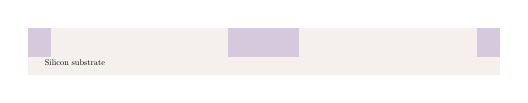
\begin{tikzpicture}[node distance = 3cm, auto, thick,scale=\CrossAndTopSectionBig, every node/.style={transform shape}]
		% substrate
\fill[substrate] (0,0) rectangle (20,2);
\node at (2,0.5) {Silicon substrate};
%trenches
\fill[isolationoxide] (0,0.75) rectangle (1,2);
\fill[isolationoxide] (8.5,0.75) rectangle (11.5,2);
\fill[isolationoxide] (19,0.75) rectangle (20,2);
	\end{tikzpicture}
	
\begin{tikzpicture}[node distance = 3cm, auto, thick,scale=\CrossAndTopSectionBig, every node/.style={transform shape}]
		% substrate
\fill[YellowOrange] (0,0) rectangle (20,12);
% trench area
\fill[DarkGray] (0,0) rectangle (1,12);
\fill[DarkGray] (8.5,0) rectangle (11.5,12);
\fill[DarkGray] (19,0) rectangle (20,12);
\fill[DarkGray] (0,0) rectangle (20,1.25);
\fill[DarkGray] (0,7.5) rectangle (20,12);
	\end{tikzpicture}
	\caption{Shallow trench isolation target geometry}
	\label{sti_target}
\end{figure}

As can be seen in \autoref{nwell_target}, the n-well and the STI trench are supposed to have approximately the same depth but the n-well and p-well go down a little bit further.
Because the n-well will be $\approx 4 \mu m$ in depth we have to match this with our trench depth.
I order to allow a sufficiently low resistance of the ESD diode but at the same time a sufficient isolation of between the standard cells a trade-ff has been done.
The targeted depth of the box isolation is $\approx 2 \mu m$.

\begin{figure}[H]
	\centering
	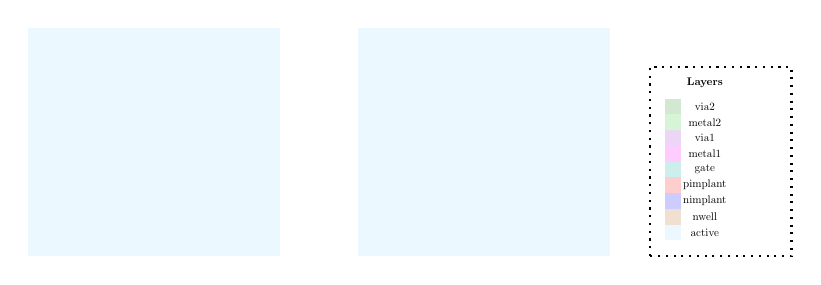
\begin{tikzpicture}[node distance =1cm, auto, thick,scale=\VLSILayout, every node/.style={transform shape}]
		\fill[nwell,opacity=0.2] (0.75,0.5) rectangle (8.75,7.75);
\fill[nwell,opacity=0.2] (11.25,0.5) rectangle (19.25,7.75);

\draw[dotted] (20.5,0.5) rectangle (25,6.5);

\node at (22.25,6) {\textbf{Layers}};

\fill[nwell,opacity=0.2] (21,1) rectangle (21.5,1.5);
\node at (22.25,1.25) {active};

\fill[resist,opacity=0.2] (21,1.5) rectangle (21.5,2);
\node at (22.25,1.75) {nwell};

\fill[blue,opacity=0.2] (21,2) rectangle (21.5,2.5);
\node at (22.25,2.25) {nimplant};

\fill[nitride,opacity=0.2] (21,2.5) rectangle (21.5,3);
\node at (22.25,2.75) {pimplant};

\fill[Emerald,opacity=0.2] (21,3) rectangle (21.5,3.5);
\node at (22.25,3.25) {gate};

\fill[Fuchsia,opacity=0.2] (21,3.5) rectangle (21.5,4);
\node at (22.25,3.75) {metal1};

\fill[DarkOrchid,opacity=0.2] (21,4) rectangle (21.5,4.5);
\node at (22.25,4.25) {via1};

\fill[LimeGreen,opacity=0.2] (21,4.5) rectangle (21.5,5);
\node at (22.25,4.75) {metal2};

\fill[ForestGreen,opacity=0.2] (21,5) rectangle (21.5,5.5);
\node at (22.25,5.25) {via2};

	\end{tikzpicture}
	\caption{Shallow trench isolation layout}
	\label{sti_layout}
\end{figure}

In \autoref{sti_layout} we can see the layout for the STI area.
The STI area will be everywhere, where no active areas are.
The field oxide needs to be grown out of trenches which can't be etched out of the silicon by using resist as a mask.
For that reason we will have to resort to a protective mask made from a silicon dioxide layer which has to be etched before hand.
So the mask will be exposed onto positive resist on top of the hard mask oxide layer in order to form a protective mask covering the active areas from having etched trenches into them.
After that we can either use a dry etching method or wet etching for cutting into the silicon substrate and making the active area become islands with trenches in between.
After these steps we have to remove the hard mask.
Our minimum width and height as well as the space between the active areas comes from the line space constrain of the silicon etcher and of course the optical limitations of the stepper which are as well 0.5\um.

\newpage

\subsection{Initial cleaning}
In order to remove the initial naturally grown silicon dioxide from the wafer, acid is being applied to the wafer which leads to a pure silicon substrate wafer as in the process illustration shown in \autoref{initial_cleaning}.

\begin{figure}[H]
	\centering
	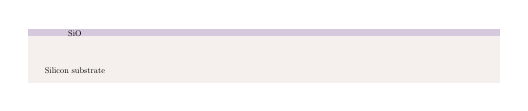
\begin{tikzpicture}[node distance = 3cm, auto, thick,scale=\CrossSectionOnly, every node/.style={transform shape}]
		% substrate
\fill[substrate] (0,0) rectangle (20,2);
\node at (2,0.5) {Silicon substrate};
% oxide
\fill[isolationoxide] (0,2) rectangle (20,2.3);
\node at (2,2.1) {SiO};
	\end{tikzpicture}
	\drawStepArrow{}
	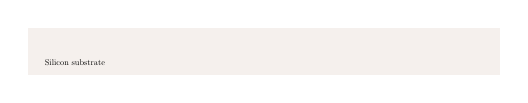
\begin{tikzpicture}[node distance = 3cm, auto, thick,scale=\CrossSectionOnly, every node/.style={transform shape}]
		% substrate
\fill[substrate] (0,0) rectangle (20,2);
\node at (2,0.5) {Silicon substrate};
	\end{tikzpicture}
	\caption{Initial cleaning}
	\label{initial_cleaning}
\end{figure}

This needs to be done because the naturally grown initially existing silicon oxide is not pure and may contain contamination which may render the final product unusable.

\subsubsection{Sulfuric Cleaning}
The sulfuric acid mixture, $H_2 S O_4 + H_2 O_2$ is being applied to the wafer for 10 minutes at a temperature of 120 \degree C.

\subsubsection{HF dip}
After the sulfuric cleaning a HF (HF:$H_2O$,1:50) dip is being performed for one minute. \\
Hydrofluoric acid (HF) is used to remove native silicon dioxide from wafers. Since it acts quickly, one needs to only expose the wafer for a short time ("dip").

\subsubsection{Drying}
After that the wafer needs to be dried and quickly processed further before new uncontrolled natural oxide can build up on the wafer through the contact with air.

\newpage

\subsection{Hard mask: Oxide growth}
We need a thick layer of oxide as protective hard mask to etch the trenches into the silicon.

\begin{figure}[H]
	\centering
	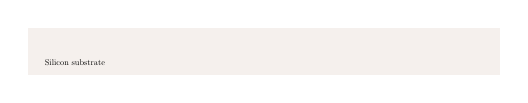
\begin{tikzpicture}[node distance = 3cm, auto, thick,scale=\CrossSectionOnly, every node/.style={transform shape}]
		% substrate
\fill[substrate] (0,0) rectangle (20,2);
\node at (2,0.5) {Silicon substrate};
	\end{tikzpicture}
	\drawStepArrow{Wet oxidation}
	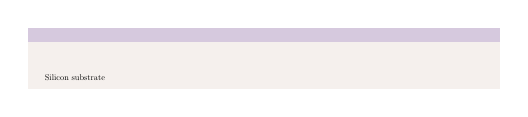
\begin{tikzpicture}[node distance = 3cm, auto, thick,scale=\CrossSectionOnly, every node/.style={transform shape}]
		% substrate
\fill[substrate] (0,0) rectangle (20,2);
\node at (2,0.5) {Silicon substrate};
\fill[isolationoxide] (0,2) rectangle (20,2.6);
	\end{tikzpicture}
	\caption{Hard mask growth}
\end{figure}

In \autoref{sti_trench_etch}.we want to etch 2\um deep into the silicon which, depending on the approach, will take a different amount of oxide for an effective hard mask. \\

\begin{mdframed}[linewidth=2pt,linecolor=red]
For now we only have the plasma etcher variant being verified because chemically etching the silicon wafer with KOH isn't allowed at the HKUST labs for contamination control reasons.
In case you can verify this in your lab with a chemical etching method, please update this chapter and make a pull request!
\end{mdframed}

\textbf{Possible approaches}:
\begin{itemize}
	\item \textbf{"DRIE Etcher \#1" from HKUST} \\
	We can use anisotropic plasma etching for sharper borders. \\
	With this method it takes pretty much a minute to etch 2\um deep. \\
	In one minute the oxide will have been etched away by at most 25nm. \\
	This means we can grow a 100nm thick layer and are well off. \\
	Growing 100nm of dioxide takes around 5 minutes 30 seconds at 1050\degreesC in wet ambient\footnote{\url{http://cleanroom.byu.edu/OxideTimeCalc}}.
	\item \textbf{Chemical solution} \\
	When using KOH acid at 60\degreesC,  it takes 4 minutes and 30 seconds in order to etch 2\um deep. \\
	This means the oxide layer needs to be at least 226 nm thick, so we choose a nice round number of 300nm. \\
	The layer of silicon dioxide of around 300nm thickness is grown in wet ambient for 25 minutes at 1050\degreesC\footnote{\url{http://cleanroom.byu.edu/OxideTimeCalc}} in the diffusion furnace.
\end{itemize}

\subsection{Hard mask: Patterning}

The resist is being deposited using spin coating and then soft baked depending on the baking time for the specific resist.
The requirement is a \textbf{positive} tone resist.

\begin{figure}[H]
	\centering
	\begin{tikzpicture}[node distance = 3cm, auto, thick,scale=\CrossSectionOnly, every node/.style={transform shape}]
		\input{tikz_process_steps/sti.hard_mask_oxide_growth.a.tex}
\fill[isolationoxide] (0,2) rectangle (20,2.6);
	\end{tikzpicture}
	\drawStepArrow{Mask: active}
	\begin{tikzpicture}[node distance = 3cm, auto, thick,scale=\CrossSectionOnly, every node/.style={transform shape}]
		\input{tikz_process_steps/sti.hard_mask_oxide_growth.a.tex}
\fill[isolationoxide] (0,2) rectangle (20,2.6);
\fill[resist] (1,2.6) rectangle (8,3.2);
\fill[resist] (11.5,2.6) rectangle (19,3.2);
	\end{tikzpicture}
	\caption{Patterning with positive resist}
\end{figure}

The layout for being exposed onto the resist is being extracted from the "active" layer within the GDS2 file onto a  onto a \textbf{bright field} mask because we need to use the same mask again in \autoref{fox_chapter}, so alignment needs to be possible.

\newpage

\subsection{Hard mask: Etching}\label{sti_mask_etch}

We open the access to the silicon, outside of the active areas, in order to etch the trenches.

\begin{figure}[H]
	\centering
	\begin{tikzpicture}[node distance = 3cm, auto, thick,scale=\CrossSectionOnly, every node/.style={transform shape}]
		\input{tikz_process_steps/sti.hard_mask_oxide_growth.b.tex}
\fill[resist] (1,2.6) rectangle (8,3.2);
\fill[resist] (11.5,2.6) rectangle (19,3.2);
	\end{tikzpicture}
	\drawStepArrow{}
	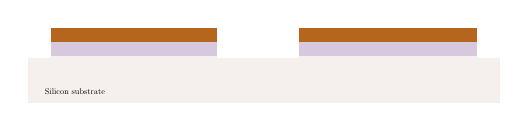
\begin{tikzpicture}[node distance = 3cm, auto, thick,scale=\CrossSectionOnly, every node/.style={transform shape}]
		% substrate
\fill[substrate] (0,0) rectangle (20,1.9);
\node at (2,0.5) {Silicon substrate};

% substrate islands
\fill[substrate] (1,1.9) rectangle (8,2);
\fill[substrate] (11.5,1.9) rectangle (19,2);

% pad oxide
\fill[isolationoxide] (1,2) rectangle (8,2.6);
\fill[isolationoxide] (11.5,2) rectangle (19,2.6);

% resist
\fill[resist] (1,2.6) rectangle (8,3.2);
\fill[resist] (11.5,2.6) rectangle (19,3.2);
	\end{tikzpicture}
	\caption{Nitride mask etching}
\end{figure}

There are dry etching and wet etching methods available for etching the oxide hard mask. The downside of wet etching is that it also etches horizontally, however the chemical BHF is readily available and allows for easy implementation of the process.\\

\textbf{Possible approaches}:
\begin{itemize}
	\item \textbf{"DRIE Etcher \#1" from HKUST} \\
	We can use anisotropic plasma etching for sharper borders.
	\item \textbf{Chemical solution} \\
	We can use buffered hydrofluoric acid (BOE (1:6)) at room temperature for a little bit over 3 minutes in order to get through the 300nm of oxide or around 1 minute for 100nm.in case RIE is being used for silicon etching\\
	Etching too long might cause under-etch however!
\end{itemize}

\subsection{Hard mask: Resist removal}

Now we need to remove the contaminants for further processing.

\begin{figure}[H]
	\centering
	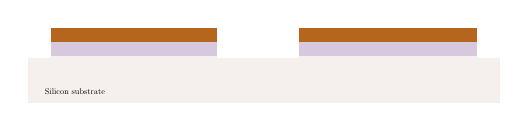
\begin{tikzpicture}[node distance = 3cm, auto, thick,scale=\CrossSectionOnly, every node/.style={transform shape}]
		% substrate
\fill[substrate] (0,0) rectangle (20,1.9);
\node at (2,0.5) {Silicon substrate};

% substrate islands
\fill[substrate] (1,1.9) rectangle (8,2);
\fill[substrate] (11.5,1.9) rectangle (19,2);

% pad oxide
\fill[isolationoxide] (1,2) rectangle (8,2.6);
\fill[isolationoxide] (11.5,2) rectangle (19,2.6);

% resist
\fill[resist] (1,2.6) rectangle (8,3.2);
\fill[resist] (11.5,2.6) rectangle (19,3.2);
	\end{tikzpicture}
	\drawStepArrow{}
	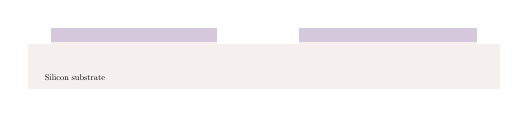
\begin{tikzpicture}[node distance = 3cm, auto, thick,scale=\CrossSectionOnly, every node/.style={transform shape}]
		% substrate
\fill[substrate] (0,0) rectangle (20,1.9);
\node at (2,0.5) {Silicon substrate};

% substrate islands
\fill[substrate] (1,1.9) rectangle (8,2);
\fill[substrate] (11.5,1.9) rectangle (19,2);

% pad oxide
\fill[isolationoxide] (1,2) rectangle (8,2.6);
\fill[isolationoxide] (11.5,2) rectangle (19,2.6);
	\end{tikzpicture}
	\caption{Resist removal}
\end{figure}

We strip the resist, rinse and perform sulfuric cleaning.

\newpage

\subsection{Silicon etching}\label{sti_trench_etch}

Silicon can only be etched by a very aggressive chemical cocktail of  KOH and TMAH (20\%) or by plasma etching.

\begin{figure}[H]
	\centering
	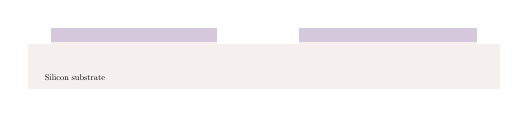
\begin{tikzpicture}[node distance = 3cm, auto, thick,scale=\CrossSectionOnly, every node/.style={transform shape}]
		% substrate
\fill[substrate] (0,0) rectangle (20,1.9);
\node at (2,0.5) {Silicon substrate};

% substrate islands
\fill[substrate] (1,1.9) rectangle (8,2);
\fill[substrate] (11.5,1.9) rectangle (19,2);

% pad oxide
\fill[isolationoxide] (1,2) rectangle (8,2.6);
\fill[isolationoxide] (11.5,2) rectangle (19,2.6);
	\end{tikzpicture}
	\drawStepArrow{}
	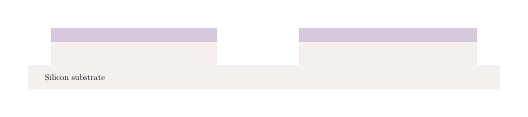
\begin{tikzpicture}[node distance = 3cm, auto, thick,scale=\CrossSectionOnly, every node/.style={transform shape}]
		% substrate
\fill[substrate] (0,0) rectangle (20,1);
\node at (2,0.5) {Silicon substrate};

% substrate islands
\fill[substrate] (1,1) rectangle (8,2);
\fill[substrate] (11.5,1) rectangle (19,2);

% pad oxide
\fill[isolationoxide] (1,2) rectangle (8,2.6);
\fill[isolationoxide] (11.5,2) rectangle (19,2.6);
	\end{tikzpicture}
	\caption{Trench etching}
\end{figure}

\begin{mdframed}[linewidth=2pt,linecolor=red]
For now we only have the plasma etcher variant being verified because chemically etching the silicon wafer with KOH isn't allowed at the HKUST labs for contamination control reasons.
In case you can verify this in your lab with a chemical etching method, please update this chapter and make a pull request!
\end{mdframed}

\textbf{Possible approaches}:
\begin{itemize}
\item \textbf{"DRIE Etcher \#1" from HKUST} \\
This machine a normal etching rate of up to $2\frac{\mu m}{min}$ for etching silicon. \\
This means we etch for 1 minute in order to reach the desired depth. \\
The selectivity to oxide is >80:1 which means the etch speed for the hard mask will be at most $\frac{1}{80}2\frac{\mu m}{min}=\frac{1}{80}2000\frac{nm}{min}=25\frac{nm}{min}$.
\item \textbf{Chemical solution} \\
Using a KOH solution of 20\% at 60\degreesC gives us an etch rate of roughly  26.57\um per hour\footnote{\url{http://www.lelandstanfordjunior.com/KOH.html}}.
\begin{itemize}
\item The <100> etch rate is: 26.57 micron/hr = 0.44 micron/min
\item The <110> etch rate is: 40.5 micron/hr 
\item The <111> etch rate is: 0.4932 micron/hr 
\item The SiO2 etch rate is: 49.92 nanometers/hr 
\end{itemize}
With a desired depth of 2\um we will have to etch around 4 minutes and 30 seconds in order to reach the desired depth.
The disadvantage of this approach is the imprecision and under-etch of the mask.
\end{itemize}

\subsection{Hard mask: Removal}

Now we have to remove the oxide hard mask for further processing in order to proceed with well formation without contamination during oxide growing.

\begin{figure}[H]
	\centering
	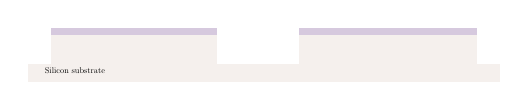
\begin{tikzpicture}[node distance = 3cm, auto, thick,scale=\CrossSectionOnly, every node/.style={transform shape}]
		% substrate
\fill[substrate] (0,0) rectangle (20,0.75);
\node at (2,0.5) {Silicon substrate};

% substrate islands
\fill[substrate] (1,0.75) rectangle (8,2);
\fill[substrate] (11.5,0.75) rectangle (19,2);

% covering oxide
\fill[isolationoxide] (1,2) rectangle (8,2.3);
\fill[isolationoxide] (11.5,2) rectangle (19,2.3);
	\end{tikzpicture}
	\drawStepArrow{}
	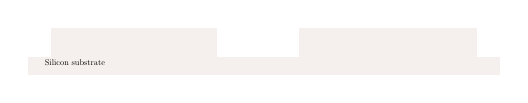
\begin{tikzpicture}[node distance = 3cm, auto, thick,scale=\CrossSectionOnly, every node/.style={transform shape}]
		% substrate
\fill[substrate] (0,0) rectangle (20,0.75);
\node at (2,0.5) {Silicon substrate};

% substrate islands
\fill[substrate] (1,0.75) rectangle (8,2);
\fill[substrate] (11.5,0.75) rectangle (19,2);
	\end{tikzpicture}
	\caption{Trench etching}
\end{figure}

We use buffered hydrofluoric acid (BOE (1:6)) at room temperature for a little bit over 3 minutes in order to remove all of the 300nm thick oxide layer and roughly 1 minute for 100nm.


\newpage
`\section{P-well}\label{pwell_chapter}
In order to build CMOS on the same substrate, a P-well is required for building the complementary N-channel transistor for a n-p-channel logic circuitry.
The cross section as well as the top view of the targeted geometry are shown in \autoref{nwell_target}
\begin{figure}[H]
	\centering
	\begin{tikzpicture}[node distance = 3cm, auto, thick,scale=\CrossAndTopSectionBig, every node/.style={transform shape}]
		\input{tikz_process_steps/sti.a.tex}
% n-well
\fill[nwell] (1.25,0.75) rectangle (8.5,2);
\node at (5.75,1) {N-Well};


% p-well
\fill[pwell] (11.75,0.75) rectangle (18.75,2);
\node at (14.25,1) {P-Well};
	\end{tikzpicture}
	\begin{tikzpicture}[node distance = 3cm, auto, thick,scale=\CrossAndTopSectionBig, every node/.style={transform shape}]
		\input{tikz_process_steps/sti.b.tex}
\fill[nwell] (1.25,1) rectangle (8.25,7.25);
\fill[pwell] (11.75,1) rectangle (18.75,7.25);
	\end{tikzpicture}
	\caption{P-well target geometry}
	\label{pwell_target}
\end{figure}
The P-well will serve us as an island of higher p-doped substrate within the slightly p-doped basis substrate.

The dopant dose will be $2.5\times10^{12}cm^{-2}$ as calculated in the documentation of the process design leading to these steps\footnote{\url{https://github.com/leviathanch/libresiliconprocess/raw/master/process_design/process_design.pdf}}.

\begin{figure}[H]
	\centering
	\begin{tikzpicture}[node distance =1cm, auto, thick,scale=\VLSILayout, every node/.style={transform shape}]
		\input{tikz_process_steps/sti.layout.tex}
\fill[nwell,opacity=\OpacityLayout] (1,0.75) rectangle (8.5,7.5);
\fill[pwell,opacity=\OpacityLayout] (11.5,0.75) rectangle (19,7.5);
	\end{tikzpicture}
	\caption{P-Well layout}
	\label{pwell_layout}
\end{figure}

In \autoref{pwell_layout} the layout of the P-well region on top of the active area region can be seen.

The p-well is being fit into the active area.

It should even be a little bit bigger than the active area, because of possible alignment offsets

\newpage

\subsection{Hard mask: Dioxide growth}

In order to selectively inject charge carrying atoms into the crystalline structure a protective dioxide ($SiO_2$) layer needs to be grown on top of a p-type substrate.

\begin{figure}[H]
	\centering
	\begin{tikzpicture}[node distance = 3cm, auto, thick,scale=\CrossSectionOnly, every node/.style={transform shape}]
		\input{tikz_process_steps/sti.a.tex}
% n-well
\fill[nwell] (1.25,0.75) rectangle (8.5,2);
\node at (5.75,1) {N-Well};


	\end{tikzpicture}
	\drawStepArrow{Wet oxidation}
	\begin{tikzpicture}[node distance = 3cm, auto, thick,scale=\CrossSectionOnly, every node/.style={transform shape}]
		% oxide
\fill[isolationoxide] (0,1.25) rectangle (20,2.75);

% oxide hill 1
\fill[isolationoxide] (1.25,2.75) rectangle (8.25,3.5);
\filldraw[line width=0, isolationoxide] (0.5,2.75) -- (1.25,2.75) -- (1.25,3.5);
\filldraw[line width=0, isolationoxide] (8.25,2.75) -- (8.25,3.5) -- (9.0,2.75);

% oxide hill 2
\fill[isolationoxide] (11.75,2.75) rectangle (18.75,3.5);
\filldraw[line width=0, isolationoxide] (11.0,2.75) -- (11.75,2.75) -- (11.75,3.5);
\filldraw[line width=0, isolationoxide] (18.75,2.75) -- (18.75,3.5) -- (19.5,2.75);

\node at (2,2.1) {SiO2};

\input{tikz_process_steps/nwell.a.tex}
	\end{tikzpicture}
	\caption{Dioxide layer growth}
\end{figure}

With an energy of 100keV for the implantation performed in \autoref{pwell_implant_step}, the projected range of the dopants within the oxide will be 310nm (380nm tops) \footnote{\url{http://cleanroom.byu.edu/rangestraggle}}.
This means being on the safe side and having 500nm as the thickness is a good approach.

In order to grow the 500nm thick oxide layer, the wafer is being oxidized for around 56 minutes at 1050\degree C using wet oxidation which results in a dioxide layer of around 500nm in thickness\footnote{\url{http://cleanroom.byu.edu/OxideTimeCalc}}.

\subsection{Hard mask: Patterning}

The resist is being deposited spray or spin coating (spray coating is better because of the uneven surface!) and then soft baked depending on the baking time for the specific resist.
The layout for being exposed onto the resist is being extracted from the "pwell" layer within the GDS2 file onto a \textbf{bright field} mask.
The requirement is a \textbf{negative} tone resist.

\begin{figure}[H]
	\centering
	\begin{tikzpicture}[node distance = 3cm, auto, thick,scale=\CrossAndTopSection, every node/.style={transform shape}]
		% oxide
\fill[isolationoxide] (0,1.25) rectangle (20,2.75);

% oxide hill 1
\fill[isolationoxide] (1.25,2.75) rectangle (8.25,3.5);
\filldraw[line width=0, isolationoxide] (0.5,2.75) -- (1.25,2.75) -- (1.25,3.5);
\filldraw[line width=0, isolationoxide] (8.25,2.75) -- (8.25,3.5) -- (9.0,2.75);

% oxide hill 2
\fill[isolationoxide] (11.75,2.75) rectangle (18.75,3.5);
\filldraw[line width=0, isolationoxide] (11.0,2.75) -- (11.75,2.75) -- (11.75,3.5);
\filldraw[line width=0, isolationoxide] (18.75,2.75) -- (18.75,3.5) -- (19.5,2.75);

\node at (2,2.1) {SiO2};

\input{tikz_process_steps/pwell.mask_dioxide_layer.a.tex}
	\end{tikzpicture}
	
\begin{tikzpicture}[node distance = 3cm, auto, thick,scale=\CrossAndTopSection, every node/.style={transform shape}]
		% resist
\fill[isolationoxide] (0,0) rectangle (20,12);
	\end{tikzpicture}
	\drawStepArrow{Mask: pwell}
	\begin{tikzpicture}[node distance = 3cm, auto, thick,scale=\CrossAndTopSection, every node/.style={transform shape}]
		% resist
\fill[resist] (0.25,2.0) rectangle (11.5,5.0);
\fill[resist] (19,2.0) rectangle (19.75,5.0);

\input{tikz_process_steps/pwell.mask_dioxide_layer.b.tex}

	\end{tikzpicture}
	
\begin{tikzpicture}[node distance = 3cm, auto, thick,scale=\CrossAndTopSection, every node/.style={transform shape}]
		% resist
\fill[resist] (0,0) rectangle (20,12);
% substrate
\fill[isolationoxide] (11.5,1.5) rectangle (19,7.25);
	\end{tikzpicture}
	\caption{Cross/top view of P-well layout on resist}
\end{figure}
The thickness of the resist layer and the baking duration will variate depending on the specific equipment for which this process will be implemented with.
Also after the exposure and development, the hard baking shouldn't be forgotten!

\newpage

\subsection{Hard mask: Etching}
We now need to open a window in the dioxide layer, through which we will inject carrier atoms into the silicon crystal structure.
\begin{figure}[H]
	\centering
	\begin{tikzpicture}[node distance = 3cm, auto, thick,scale=\CrossAndTopSection, every node/.style={transform shape}]
		% resist
\fill[resist] (0.25,2.0) rectangle (11.5,5.0);
\fill[resist] (19,2.0) rectangle (19.75,5.0);

\input{tikz_process_steps/pwell.patterning.a.tex}

	\end{tikzpicture}
	
\begin{tikzpicture}[node distance = 3cm, auto, thick,scale=\CrossAndTopSection, every node/.style={transform shape}]
		% resist
\fill[resist] (0,0) rectangle (20,12);
% substrate
\fill[isolationoxide] (1.25,1.5) rectangle (8.25,7.25);
	\end{tikzpicture}
	\drawStepArrow{}
	\begin{tikzpicture}[node distance = 3cm, auto, thick,scale=\CrossAndTopSection, every node/.style={transform shape}]
		% resist
\fill[resist] (0,2.6) rectangle (11.5,5.0);
\fill[resist] (19,2.6) rectangle (20,5.0);

% oxide
\fill[isolationoxide] (0,1.25) rectangle (11.5,2.75);
\fill[isolationoxide] (19,1.25) rectangle (20,2.75);

% oxide hill 1
\fill[isolationoxide] (1.25,2.75) rectangle (8.25,3.5);
\filldraw[line width=0, isolationoxide] (0.5,2.75) -- (1.25,2.75) -- (1.25,3.5);
\filldraw[line width=0, isolationoxide] (8.25,2.75) -- (8.25,3.5) -- (9.0,2.75);

% oxide hill 2
\filldraw[line width=0, isolationoxide] (11.25,2.75) -- (11.5,2.75) -- (11.5,3.0);
\filldraw[line width=0, isolationoxide] (19.0,3.0)  -- (19.0,2.75) -- (19.00,2.75);

\node at (2,2.1) {SiO2};

\input{tikz_process_steps/nwell.a.tex}


	\end{tikzpicture}
	
\begin{tikzpicture}[node distance = 3cm, auto, thick,scale=\CrossAndTopSection, every node/.style={transform shape}]
		% resist
\fill[resist] (0,0) rectangle (20,12);
% substrate
\fill[substrate] (1.25,1.5) rectangle (8.25,7.25);
	\end{tikzpicture}
	\caption{Cross/top view of P-well oxide window}
\end{figure}

There are multiple possible approaches to etch through these 500nm of oxide.\\

\textbf{Possible approaches}:
\begin{itemize}
	\item \textbf{"AOE Etcher (DRY-AOE)" from HKUST} \\
	We can use anisotropic plasma etching for sharper borders.
	\item \textbf{Chemical solution} \\
	We can use buffered hydrofluoric acid (BOE (1:6)) at room temperature for 5 minutes in order to get through the 500nm of oxide.\\
	Too long over 4 minutes might cause under-etch however!
\end{itemize}

\subsection{Hard mask: Resist strip}

In order to avoid contamination of the machines we need to make sure all the resist has been stripped off from the wafer.

\begin{figure}[H]
	\centering
	\begin{tikzpicture}[node distance = 3cm, auto, thick,scale=\CrossSectionOnly, every node/.style={transform shape}]
		\input{tikz_process_steps/pwell.patterning.b.tex}

% boron
\shade[upper left = pwell, upper right = pwell, lower right = substrate, lower left = substrate,] (11.5,1.5) rectangle (19.0,2);


	\end{tikzpicture}
	\drawStepArrow{}
	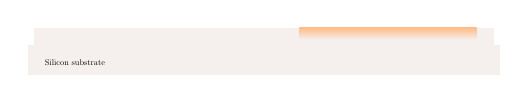
\begin{tikzpicture}[node distance = 3cm, auto, thick,scale=\CrossSectionOnly, every node/.style={transform shape}]
		% substrate
\fill[substrate] (0,0) rectangle (20,1.25);
\node at (2,0.5) {Silicon substrate};
\fill[substrate] (0.25,1.25) rectangle (19.75,2);

% boron
\shade[upper left = pwell, upper right = pwell, lower right = substrate, lower left = substrate,] (11.5,1.5) rectangle (19.0,2);

	\end{tikzpicture}
	\caption{Resist removal}
\end{figure}
Please just use the solvent for the specific resist.

\newpage

\subsection{Implantation/Doping}\label{pwell_implant_step}
We now need to inject the carriers into the upper level of the n-channel area so that we can later on drive them into the crystal during the drive-in step.

\begin{figure}[H]
	\centering
	\begin{minipage}{0.5\textwidth}
	\centering
	\begin{tikzpicture}[node distance = 3cm, auto, thick,scale=\CrossSectionOnly, every node/.style={transform shape}]
		% oxide
\fill[isolationoxide] (0,1.25) rectangle (11.5,2.75);
\fill[isolationoxide] (19,1.25) rectangle (20,2.75);

% oxide hill 1
\fill[isolationoxide] (1.25,2.75) rectangle (8.25,3.5);
\filldraw[line width=0, isolationoxide] (0.5,2.75) -- (1.25,2.75) -- (1.25,3.5);
\filldraw[line width=0, isolationoxide] (8.25,2.75) -- (8.25,3.5) -- (9.0,2.75);

% oxide hill 2
\filldraw[line width=0, isolationoxide] (11.25,2.75) -- (11.5,2.75) -- (11.5,3.0);
\filldraw[line width=0, isolationoxide] (19.0,3.0)  -- (19.0,2.75) -- (19.25,2.75);

\node at (2,2.1) {SiO2};

\input{tikz_process_steps/nwell.a.tex}

\forloop{ct}{0}{\value{ct} < 21}
{
	\draw [->] (\value{ct},5) -- (\value{ct},4);
	\node at (\value{ct},5.2) {P$^{31}$};
}
	\end{tikzpicture}
	\drawStepArrow{Boron implant}
	\begin{tikzpicture}[node distance = 3cm, auto, thick,scale=\CrossSectionOnly, every node/.style={transform shape}]
		% resist
\fill[resist] (0.25,2.0) rectangle (11.5,5.0);
\fill[resist] (19,2.0) rectangle (19.75,5.0);

\input{tikz_process_steps/pwell.patterning.a.tex}


% boron
\shade[upper left = pwell, upper right = pwell, lower right = substrate, lower left = substrate,] (11.5,1.5) rectangle (19.0,2);

	\end{tikzpicture}
	\drawStepArrow{Annealing}
	\begin{tikzpicture}[node distance = 3cm, auto, thick,scale=\CrossSectionOnly, every node/.style={transform shape}]
		% oxide
\fill[isolationoxide] (0,1.25) rectangle (11.5,2.75);
\fill[isolationoxide] (19,1.25) rectangle (20,2.75);

% oxide hill 1
\fill[isolationoxide] (1.25,2.75) rectangle (8.25,3.5);
\filldraw[line width=0, isolationoxide] (0.5,2.75) -- (1.25,2.75) -- (1.25,3.5);
\filldraw[line width=0, isolationoxide] (8.25,2.75) -- (8.25,3.5) -- (9.0,2.75);

% oxide hill 2
\filldraw[line width=0, isolationoxide] (11.25,2.75) -- (11.5,2.75) -- (11.5,3.0);
\filldraw[line width=0, isolationoxide] (19.0,3.0)  -- (19.0,2.75) -- (19.25,2.75);

\node at (2,2.1) {SiO2};

\input{tikz_process_steps/nwell.a.tex}

% boron
\fill[pwell] (11.75,1.5) rectangle (18.75,2);
	\end{tikzpicture} \\
	\textbf{Implantation approach}
	\end{minipage}\begin{minipage}{0.5\textwidth}
	\centering
	\begin{tikzpicture}[node distance = 3cm, auto, thick,scale=\CrossSectionOnly, every node/.style={transform shape}]
		% boron
\fill[pwell] (0,0) rectangle (20,5);

\input{tikz_process_steps/basic.a.tex}
% boron
\shade[upper left = pwell, upper right = pwell, lower right = substrate, lower left = substrate,] (11.5,1.5) rectangle (19.0,2);

	\end{tikzpicture}
	\drawStepArrow{Constant source diffusion}
	\begin{tikzpicture}[node distance = 3cm, auto, thick,scale=\CrossSectionOnly, every node/.style={transform shape}]
		% boron
\fill[pwell] (0,0) rectangle (20,5);

\input{tikz_process_steps/basic.a.tex}
% boron
\shade[upper left = pwell, upper right = pwell, lower right = substrate, lower left = substrate,] (11.5,1.5) rectangle (19.0,2);


% boron
\shade[upper left = pwell, upper right = pwell, lower right = substrate, lower left = substrate,] (11.75,1.5) rectangle (18.75,2);
	\end{tikzpicture}
	\drawStepArrow{Source removal}
	\begin{tikzpicture}[node distance = 3cm, auto, thick,scale=\CrossSectionOnly, every node/.style={transform shape}]
		\input{tikz_process_steps/basic.a.tex}
% boron
\shade[upper left = pwell, upper right = pwell, lower right = substrate, lower left = substrate,] (11.5,1.5) rectangle (19.0,2);


% boron
\shade[upper left = pwell, upper right = pwell, lower right = substrate, lower left = substrate,] (11.75,1.5) rectangle (18.75,2);
	\end{tikzpicture} \\
	\textbf{Diffusion approach}
	\end{minipage}
	\caption{Doping process}
\end{figure}

\textbf{Possible approaches}:
\begin{itemize}
	\item \textbf{"CF-3000 Implanter (IMP-3000)" from HKUST} \\
	At HKUST we have an implanter which gives us better control over the initial surface concentration. \\
	These steps are needed to arrive with the desired geometry:
	\begin{enumerate}
		\item The P-well is implanted with a Boron ($B^{11}$) dose of $2.5\times10^{12}cm^{-2}$ at an energy of 100 keV
		\item The P-well is annealed for 30 minutes at 1050\degreesC in $N_2$ environment (DIF-A1)\\
		After that the P-well will be around 1\um deep and will become deeper during \autoref{nwell_implant_step}
	\end{enumerate}
	\item \textbf{Constant source diffusion} \\
	We can add a layer of Boron solution and diffusing in order to have an initial concentration in order to reach the desired concentration later by main diffusion.
	\begin{enumerate}
		\item A constant source is added (gas or liquid)
		\item The source dopant is driven in for 10 minutes at 1050\degreesC
		\item The dopant source is removed by stopping the gas flow or cleaning the surface
	\end{enumerate}
\end{itemize}

\subsection{Hard mask: Removal}

Now we want to remove the silicon mask from the wafer and clean it for another clean oxide mask layer in order to perform the implantation of the N-well in the next step.

\begin{figure}[H]
	\centering
	\begin{tikzpicture}[node distance = 3cm, auto, thick,scale=\CrossSectionOnly, every node/.style={transform shape}]
		\input{tikz_process_steps/nwell.a.tex}

% boron
\fill[pwell] (11.5,1.8) rectangle (19,2);
\fill[pwell] (0,2.5) rectangle (11.5,2.6);
\fill[pwell] (19,2.5) rectangle (20,2.6);

% oxide
\fill[isolationoxide] (0,2) rectangle (11.5,2.6);
\fill[isolationoxide] (19,2) rectangle (20,2.6);
\fill[isolationoxide] (1.5,2) rectangle (19,2.3); % cover

% pwell
\fill[pwell] (11.75,0.75) rectangle (18.75,2);
	\end{tikzpicture}
	\drawStepArrow{}
	\begin{tikzpicture}[node distance = 3cm, auto, thick,scale=\CrossSectionOnly, every node/.style={transform shape}]
		\input{tikz_process_steps/nwell.a.tex}

% pwell
\fill[pwell] (11.75,0.75) rectangle (18.75,2);
\node at (14.25,1) {P-Well};
	\end{tikzpicture}
	\caption{Oxide removal}
\end{figure}

We use buffered hydrofluoric acid (BOE (1:6)) at room temperature for 5 minutes in order to remove the 500nm of oxide layer.
\newpage
\section{N-well}\label{nwell_chapter}
In order to build CMOS on the same substrate, an N-well is required for building the complementary P-channel transistor for a n-p-channel logic circuitry as shown above in the example section.
The cross section as well as the top view of the targeted geometry are shown in \autoref{nwell_target}
\begin{figure}[H]
	\centering
	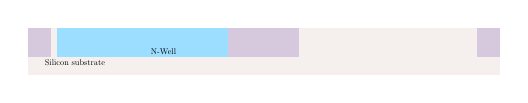
\begin{tikzpicture}[node distance = 3cm, auto, thick,scale=\CrossAndTopSectionBig, every node/.style={transform shape}]
		% substrate
\fill[substrate] (0,0) rectangle (20,2);
\node at (2,0.5) {Silicon substrate};
%trenches
\fill[isolationoxide] (0,0.75) rectangle (1,2);
\fill[isolationoxide] (8.5,0.75) rectangle (11.5,2);
\fill[isolationoxide] (19,0.75) rectangle (20,2);
% n-well
\fill[nwell] (1.25,0.75) rectangle (8.5,2);
\node at (5.75,1) {N-Well};


	\end{tikzpicture}
	
\begin{tikzpicture}[node distance = 3cm, auto, thick,scale=\CrossAndTopSectionBig, every node/.style={transform shape}]
		% substrate
\fill[YellowOrange] (0,0) rectangle (20,12);
% trench area
\fill[DarkGray] (0,0) rectangle (1,12);
\fill[DarkGray] (8.5,0) rectangle (11.5,12);
\fill[DarkGray] (19,0) rectangle (20,12);
\fill[DarkGray] (0,0) rectangle (20,1.25);
\fill[DarkGray] (0,7.5) rectangle (20,12);
\fill[nwell] (1.25,1) rectangle (8.25,7.25);
	\end{tikzpicture}
	\caption{N-well target geometry}
	\label{nwell_target}
\end{figure}

The N-well will serve us as an island of N-doped substrate within the P-doped basis substrate.

The dopant dose will be $2.5\times10^{12}cm^{-2}$ as calculated in the documentation of the process design leading to these steps\footnote{\url{https://github.com/leviathanch/libresiliconprocess/raw/master/process_design/process_design.pdf}}.

\begin{figure}[H]
	\centering
	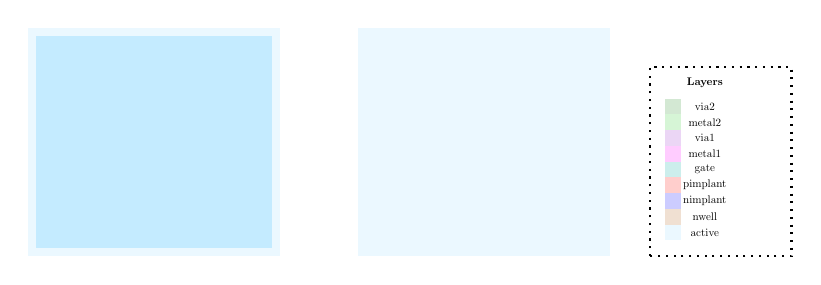
\begin{tikzpicture}[node distance =1cm, auto, thick,scale=\VLSILayout, every node/.style={transform shape}]
		\fill[nwell,opacity=0.2] (0.75,0.5) rectangle (8.75,7.75);
\fill[nwell,opacity=0.2] (11.25,0.5) rectangle (19.25,7.75);

\draw[dotted] (20.5,0.5) rectangle (25,6.5);

\node at (22.25,6) {\textbf{Layers}};

\fill[nwell,opacity=0.2] (21,1) rectangle (21.5,1.5);
\node at (22.25,1.25) {active};

\fill[resist,opacity=0.2] (21,1.5) rectangle (21.5,2);
\node at (22.25,1.75) {nwell};

\fill[blue,opacity=0.2] (21,2) rectangle (21.5,2.5);
\node at (22.25,2.25) {nimplant};

\fill[nitride,opacity=0.2] (21,2.5) rectangle (21.5,3);
\node at (22.25,2.75) {pimplant};

\fill[Emerald,opacity=0.2] (21,3) rectangle (21.5,3.5);
\node at (22.25,3.25) {gate};

\fill[Fuchsia,opacity=0.2] (21,3.5) rectangle (21.5,4);
\node at (22.25,3.75) {metal1};

\fill[DarkOrchid,opacity=0.2] (21,4) rectangle (21.5,4.5);
\node at (22.25,4.25) {via1};

\fill[LimeGreen,opacity=0.2] (21,4.5) rectangle (21.5,5);
\node at (22.25,4.75) {metal2};

\fill[ForestGreen,opacity=0.2] (21,5) rectangle (21.5,5.5);
\node at (22.25,5.25) {via2};

\fill[nwell,opacity=\OpacityLayout] (1,0.75) rectangle (8.5,7.5);
	\end{tikzpicture}
	\caption{N-Well layout}
	\label{nwell_layout}
\end{figure}

In \autoref{nwell_layout} the layout of the n-well region on top of the active area region can be seen.

The n-well is being fit into the active area. It should even be a little bit bigger than the active area, because of possible alignment offsets

\newpage

\subsection{Hard mask: Dioxide growth}

In order to selectively inject charge carrying atoms into the crystalline structure a protective dioxide ($SiO_2$) layer needs to be grown on top of a p-type substrate.

\begin{figure}[H]
	\centering
	\begin{tikzpicture}[node distance = 3cm, auto, thick,scale=\CrossSectionOnly, every node/.style={transform shape}]
		\input{tikz_process_steps/pwell.mask_dioxide_layer.a.tex}

% pwell
\fill[pwell] (11.75,0.75) rectangle (18.75,2);
\node at (14.25,1) {P-Well};
	\end{tikzpicture}
	\drawStepArrow{Wet oxidation}
	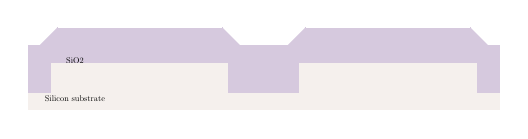
\begin{tikzpicture}[node distance = 3cm, auto, thick,scale=\CrossSectionOnly, every node/.style={transform shape}]
		% oxide
\fill[isolationoxide] (0,1.25) rectangle (20,2.75);

% oxide hill 1
\fill[isolationoxide] (1.25,2.75) rectangle (8.25,3.5);
\filldraw[line width=0, isolationoxide] (0.5,2.75) -- (1.25,2.75) -- (1.25,3.5);
\filldraw[line width=0, isolationoxide] (8.25,2.75) -- (8.25,3.5) -- (9.0,2.75);

% oxide hill 2
\fill[isolationoxide] (11.75,2.75) rectangle (18.75,3.5);
\filldraw[line width=0, isolationoxide] (11.0,2.75) -- (11.75,2.75) -- (11.75,3.5);
\filldraw[line width=0, isolationoxide] (18.75,2.75) -- (18.75,3.5) -- (19.5,2.75);

\node at (2,2.1) {SiO2};

% substrate
\fill[substrate] (0,0) rectangle (20,2);
\node at (2,0.5) {Silicon substrate};
%trenches
\fill[isolationoxide] (0,0.75) rectangle (1,2);
\fill[isolationoxide] (8.5,0.75) rectangle (11.5,2);
\fill[isolationoxide] (19,0.75) rectangle (20,2);
	\end{tikzpicture}
	\caption{Dioxide layer growth}
\end{figure}

With an energy of 100keV for the implantation performed in \autoref{nwell_implant_step}, the projected range of the dopants within the oxide will be 100nm (130nm tops) \footnote{\url{http://cleanroom.byu.edu/rangestraggle}}.
This means being on the safe side and having 200nm as the thickness is a good approach.

In order to grow the 200nm thick oxide layer, the wafer is being oxidized for around 14 minutes at 1050\degree C using wet oxidation which results in a dioxide layer of around 200nm in thickness\footnote{\url{http://cleanroom.byu.edu/OxideTimeCalc}}.

\subsection{Hard mask: Patterning}

The resist is being deposited using spray coating because the uneven nature of the oxide layer.
After that the wafer is being soft baked depending on the baking time and temperature for the specific resist.
The layout for being exposed onto the resist is being extracted from the "nwell" layer within the GDS2 file onto a \textbf{bright field} mask.
The requirement is a \textbf{negative} tone resist.

\begin{figure}[H]
	\centering
	\begin{tikzpicture}[node distance = 3cm, auto, thick,scale=\CrossAndTopSection, every node/.style={transform shape}]
		% oxide
\fill[isolationoxide] (0,1.25) rectangle (20,2.75);

% oxide hill 1
\fill[isolationoxide] (1.25,2.75) rectangle (8.25,3.5);
\filldraw[line width=0, isolationoxide] (0.5,2.75) -- (1.25,2.75) -- (1.25,3.5);
\filldraw[line width=0, isolationoxide] (8.25,2.75) -- (8.25,3.5) -- (9.0,2.75);

% oxide hill 2
\fill[isolationoxide] (11.75,2.75) rectangle (18.75,3.5);
\filldraw[line width=0, isolationoxide] (11.0,2.75) -- (11.75,2.75) -- (11.75,3.5);
\filldraw[line width=0, isolationoxide] (18.75,2.75) -- (18.75,3.5) -- (19.5,2.75);

\node at (2,2.1) {SiO2};

\input{tikz_process_steps/sti.a.tex}
	\end{tikzpicture}
	
\begin{tikzpicture}[node distance = 3cm, auto, thick,scale=\CrossAndTopSection, every node/.style={transform shape}]
		% resist
\fill[isolationoxide] (0,0) rectangle (20,12);
	\end{tikzpicture}
	\drawStepArrow{Mask: nwell}
	\begin{tikzpicture}[node distance = 3cm, auto, thick,scale=\CrossAndTopSection, every node/.style={transform shape}]
		% resist
\fill[resist] (0,2.6) rectangle (1,5.0);
\fill[resist] (8.5,2.6) rectangle (20,5.0);

% oxide
\fill[isolationoxide] (0,1.25) rectangle (20,2.75);

% oxide hill 1
\fill[isolationoxide] (1.25,2.75) rectangle (8.25,3.5);
\filldraw[line width=0, isolationoxide] (0.5,2.75) -- (1.25,2.75) -- (1.25,3.5);
\filldraw[line width=0, isolationoxide] (8.25,2.75) -- (8.25,3.5) -- (9.0,2.75);

% oxide hill 2
\fill[isolationoxide] (11.75,2.75) rectangle (18.75,3.5);
\filldraw[line width=0, isolationoxide] (11.0,2.75) -- (11.75,2.75) -- (11.75,3.5);
\filldraw[line width=0, isolationoxide] (18.75,2.75) -- (18.75,3.5) -- (19.5,2.75);

\node at (2,2.1) {SiO2};

\input{tikz_process_steps/sti.a.tex}
	\end{tikzpicture}
	\begin{tikzpicture}[node distance = 3cm, auto, thick,scale=\CrossAndTopSection, every node/.style={transform shape}]
		% resist
\fill[resist] (0,0) rectangle (20,12);
% substrate
\fill[isolationoxide] (1.25,1.5) rectangle (8.25,7.25);
	\end{tikzpicture}
	\caption{Cross/top view of n-well layout on resist}
\end{figure}

The thickness of the resist layer and the baking duration will variate depending on the specific equipment for which this process will be implemented with.
Also after the exposure and development, the hard baking shouldn't be forgotten!

\newpage

\subsection{Hard mask: Etching}

We now need to open a window in the dioxide layer, through which we will inject carrier atoms into the silicon crystal structure.

\begin{figure}[H]
	\centering
	\begin{tikzpicture}[node distance = 3cm, auto, thick,scale=\CrossAndTopSection, every node/.style={transform shape}]
		% resist
\fill[resist] (0,2.6) rectangle (1,5.0);
\fill[resist] (8.5,2.6) rectangle (20,5.0);

\input{tikz_process_steps/nwell.mask_dioxide_layer.b.tex}
	\end{tikzpicture}
	\begin{tikzpicture}[node distance = 3cm, auto, thick,scale=\CrossAndTopSection, every node/.style={transform shape}]
		% resist
\fill[resist] (0,0) rectangle (20,12);
% substrate
\fill[isolationoxide]  (1,0.75) rectangle (8.5,7.5);
	\end{tikzpicture}
	\drawStepArrow{}
	\begin{tikzpicture}[node distance = 3cm, auto, thick,scale=\CrossAndTopSection, every node/.style={transform shape}]
		% resist
\fill[resist] (0,2.6) rectangle (1,5.0);
\fill[resist] (8.5,2.6) rectangle (20,5.0);

% oxide
\fill[isolationoxide] (0,1.25) rectangle (1,2.75);
\fill[isolationoxide] (8.5,1.25) rectangle (20,2.75);

% oxide hill 1
\filldraw[line width=0, isolationoxide] (0.5,2.75) -- (1.0,2.75) -- (1.0,3.0);
\filldraw[line width=0, isolationoxide] (8.75,2.75) -- (8.5,2.75) -- (8.5,3.0);

% oxide hill 2
\fill[isolationoxide] (11.75,2.75) rectangle (18.75,3.5);
\filldraw[line width=0, isolationoxide] (11.0,2.75) -- (11.75,2.75) -- (11.75,3.5);
\filldraw[line width=0, isolationoxide] (18.75,2.75) -- (18.75,3.5) -- (19.5,2.75);

% substrate
\fill[substrate] (0,0) rectangle (20,2);
\node at (2,0.5) {Silicon substrate};
%trenches
\fill[isolationoxide] (0,0.75) rectangle (1,2);
\fill[isolationoxide] (8.5,0.75) rectangle (11.5,2);
\fill[isolationoxide] (19,0.75) rectangle (20,2);
	\end{tikzpicture}
	\begin{tikzpicture}[node distance = 3cm, auto, thick,scale=\CrossAndTopSection, every node/.style={transform shape}]
		% resist
\fill[resist] (0,0) rectangle (20,12);
% substrate
\fill[substrate] (1.25,1) rectangle (8.25,7.25);
	\end{tikzpicture}
	\caption{Cross/top view of n-well oxide window}
\end{figure}

Since the silicon dioxide layer is 300nm thick and we wanna reach the silicon below we can use wet etching as described in the chemistry chapter.\\

\textbf{Possible approaches}:
\begin{itemize}
	\item \textbf{"AOE Etcher (DRY-AOE)" from HKUST} \\
	We can use anisotropic plasma etching for sharper borders.
	\item \textbf{Chemical solution} \\
	We can use buffered hydrofluoric acid (BOE (1:6)) at room temperature for a little bit over 3 minutes in order to get through the 300nm of oxide.\\
	Too long over 3 minutes might cause under-etch however!
\end{itemize}

\subsection{Hard mask: Resist strip}
In order to avoid contamination of the machines we need to make sure all the resist has been stripped off from the wafer.
\begin{figure}[H]
	\centering
	\begin{tikzpicture}[node distance = 3cm, auto, thick,scale=\CrossSectionOnly, every node/.style={transform shape}]
		% resist
\fill[resist] (0,2.6) rectangle (1,5.0);
\fill[resist] (8.5,2.6) rectangle (20,5.0);

% oxide
\fill[isolationoxide] (0,1.25) rectangle (1,2.75);
\fill[isolationoxide] (8.5,1.25) rectangle (20,2.75);

% oxide hill 1
\filldraw[line width=0, isolationoxide] (0.5,2.75) -- (1.0,2.75) -- (1.0,3.0);
\filldraw[line width=0, isolationoxide] (8.75,2.75) -- (8.5,2.75) -- (8.5,3.0);

% oxide hill 2
\fill[isolationoxide] (11.75,2.75) rectangle (18.75,3.5);
\filldraw[line width=0, isolationoxide] (11.0,2.75) -- (11.75,2.75) -- (11.75,3.5);
\filldraw[line width=0, isolationoxide] (18.75,2.75) -- (18.75,3.5) -- (19.5,2.75);

% substrate
\fill[substrate] (0,0) rectangle (20,2);
\node at (2,0.5) {Silicon substrate};
%trenches
\fill[isolationoxide] (0,0.75) rectangle (1,2);
\fill[isolationoxide] (8.5,0.75) rectangle (11.5,2);
\fill[isolationoxide] (19,0.75) rectangle (20,2);
	\end{tikzpicture}
	\drawStepArrow{}
	\begin{tikzpicture}[node distance = 3cm, auto, thick,scale=\CrossSectionOnly, every node/.style={transform shape}]
		% oxide
\fill[isolationoxide] (0,1.25) rectangle (1,2.75);
\fill[isolationoxide] (8.5,1.25) rectangle (20,2.75);

% oxide hill 1
\filldraw[line width=0, isolationoxide] (0.5,2.75) -- (1.0,2.75) -- (1.0,3.0);
\filldraw[line width=0, isolationoxide] (8.75,2.75) -- (8.5,2.75) -- (8.5,3.0);

% oxide hill 2
\fill[isolationoxide] (11.75,2.75) rectangle (18.75,3.5);
\filldraw[line width=0, isolationoxide] (11.0,2.75) -- (11.75,2.75) -- (11.75,3.5);
\filldraw[line width=0, isolationoxide] (18.75,2.75) -- (18.75,3.5) -- (19.5,2.75);

% substrate
\fill[substrate] (0,0) rectangle (20,2);
\node at (2,0.5) {Silicon substrate};
%trenches
\fill[isolationoxide] (0,0.75) rectangle (1,2);
\fill[isolationoxide] (8.5,0.75) rectangle (11.5,2);
\fill[isolationoxide] (19,0.75) rectangle (20,2);
	\end{tikzpicture}
	\caption{Resist removal}
\end{figure}
Please just use the solvent for the specific resist.

\newpage

\subsection{Implantation/Doping}\label{nwell_implant_step}
We now need to inject the carriers into the upper level of the n-channel area so that we can later on drive them into the crystal during the drive-in step.

\begin{figure}[H]
	\centering
	\begin{minipage}{0.5\textwidth}
	\centering
	\begin{tikzpicture}[node distance = 3cm, auto, thick,scale=\CrossSectionOnly, every node/.style={transform shape}]
		% oxide
\fill[isolationoxide] (0,1.25) rectangle (1,2.75);
\fill[isolationoxide] (8.5,1.25) rectangle (20,2.75);

% oxide hill 1
\filldraw[line width=0, isolationoxide] (0.5,2.75) -- (1.0,2.75) -- (1.0,3.0);
\filldraw[line width=0, isolationoxide] (8.75,2.75) -- (8.5,2.75) -- (8.5,3.0);

% oxide hill 2
\fill[isolationoxide] (11.75,2.75) rectangle (18.75,3.5);
\filldraw[line width=0, isolationoxide] (11.0,2.75) -- (11.75,2.75) -- (11.75,3.5);
\filldraw[line width=0, isolationoxide] (18.75,2.75) -- (18.75,3.5) -- (19.5,2.75);

\input{tikz_process_steps/sti.a.tex}

\forloop{ct}{0}{\value{ct} < 21}
{
	\draw [->] (\value{ct},5) -- (\value{ct},4);
	\node at (\value{ct},5.2) {P$^{31}$};
}
	\end{tikzpicture}
	\drawStepArrow{Boron implant}
	\begin{tikzpicture}[node distance = 3cm, auto, thick,scale=\CrossSectionOnly, every node/.style={transform shape}]
		% resist
\fill[resist] (0.25,2.0) rectangle (1,5.0);
\fill[resist] (8.5,2.0) rectangle (19.75,5.0);

% oxide
\fill[isolationoxide] (0,1.25) rectangle (1,2.75);
\fill[isolationoxide] (8.5,1.25) rectangle (20,2.75);

% oxide hill 1
\filldraw[line width=0, isolationoxide] (0.5,2.75) -- (1.0,2.75) -- (1.0,3.0);
\filldraw[line width=0, isolationoxide] (8.75,2.75) -- (8.5,2.75) -- (8.5,3.0);

% oxide hill 2
\fill[isolationoxide] (11.75,2.75) rectangle (18.75,3.5);
\filldraw[line width=0, isolationoxide] (11.0,2.75) -- (11.75,2.75) -- (11.75,3.5);
\filldraw[line width=0, isolationoxide] (18.75,2.75) -- (18.75,3.5) -- (19.5,2.75);

\input{tikz_process_steps/sti.a.tex}

	\end{tikzpicture}
	\drawStepArrow{Annealing}
	\begin{tikzpicture}[node distance = 3cm, auto, thick,scale=\CrossSectionOnly, every node/.style={transform shape}]
		% oxide
\fill[isolationoxide] (0,1.25) rectangle (1,2.75);
\fill[isolationoxide] (8.5,1.25) rectangle (20,2.75);

% oxide hill 1
\filldraw[line width=0, isolationoxide] (0.5,2.75) -- (1.0,2.75) -- (1.0,3.0);
\filldraw[line width=0, isolationoxide] (8.75,2.75) -- (8.5,2.75) -- (8.5,3.0);

% oxide hill 2
\fill[isolationoxide] (11.75,2.75) rectangle (18.75,3.5);
\filldraw[line width=0, isolationoxide] (11.0,2.75) -- (11.75,2.75) -- (11.75,3.5);
\filldraw[line width=0, isolationoxide] (18.75,2.75) -- (18.75,3.5) -- (19.5,2.75);

\input{tikz_process_steps/sti.a.tex}
\shade[upper left = nwell, upper right = nwell, lower right = substrate, lower left = substrate,] (1.25,1.5) rectangle (8.25,2.0);
\shade[upper left = pwell, upper right = pwell, lower right = substrate, lower left = substrate,] (11.75,1.0) rectangle (18.75,2.0);
	\end{tikzpicture} \\
	\textbf{Implantation approach}
	\end{minipage}\begin{minipage}{0.5\textwidth}
	\centering
	\begin{tikzpicture}[node distance = 3cm, auto, thick,scale=\CrossSectionOnly, every node/.style={transform shape}]
		\fill[nwell] (0,0) rectangle (20,5);

% oxide
\fill[isolationoxide] (0,1.25) rectangle (1,2.75);
\fill[isolationoxide] (8.5,1.25) rectangle (20,2.75);

% oxide hill 1
\filldraw[line width=0, isolationoxide] (0.5,2.75) -- (1.0,2.75) -- (1.0,3.0);
\filldraw[line width=0, isolationoxide] (8.75,2.75) -- (8.5,2.75) -- (8.5,3.0);

% oxide hill 2
\fill[isolationoxide] (11.75,2.75) rectangle (18.75,3.5);
\filldraw[line width=0, isolationoxide] (11.0,2.75) -- (11.75,2.75) -- (11.75,3.5);
\filldraw[line width=0, isolationoxide] (18.75,2.75) -- (18.75,3.5) -- (19.5,2.75);

\input{tikz_process_steps/sti.a.tex}
	\end{tikzpicture}
	\drawStepArrow{Constant source diffusion}
	\begin{tikzpicture}[node distance = 3cm, auto, thick,scale=\CrossSectionOnly, every node/.style={transform shape}]
		\fill[nwell] (0,0) rectangle (20,5);

% oxide
\fill[isolationoxide] (0,1.25) rectangle (1,2.75);
\fill[isolationoxide] (8.5,1.25) rectangle (20,2.75);

% oxide hill 1
\filldraw[line width=0, isolationoxide] (0.5,2.75) -- (1.0,2.75) -- (1.0,3.0);
\filldraw[line width=0, isolationoxide] (8.75,2.75) -- (8.5,2.75) -- (8.5,3.0);

% oxide hill 2
\fill[isolationoxide] (11.75,2.75) rectangle (18.75,3.5);
\filldraw[line width=0, isolationoxide] (11.0,2.75) -- (11.75,2.75) -- (11.75,3.5);
\filldraw[line width=0, isolationoxide] (18.75,2.75) -- (18.75,3.5) -- (19.5,2.75);

\input{tikz_process_steps/sti.a.tex}

\shade[upper left = nwell, upper right = nwell, lower right = substrate, lower left = substrate,] (1.25,1.5) rectangle (8.25,2.0);
\shade[upper left = pwell, upper right = pwell, lower right = substrate, lower left = substrate,] (11.75,1.0) rectangle (18.75,2.0);
	\end{tikzpicture}
	\drawStepArrow{Source removal}
	\begin{tikzpicture}[node distance = 3cm, auto, thick,scale=\CrossSectionOnly, every node/.style={transform shape}]
		% oxide
\fill[isolationoxide] (0,1.25) rectangle (1,2.75);
\fill[isolationoxide] (8.5,1.25) rectangle (20,2.75);

% oxide hill 1
\filldraw[line width=0, isolationoxide] (0.5,2.75) -- (1.0,2.75) -- (1.0,3.0);
\filldraw[line width=0, isolationoxide] (8.75,2.75) -- (8.5,2.75) -- (8.5,3.0);

% oxide hill 2
\fill[isolationoxide] (11.75,2.75) rectangle (18.75,3.5);
\filldraw[line width=0, isolationoxide] (11.0,2.75) -- (11.75,2.75) -- (11.75,3.5);
\filldraw[line width=0, isolationoxide] (18.75,2.75) -- (18.75,3.5) -- (19.5,2.75);

\input{tikz_process_steps/sti.a.tex}

\shade[upper left = nwell, upper right = nwell, lower right = substrate, lower left = substrate,] (1.25,1.5) rectangle (8.25,2.0);
\shade[upper left = pwell, upper right = pwell, lower right = substrate, lower left = substrate,] (11.75,1.0) rectangle (18.75,2.0);
	\end{tikzpicture} \\
	\textbf{Diffusion approach}
	\end{minipage}
	\caption{Doping process}
\end{figure}

\textbf{Possible approaches}:
\begin{itemize}
	\item \textbf{"CF-3000 Implanter (IMP-3000)" from HKUST} \\
	At HKUST we have an implanter which gives us better control over the initial surface concentration. \\
	These steps are needed to arrive with the desired geometry:
	\begin{enumerate}
		\item The N-well is implanted with a Phosphorus ($P^{31}$) dose of $2.5\times10^{12}cm^{-2}$ at an energy of 100 keV.
		\item The N-well is annealed for 30 minutes at 1050\degreesC in $N_2$ environment (DIF-A1)\\
		After that the P-well will be around 2\um deep and the N-Well around 1\um deep
	\end{enumerate}
	\item \textbf{Constant source diffusion} \\
	We can add a layer of Phosphorus solution and diffusing in order to have an initial concentration in order to reach the desired concentration later by main diffusion.
		\begin{enumerate}
		\item A constant source is added (gas or liquid)
		\item The source dopant is driven in for 10 minutes at 1050\degreesC
		\item The dopant source is removed by stopping the gas flow or cleaning the surface
	\end{enumerate}
\end{itemize}

\subsection{Hard mask: Oxide removal}

Now we want to remove the silicon mask from the wafer and clean it for another clean oxide mask layer.

\begin{figure}[H]
	\centering
	\begin{tikzpicture}[node distance = 3cm, auto, thick,scale=\CrossSectionOnly, every node/.style={transform shape}]
		\fill[isolationoxide] (0,0) rectangle (20,2.25);
% resist
\fill[resist] (0.25,2.0) rectangle (1,5.0);
\fill[resist] (8.5,2.0) rectangle (19.75,5.0);

\input{tikz_process_steps/nwell.cleaning.b.tex}


% n-well
\fill[nwell] (1.25,0.75) rectangle (8.25,2);
\node at (4.75,1) {N-Well};

\fill[pwell] (11.75,0.75) rectangle (18.75,2);
\node at (15.25,1) {P-Well};
	\end{tikzpicture}
	\drawStepArrow{}
	\begin{tikzpicture}[node distance = 3cm, auto, thick,scale=\CrossSectionOnly, every node/.style={transform shape}]
		% substrate
\fill[substrate] (0,0) rectangle (20,2);
\node at (2,0.5) {Silicon substrate};
%trenches
\fill[isolationoxide] (0,0.75) rectangle (1,2);
\fill[isolationoxide] (8.5,0.75) rectangle (11.5,2);
\fill[isolationoxide] (19,0.75) rectangle (20,2);

% n-well
\fill[nwell] (1.25,0.75) rectangle (8.25,2);
\node at (4.75,1) {N-Well};
	\end{tikzpicture}
	\caption{Oxide removal}
\end{figure}

We use buffered hydrofluoric acid (BOE (1:6)) at room temperature for 3 minutes in order to remove the 300nm of oxide layer.

\newpage
\section{Field oxide (+Drive-in)}\label{fox_chapter}

The geometry of a substrate with the field oxide filling the shallow trenched from \autoref{sti_chapter} now needs to be made.

\begin{figure}[H]
	\centering
	\begin{tikzpicture}[node distance = 3cm, auto, thick,scale=\CrossAndTopSectionBig, every node/.style={transform shape}]
		\input{tikz_process_steps/sti.a.tex}
% n-well
\fill[nwell] (1.25,0.75) rectangle (8.5,2);
\node at (5.75,1) {N-Well};



% oxide
\fill[isolationoxide] (0,1.25) rectangle (1.25,2.75);
\fill[isolationoxide] (8.5,1.25) rectangle (11.75,2.75);
\fill[isolationoxide] (18.75,1.25) rectangle (20.0,2.75);
	\end{tikzpicture}
	\begin{tikzpicture}[node distance = 3cm, auto, thick,scale=\CrossAndTopSectionBig, every node/.style={transform shape}]
		\fill[isolationoxide] (0,0) rectangle (20,12);
\fill[pwell] (11.75,1) rectangle (18.75,7.25);
\fill[nwell] (1.25,1) rectangle (8.25,7.25);

	\end{tikzpicture}
	\caption{Shallow trench isolation target geometry}
	\label{fox_target}
\end{figure}

As can be seen in \autoref{fox_target}, the STI trenches need to be filled with silicon oxide and windows need to be etched into them so that the gate can be constructed later on.
The windows are needed so that the poly silicon is far enough away from the non-active areas so that the threshold voltage of the parasitic FETs is so high that they will never switch.
Only within the active areas we want to allow the poly layer to touch down closer to the silicon. \\
During the oxidation the dopants will be further driven in which will lead to the final formation of the N-well with an approximate depth of 4\um and the P-well with an approximate depth of 5\um.

\newpage

\subsection{Oxide growth/Drive-in}
Now we need to fill the trenches with silicon dioxide which will provide a spacer between the non active area and the polysilicon gate layer. within the non-active areas.

\begin{figure}[H]
	\centering
	\begin{tikzpicture}[node distance = 3cm, auto, thick,scale=\CrossSectionOnly, every node/.style={transform shape}]
		\input{tikz_process_steps/sti.a.tex}
% n-well
\fill[nwell] (1.25,0.75) rectangle (8.5,2);
\node at (5.75,1) {N-Well};


	\end{tikzpicture}
	\drawStepArrow{}
	\begin{tikzpicture}[node distance = 3cm, auto, thick,scale=\CrossSectionOnly, every node/.style={transform shape}]
		% oxide
\fill[isolationoxide] (0,1.25) rectangle (20,2.75);

% oxide hill 1
\fill[isolationoxide] (1.25,2.75) rectangle (8.25,3.5);
\filldraw[line width=0, isolationoxide] (0.5,2.75) -- (1.25,2.75) -- (1.25,3.5);
\filldraw[line width=0, isolationoxide] (8.25,2.75) -- (8.25,3.5) -- (9.0,2.75);

% oxide hill 2
\fill[isolationoxide] (11.75,2.75) rectangle (18.75,3.5);
\filldraw[line width=0, isolationoxide] (11.0,2.75) -- (11.75,2.75) -- (11.75,3.5);
\filldraw[line width=0, isolationoxide] (18.75,2.75) -- (18.75,3.5) -- (19.5,2.75);

\node at (2,2.1) {SiO2};

% oxide
\fill[isolationoxide] (0,2.0) rectangle (0.5,2.75);
\fill[isolationoxide] (9.25,2.0) rectangle (11.0,2.75);
\fill[isolationoxide] (19.5,2.0) rectangle (20,2.75);
\fill[isolationoxide] (0,1.25) rectangle (20.0,2.0);

\filldraw[line width=0, isolationoxide] (0.5,2.75) -- (0.5,2.0) -- (1.25,2.0);
\filldraw[line width=0, isolationoxide] (8.5,2.0) -- (9.25,2.0) -- (9.25,2.75);

\filldraw[line width=0, isolationoxide] (11.0,2.75) -- (11.0,2.0) -- (11.75,2.0);
\filldraw[line width=0, isolationoxide] (18.75,2.0) -- (19.5,2.0) -- (19.5,2.75);

\input{tikz_process_steps/fox.oxide_growth.a.tex}
	\end{tikzpicture}
	\caption{Hard mask growth}
\end{figure}

We grow a roughly 1.23\um thick layer of silicon dioxide by putting the wafer into the furnace at 1050\degreesC for 4 hours and 30 minutes in a wet environment.

During the oxidation the dopants will be further driven in which will lead to the final formation of the N-well with an approximate depth of 4\um and the P-well with an approximate depth of 5\um.

\subsection{Patterning}

We reuse the mask from \autoref{sti_chapter}, because it's exactly the same layout, only inverted.
The requirement is a \textbf{negative} tone resist.

\begin{figure}[H]
	\centering
	\begin{tikzpicture}[node distance = 3cm, auto, thick,scale=\CrossSectionOnly, every node/.style={transform shape}]
		% oxide
\fill[isolationoxide] (0,1.25) rectangle (20,2.75);

% oxide hill 1
\fill[isolationoxide] (1.25,2.75) rectangle (8.25,3.5);
\filldraw[line width=0, isolationoxide] (0.5,2.75) -- (1.25,2.75) -- (1.25,3.5);
\filldraw[line width=0, isolationoxide] (8.25,2.75) -- (8.25,3.5) -- (9.0,2.75);

% oxide hill 2
\fill[isolationoxide] (11.75,2.75) rectangle (18.75,3.5);
\filldraw[line width=0, isolationoxide] (11.0,2.75) -- (11.75,2.75) -- (11.75,3.5);
\filldraw[line width=0, isolationoxide] (18.75,2.75) -- (18.75,3.5) -- (19.5,2.75);

\node at (2,2.1) {SiO2};

\input{tikz_process_steps/fox.resist_removal.b.tex}
	\end{tikzpicture}
	\drawStepArrow{Mask: active}
	\begin{tikzpicture}[node distance = 3cm, auto, thick,scale=\CrossSectionOnly, every node/.style={transform shape}]
		\filldraw[line width=0, resist] (0.0,2.75)--(0.5,2.75)--(1.25,3.5)--(1.25,5.0)--(0.0,5.0);
\filldraw[line width=0, resist] (8.0,3.5)--(8.25,3.5)--(9.0,2.75)--(11.0,2.75)--(11.75,3.5)--(12.0,3.5)--(12.0,5.0)--(8.0,5.0);
\filldraw[line width=0, resist] (18.5,5.0)--(18.5,3.5)--(18.75,3.5)--(19.5,2.75)--(20.0,2.75)--(20.0,5.0);

% oxide
\fill[isolationoxide] (0,1.25) rectangle (20,2.75);

% oxide hill 1
\fill[isolationoxide] (1.25,2.75) rectangle (8.25,3.5);
\filldraw[line width=0, isolationoxide] (0.5,2.75) -- (1.25,2.75) -- (1.25,3.5);
\filldraw[line width=0, isolationoxide] (8.25,2.75) -- (8.25,3.5) -- (9.0,2.75);

% oxide hill 2
\fill[isolationoxide] (11.75,2.75) rectangle (18.75,3.5);
\filldraw[line width=0, isolationoxide] (11.0,2.75) -- (11.75,2.75) -- (11.75,3.5);
\filldraw[line width=0, isolationoxide] (18.75,2.75) -- (18.75,3.5) -- (19.5,2.75);

\node at (2,2.1) {SiO2};

\input{tikz_process_steps/fox.resist_removal.b.tex}
	\end{tikzpicture}
	\caption{Patterning with positive resist}
\end{figure}

The thickness of the resist layer and the baking duration will variate depending on the specific equipment for which this process will be implemented with.
Also after the exposure and development, the hard baking shouldn't be forgotten!

\newpage

\subsection{Etching}\label{fox_etch}

We open the access to the silicon inside of the active areas in order to touch down with the polysilicon further on.

\begin{figure}[H]
	\centering
	\begin{tikzpicture}[node distance = 3cm, auto, thick,scale=\CrossSectionOnly, every node/.style={transform shape}]
		\filldraw[line width=0, resist] (0.0,2.75)--(0.5,2.75)--(1.25,3.5)--(1.25,5.0)--(0.0,5.0);
\filldraw[line width=0, resist] (8.0,3.5)--(8.25,3.5)--(9.0,2.75)--(11.0,2.75)--(11.75,3.5)--(12.0,3.5)--(12.0,5.0)--(8.0,5.0);
\filldraw[line width=0, resist] (18.5,5.0)--(18.5,3.5)--(18.75,3.5)--(19.5,2.75)--(20.0,2.75)--(20.0,5.0);

\input{tikz_process_steps/fox.oxide_growth.b.tex}
	\end{tikzpicture}
	\drawStepArrow{}
	\begin{tikzpicture}[node distance = 3cm, auto, thick,scale=\CrossSectionOnly, every node/.style={transform shape}]
		\filldraw[line width=0, resist] (0.0,2.75)--(0.75,2.75)--(1.5,3.5)--(1.5,5.0)--(0.0,5.0);
\fill[resist] (2.5,2.75) rectangle (4.5,5.0);
\filldraw[line width=0, resist] (8.0,3.5)--(8.25,3.5)--(9,2.75)--(11.0,2.75)--(11.75,3.5)--(12.0,3.5)--(12.0,5.0)--(8.0,5.0);
\fill[resist] (15.5,2.75) rectangle (17.5,5.0);
\filldraw[line width=0, resist] (18.5,5.0)--(18.5,3.5)--(18.75,3.5)--(19.5,2.75)--(20.0,2.75)--(20.0,5.0);

% oxide
\fill[isolationoxide] (0,2.0) rectangle (0.5,2.75);
\fill[isolationoxide] (9.25,2.0) rectangle (11.0,2.75);
\fill[isolationoxide] (19.5,2.0) rectangle (20,2.75);
\fill[isolationoxide] (0,1.25) rectangle (20.0,2.0);

\filldraw[line width=0, isolationoxide] (0.5,2.75) -- (0.5,2.0) -- (1.25,2.0);
\filldraw[line width=0, isolationoxide] (8.5,2.0) -- (9.25,2.0) -- (9.25,2.75);

\filldraw[line width=0, isolationoxide] (11.0,2.75) -- (11.0,2.0) -- (11.75,2.0);
\filldraw[line width=0, isolationoxide] (18.75,2.0) -- (19.5,2.0) -- (19.5,2.75);

\input{tikz_process_steps/fox.oxide_growth.a.tex}

	\end{tikzpicture}
	\caption{Nitride mask etching}
\end{figure}

There are dry etching and wet etching methods available for etching the thick field oxide.
The downside of wet etching is that it also etches horizontally, however the chemical BHF is readily available and allows for easy implementation of the process.\\

\textbf{Possible approaches}:
\begin{itemize}
	\item \textbf{"AOE Etcher (DRY-AOE)" from HKUST} \\
	We can use anisotropic plasma etching for sharper borders.
	\item \textbf{Chemical solution} \\
	We can use buffered hydrofluoric acid (BOE (1:6)) at room temperature for a little bit over 3 minutes in order to get through the 300nm of oxide.\\
	Too long over 3 minutes might cause under-etch however!
\end{itemize}

\subsection{Resist strip}
Now we need to remove the contaminants for further processing.

\begin{figure}[H]
	\centering
	\begin{tikzpicture}[node distance = 3cm, auto, thick,scale=\CrossSectionOnly, every node/.style={transform shape}]
		\filldraw[line width=0, resist] (0.0,2.75)--(0.75,2.75)--(1.5,3.5)--(1.5,5.0)--(0.0,5.0);
\fill[resist] (2.5,2.75) rectangle (4.5,5.0);
\filldraw[line width=0, resist] (8.0,3.5)--(8.25,3.5)--(9,2.75)--(11.0,2.75)--(11.75,3.5)--(12.0,3.5)--(12.0,5.0)--(8.0,5.0);
\fill[resist] (15.5,2.75) rectangle (17.5,5.0);
\filldraw[line width=0, resist] (18.5,5.0)--(18.5,3.5)--(18.75,3.5)--(19.5,2.75)--(20.0,2.75)--(20.0,5.0);

\input{tikz_process_steps/fox.resist_removal.b.tex}

	\end{tikzpicture}
	\drawStepArrow{}
	\begin{tikzpicture}[node distance = 3cm, auto, thick,scale=\CrossSectionOnly, every node/.style={transform shape}]
		% oxide
\fill[isolationoxide] (0,2.0) rectangle (0.5,2.75);
\fill[isolationoxide] (9.25,2.0) rectangle (11.0,2.75);
\fill[isolationoxide] (19.5,2.0) rectangle (20,2.75);
\fill[isolationoxide] (0,1.25) rectangle (20.0,2.0);

\filldraw[line width=0, isolationoxide] (0.5,2.75) -- (0.5,2.0) -- (1.25,2.0);
\filldraw[line width=0, isolationoxide] (8.5,2.0) -- (9.25,2.0) -- (9.25,2.75);

\filldraw[line width=0, isolationoxide] (11.0,2.75) -- (11.0,2.0) -- (11.75,2.0);
\filldraw[line width=0, isolationoxide] (18.75,2.0) -- (19.5,2.0) -- (19.5,2.75);

\input{tikz_process_steps/nwell.a.tex}
	\end{tikzpicture}
	\caption{Resist removal}
\end{figure}

We strip the resist, rinse and perform sulfuric cleaning.

\newpage
\section{Gate}\label{gate}
Now we have to build the initial gate structure which contains of the 40nm thick dielectric (in our case just silicon dioxide) and the polysilicon electrode.

\begin{figure}[H]
	\centering
	\begin{tikzpicture}[node distance = 3cm, auto, thick,scale=\CrossAndTopSectionBig, every node/.style={transform shape}]
		\input{tikz_process_steps/nimplant.a.tex}
\fill[pimplant] (3.0,1.5) rectangle (5,2);
\node at (4,1.65) {p+};
\fill[pimplant] (6.5,1.5) rectangle (8.5,2);
\node at (7,1.65) {p+};
\fill[pimplant] (17,1.5) rectangle (18.75,2);
\node at (18,1.65) {p+};
\fill[gateoxide] (4.8,2) rectangle (6.7,2.3);
\fill[gateoxide] (13.3,2) rectangle (15.2,2.3);
\fill[gatemetal] (4.8,2.3) rectangle (6.7,2.6);
\fill[gatemetal] (13.3,2.3) rectangle (15.2,2.6);
		\node at (3,3) {Gate oxide};
		\draw[->] (3,2.8) -- (5,2.2);
		\node at (3,4) {Polysilicon};
		\draw[->] (3,3.8) -- (5,3.2);

		\fill[gateoxide,opacity=0.5] (5.0,2.0) rectangle (8.25,2.3);
		\filldraw[line width=0, gateoxide,opacity=0.5] (9.00,2.75)--(8.25,2.0)--(8.25,2.3)--(9.00,3.05);
		\fill[gateoxide,opacity=0.5] (9.00,2.75) rectangle (11.0,3.05);
		\filldraw[line width=0, gateoxide,opacity=0.5] (11.0,2.75)--(11.75,2.0)--(11.75,2.3)--(11.0,3.05);
		\fill[gateoxide,opacity=0.5] (11.75,2.0) rectangle (15.00,2.3);

		\fill[poly,opacity=0.5] (5.0,2.3) rectangle (8.25,3.0);
		\filldraw[line width=0, poly,opacity=0.5] (9.00,3.05)--(8.25,2.3)--(8.25,3.0)--(9.00,3.75);
		\fill[poly,opacity=0.5] (9.00,3.05) rectangle (11.0,3.75);
		\filldraw[line width=0, poly,opacity=0.5] (11.0,3.05)--(11.75,2.3)--(11.75,3.0)--(11.0,3.75);
		\fill[poly,opacity=0.5] (11.75,2.3) rectangle (15.0,3.0);
	\end{tikzpicture}
	\begin{tikzpicture}[node distance = 3cm, auto, thick,scale=\CrossAndTopSectionBig, every node/.style={transform shape}]
		\fill[substrate] (0,0) rectangle (20,10);

% n-well
\fill[nwell] (1,1.25) rectangle (8.5,7.5);

% p+
\fill[pimplant] (3.5,2) rectangle (5,6.5);
\fill[pimplant] (6.5,2) rectangle (8,6.5);
\fill[pimplant] (17,2) rectangle (18.5,6.5);

% n+
\fill[nimplant] (1.5,2) rectangle (3,6.5);
\fill[nimplant] (12,2) rectangle (13.5,6.5);
\fill[nimplant] (15,2) rectangle (16.5,6.5);

% trench area
\fill[isolationoxide] (0,0) rectangle (1,12);
\fill[isolationoxide] (8.5,0) rectangle (11.5,12);
\fill[isolationoxide] (19,0) rectangle (20,12);
\fill[isolationoxide] (0,0) rectangle (20,1.25);
\fill[isolationoxide] (0,7.5) rectangle (20,12);

% gate metal
\fill[gatemetal] (4.8,1.75) rectangle (6.7,9);
\fill[gatemetal] (13.3,1.75) rectangle (15.2,9);
\fill[gatemetal] (4.8,8) rectangle (15.2,9);
	\end{tikzpicture}
	\caption{Poly silicon gate contacts with gate oxide}
\end{figure}

The line spacing of the polysilicon electrode shape has to be at least 0.5\um because of the resolution of the stepper and also because of the etching process which has 0.5\um as the minimum line spacing.

\begin{figure}[H]
	\centering
	\begin{tikzpicture}[node distance =1cm, auto, thick,scale=\VLSILayout, every node/.style={transform shape}]
		\input{tikz_process_steps/nimplant.layout.tex}

% p+
\fill[pimplant,opacity=\OpacityLayout] (3,0.75) rectangle (8.5,7.5);
\fill[pimplant,opacity=\OpacityLayout] (17,0.75) rectangle (19,7.5);
% gate metal
\fill[gatemetal,opacity=\OpacityLayout] (4.8,1.75) rectangle (6.7,8);
\fill[gatemetal,opacity=\OpacityLayout] (13.3,1.75) rectangle (15.2,8);
\fill[gatemetal,opacity=\OpacityLayout] (4.8,8) rectangle (15.2,10);

	\end{tikzpicture}
	\caption{Gate layout}
	\label{gate_layout}
\end{figure}

In \autoref{gate_layout} we can see the layout honoring the 0.5\um spacing design rule for the gate structure shape and poly-layer interconnect between NMOS and PMOS.

\newpage

\subsection{Gate oxide deposition}\label{step_growing_gate_oxide}

Now we have to deposit the dielectric isolator between the gate electrode and the channel.
As designed in the process design document, the layer will be 40nm thick.

\begin{figure}[H]
	\centering
	\begin{tikzpicture}[node distance = 3cm, auto, thick,scale=\CrossSectionOnly, every node/.style={transform shape}]
		\input{tikz_process_steps/nwell.a.tex}
% p-well
\fill[pwell] (11.75,0.75) rectangle (18.75,2);
\node at (14.25,1) {P-Well};
	\end{tikzpicture}
	\drawStepArrow{Dry oxidation}
	\begin{tikzpicture}[node distance = 3cm, auto, thick,scale=\CrossSectionOnly, every node/.style={transform shape}]
		\input{tikz_process_steps/nwell.a.tex}

% oxide
\fill[isolationoxide] (0,1.25) rectangle (1.25,2.75);
\fill[isolationoxide] (8.5,1.25) rectangle (11.75,2.75);
\fill[isolationoxide] (18.75,1.25) rectangle (20.0,2.75);
\fill[gateoxide] (1.25,2) rectangle (8.5,2.3);
\fill[gateoxide] (11.75,2) rectangle (18.75,2.3);
	\end{tikzpicture}
	\caption{Thin oxide}
\end{figure}
The thickness of this layer decides over many critical key properties of the transistor, hence there should be little to no variation in the thickness of the gate oxide layer.
For that reason we put the wafer into the diffusion furnace and perform dry oxidation at 1050\degreesC for 33 minutes and 14 seconds.\footnote{\url{http://cleanroom.byu.edu/OxideTimeCalc}}

\subsection{Polysilicon deposition}\label{step_depositing_poly}

Now we need to add the polysilicon layer for forming the gate structure after etching.

\begin{figure}[H]
	\centering
	\begin{tikzpicture}[node distance = 3cm, auto, thick,scale=\CrossSectionOnly, every node/.style={transform shape}]
		\input{tikz_process_steps/fox.a.tex}
\fill[gateoxide] (1.25,2) rectangle (8.5,2.3);
\fill[gateoxide] (11.75,2) rectangle (18.75,2.3);
	\end{tikzpicture}
	\drawStepArrow{}
	\begin{tikzpicture}[node distance = 3cm, auto, thick,scale=\CrossSectionOnly, every node/.style={transform shape}]
		\input{tikz_process_steps/fox.a.tex}
\fill[gateoxide] (1.25,2) rectangle (8.5,2.3);
\fill[gateoxide] (11.75,2) rectangle (18.75,2.3);
\fill[poly] (1.25,2.3) rectangle (8.5,3);
\fill[poly] (11.75,2.3) rectangle (18.75,3);
	\end{tikzpicture}
	\caption{Polysilicon}
\end{figure}

We use the LPCVD machine and deposit a layer of around 600nm polysilicon\footnote{\url{https://people.rit.edu/lffeee/LPCVD_Recipes.pdf}}.

We set the temperatue to 650\degreesC, the gas will be Silane ($Si H_4$ ($Si + 2H_2$)), the pressure will be set to 300 mTorr with a flow of 90sccm.

This will give us a growth rate of roughly 23.5 nm per minute, so for 600nm we let it grow half an hour.

\newpage

\subsection{Patterning}

The resist is being deposited using spin coating and then baked depending on the baking time for the specific resist.
The layout for being exposed onto the resist is being extracted from the "poly" layer within the GDS2 file onto a \textbf{bright field} mask.
The requirement is a \textbf{positive} tone resist.

\begin{figure}[H]
	\centering
	\begin{tikzpicture}[node distance = 3cm, auto, thick,scale=\CrossAndTopSection, every node/.style={transform shape}]
		\input{tikz_process_steps/gate.gate_oxid_depositon.b.tex}
\fill[poly] (1.25,2.3) rectangle (8.5,3);
\fill[poly] (11.75,2.3) rectangle (18.75,3);
	\end{tikzpicture}
	\begin{tikzpicture}[node distance = 3cm, auto, thick,scale=\CrossAndTopSection, every node/.style={transform shape}]
		% trench area
\fill[poly] (0,0) rectangle (20,12);
	\end{tikzpicture}
	\drawStepArrow{Mask: poly}
	\begin{tikzpicture}[node distance = 3cm, auto, thick,scale=\CrossAndTopSection, every node/.style={transform shape}]
		\fill[resist,opacity=0.5] (5,3) rectangle (15.0,5.0);
\fill[resist] (5,3) rectangle (6.5,5.0);
\fill[resist] (13.5,3) rectangle (15.0,5.0);

\input{tikz_process_steps/gate.gate_oxid_depositon.b.tex}
\fill[poly] (1.25,2.3) rectangle (8.5,3);
\fill[poly] (11.75,2.3) rectangle (18.75,3);
	\end{tikzpicture}
	\begin{tikzpicture}[node distance = 3cm, auto, thick,scale=\CrossAndTopSection, every node/.style={transform shape}]
		% trench area
\fill[poly] (0,0) rectangle (20,12);
% gate metal
\fill[resist] (5,0) rectangle (6.5,9);
\fill[resist] (13.5,0) rectangle (15,9);
\fill[resist] (5,8) rectangle (15,10);
	\end{tikzpicture}
	\caption{Resist}
\end{figure}

The thickness of the resist layer and the baking duration will variate depending on the specific equipment for which this process will be implemented with.
Also after the exposure and development, the hard baking shouldn't be forgotten!

\newpage

\subsection{Etching}

Now we've got to etch the gate structures.

\begin{figure}[H]
	\centering
	\begin{tikzpicture}[node distance = 3cm, auto, thick,scale=\CrossAndTopSection, every node/.style={transform shape}]
		\fill[resist,opacity=0.5] (5,3) rectangle (15.0,5.0);
\fill[resist] (5,3) rectangle (6.5,5.0);
\fill[resist] (13.5,3) rectangle (15.0,5.0);

\input{tikz_process_steps/gate.gate_oxid_depositon.b.tex}
\fill[poly] (1.25,2.3) rectangle (8.5,3);
\fill[poly] (11.75,2.3) rectangle (18.75,3);
	\end{tikzpicture}
	\begin{tikzpicture}[node distance = 3cm, auto, thick,scale=\CrossAndTopSection, every node/.style={transform shape}]
		% trench area
\fill[poly] (0,0) rectangle (20,12);
% gate metal
\fill[resist] (5,0) rectangle (6.5,9);
\fill[resist] (13.5,0) rectangle (15,9);
\fill[resist] (5,8) rectangle (15,10);
	\end{tikzpicture}
	\drawStepArrow{}
	\begin{tikzpicture}[node distance = 3cm, auto, thick,scale=\CrossAndTopSection, every node/.style={transform shape}]
		\input{tikz_process_steps/nwell.a.tex}
% p-well
\fill[pwell] (11.75,0.75) rectangle (18.75,2);
\node at (14.25,1) {P-Well};
\fill[gateoxide] (5,2) rectangle (6.5,2.3);
\fill[gateoxide] (13.5,2) rectangle (15,2.3);
\fill[poly] (5,2.3) rectangle (6.5,3);
\fill[poly] (13.5,2.3) rectangle (15,3);
\fill[resist] (5,3) rectangle (6.5,3.6);
\fill[resist] (13.5,3) rectangle (15,3.6);
	\end{tikzpicture}
	\begin{tikzpicture}[node distance = 3cm, auto, thick,scale=\CrossAndTopSection, every node/.style={transform shape}]
		\fill[isolationoxide] (0,0) rectangle (20,12);
\fill[pwell] (11.75,1) rectangle (18.75,7.25);
\fill[nwell] (1.25,1) rectangle (8.25,7.25);

% gate metal
\fill[resist] (5,0) rectangle (6.5,9);
\fill[resist] (13.5,0) rectangle (15,9);
\fill[resist] (5,8) rectangle (15,10);
	\end{tikzpicture}
	\caption{Resist}
\end{figure}

\begin{mdframed}[linewidth=2pt,linecolor=red]
For now we only have the plasma etcher variant being verified because chemically etching polysilicon isn't allowed at the HKUST labs for contamination control reasons.
In case you can verify this in your lab with a chemical etching method, please update this chapter and make a pull request!
\end{mdframed}

\textbf{Possible approaches}:
\begin{itemize}
	\item \textbf{"Poly Etcher (DRY-Poly)" from HKUST} \\
	An anisotropic plasma etcher, in order to etch the polysilicon and gate oxide layer.
	In \autoref{step_depositing_poly} we've grown 600nm of polysilicon which takes 200 seconds (= 3 minutes 20 seconds) (at 180nm/min) to etch.
	The selectivity to oxide is 13:1 which leads to an oxide etching speed of around 14nm/min, in \autoref{step_growing_gate_oxide} we've grown a 40nm thick oxide layer which leads to the oxide adding another 2 minutes 51 seconds to the etching time.
	All together, we will have to etch for around \textbf{6 minutes and 10 seconds}.
	\item \textbf{Chemical method} \\
	Please add a verified method here!
\end{itemize}

\subsection{Resist removal}
Now we need to remove the contaminants for further processing.

\begin{figure}[H]
	\centering
	\begin{tikzpicture}[node distance = 3cm, auto, thick,scale=\CrossAndTopSection, every node/.style={transform shape}]
		\input{tikz_process_steps/nwell.a.tex}
% p-well
\fill[pwell] (11.75,0.75) rectangle (18.75,2);
\node at (14.25,1) {P-Well};
\fill[gateoxide] (5,2) rectangle (6.5,2.3);
\fill[gateoxide] (13.5,2) rectangle (15,2.3);
\fill[poly] (5,2.3) rectangle (6.5,3);
\fill[poly] (13.5,2.3) rectangle (15,3);
\fill[resist] (5,3) rectangle (6.5,3.6);
\fill[resist] (13.5,3) rectangle (15,3.6);
	\end{tikzpicture}
	\begin{tikzpicture}[node distance = 3cm, auto, thick,scale=\CrossAndTopSection, every node/.style={transform shape}]
		\fill[isolationoxide] (0,0) rectangle (20,12);
\fill[pwell] (11.75,1) rectangle (18.75,7.25);
\fill[nwell] (1.25,1) rectangle (8.25,7.25);

% gate metal
\fill[resist] (5,0) rectangle (6.5,9);
\fill[resist] (13.5,0) rectangle (15,9);
\fill[resist] (5,8) rectangle (15,10);
	\end{tikzpicture}
	\drawStepArrow{}
	\begin{tikzpicture}[node distance = 3cm, auto, thick,scale=\CrossAndTopSection, every node/.style={transform shape}]
		\input{tikz_process_steps/nwell.a.tex}

% oxide
\fill[isolationoxide] (0,1.25) rectangle (1.25,2.75);
\fill[isolationoxide] (8.5,1.25) rectangle (11.75,2.75);
\fill[isolationoxide] (18.75,1.25) rectangle (20.0,2.75);
\fill[gateoxide] (5.0,2) rectangle (6.5,2.3);
\fill[gateoxide] (13.5,2) rectangle (15,2.3);
\fill[poly] (5.0,2.3) rectangle (6.5,3);
\fill[poly] (13.5,2.3) rectangle (15,3);

\fill[gateoxide,opacity=0.5] (5.0,2.0) rectangle (8.25,2.3);
\filldraw[line width=0, gateoxide,opacity=0.5] (9.00,2.75)--(8.25,2.0)--(8.25,2.3)--(9.00,3.05);
\fill[gateoxide,opacity=0.5] (9.00,2.75) rectangle (11.0,3.05);
\filldraw[line width=0, gateoxide,opacity=0.5] (11.0,2.75)--(11.75,2.0)--(11.75,2.3)--(11.0,3.05);
\fill[gateoxide,opacity=0.5] (11.75,2.0) rectangle (15.00,2.3);

\fill[poly,opacity=0.5] (5.0,2.3) rectangle (8.25,3.0);
\filldraw[line width=0, poly,opacity=0.5] (9.00,3.05)--(8.25,2.3)--(8.25,3.0)--(9.00,3.75);
\fill[poly,opacity=0.5] (9.00,3.05) rectangle (11.0,3.75);
\filldraw[line width=0, poly,opacity=0.5] (11.0,3.05)--(11.75,2.3)--(11.75,3.0)--(11.0,3.75);
\fill[poly,opacity=0.5] (11.75,2.3) rectangle (15.0,3.0);
	\end{tikzpicture}
	\begin{tikzpicture}[node distance = 3cm, auto, thick,scale=\CrossAndTopSection, every node/.style={transform shape}]
		\fill[isolationoxide] (0,0) rectangle (20,12);
\fill[pwell] (11.75,1) rectangle (18.75,7.25);
\fill[nwell] (1.25,1) rectangle (8.25,7.25);

% gate metal
\fill[poly] (5,0) rectangle (6.5,9);
\fill[poly] (13.5,0) rectangle (15,9);
\fill[poly] (5,8) rectangle (15,10);
	\end{tikzpicture}
	\caption{Resist}
\end{figure}

We strip the resist, rinse and perform sulfuric cleaning.
\newpage
\section{n+ Implant}\label{nimplant}
For the bulk of the PMOS transistors and for the source and drain of the NMOS transistors highly doped  n+ areas are required.
In this step we're going to build these.

\begin{figure}[H]
	\centering
	\begin{tikzpicture}[node distance = 3cm, auto, thick,scale=\CrossAndTopSectionBig, every node/.style={transform shape}]
		\input{tikz_process_steps/sti.a.tex}
% n-well
\fill[nwell] (1,0.75) rectangle (8.5,2);
\node at (5.75,1) {N-Well};
\fill[nimplant] (1.5,1) rectangle (3,2);
\node at (2,1.5) {n+};
\fill[nimplant] (15,1) rectangle (16.5,2);
\node at (16,1.5) {n+};
\fill[nimplant] (12,1) rectangle (13.5,2);
\node at (13,1.5) {n+};
	\end{tikzpicture}
	\begin{tikzpicture}[node distance = 3cm, auto, thick,scale=\CrossAndTopSectionBig, every node/.style={transform shape}]
		\fill[substrate] (0,0) rectangle (20,10);

% n-well
\fill[nwell] (1,1.25) rectangle (8.5,7.5);

% p-well
\fill[pwell] (11.5,1.25) rectangle (19,7.5);

% n+
\fill[nimplant] (1.5,2) rectangle (3,6.5);
\fill[nimplant] (12,2) rectangle (13.5,6.5);
\fill[nimplant] (15,2) rectangle (16.5,6.5);

% trench area
\fill[isolationoxide] (0,0) rectangle (1,12);
\fill[isolationoxide] (8.5,0) rectangle (11.5,12);
\fill[isolationoxide] (19,0) rectangle (20,12);
\fill[isolationoxide] (0,0) rectangle (20,1.25);
\fill[isolationoxide] (0,7.5) rectangle (20,12);

% gate metal
\fill[gatemetal] (4.8,1.75) rectangle (6.7,9);
\fill[gatemetal] (13.3,1.75) rectangle (15.2,9);
\fill[gatemetal] (4.8,8) rectangle (15.2,9);
	\end{tikzpicture}
	\caption{N+ implant geometry target}
\end{figure}

The tricky thing here is to have a reasonable implant depth but not too deep because the deeper the junction, the higher the junction capacity which in turn limits the switching performance of the CMOS circuitry.

\begin{figure}[H]
	\centering
	\begin{tikzpicture}[node distance =1cm, auto, thick,scale=\VLSILayout, every node/.style={transform shape}]
		\input{tikz_process_steps/pimplant.layout.tex}
% gate metal
\fill[gatemetal,opacity=\OpacityLayout] (4.8,1.75) rectangle (6.7,8);
\fill[gatemetal,opacity=\OpacityLayout] (13.3,1.75) rectangle (15.2,8);
\fill[gatemetal,opacity=\OpacityLayout] (4.8,8) rectangle (15.2,10);


% n+
\fill[nimplant,opacity=\OpacityLayout] (1.5,2) rectangle (3,6.5);
\fill[nimplant,opacity=\OpacityLayout] (12,2) rectangle (16.5,6.5);

	\end{tikzpicture}
	\caption{N+ layout}
	\label{nimplant_layout}
\end{figure}

An example layout of p-implants can be seen in \autoref{nimplant_layout}, the mask is being extracted from the layer "n\_plus\_select".

Also important to notice is that this example layout is just for demonstration purposes only, please have a look at the standard cell documentation for the actual layouts. 

\newpage

\subsection{Hard mask: Dioxide growth}

In order to selectively inject charge carrying atoms into the crystalline structure a protective dioxide ($SiO_2$) layer needs to be grown on top of a p-type substrate.

\begin{figure}[H]
	\centering
	\begin{tikzpicture}[node distance = 3cm, auto, thick,scale=\CrossSectionOnly, every node/.style={transform shape}]
		\input{tikz_process_steps/pimplant.a.tex}
\fill[gateoxide] (4.8,2) rectangle (6.7,2.3);
\fill[gateoxide] (13.3,2) rectangle (15.2,2.3);
\fill[gatemetal] (4.8,2.3) rectangle (6.7,2.6);
\fill[gatemetal] (13.3,2.3) rectangle (15.2,2.6);
	\end{tikzpicture}
	\drawStepArrow{Wet oxidation}
	\begin{tikzpicture}[node distance = 3cm, auto, thick,scale=\CrossSectionOnly, every node/.style={transform shape}]
		% oxide
\fill[isolationoxide] (0,2.0) rectangle (20,4.0);

\fill[isolationoxide] (0,4.0) rectangle (0.5,4.75);
\fill[isolationoxide] (9.00,4.0) rectangle (11.0,4.75);
\fill[isolationoxide] (19.5,4.0) rectangle (20,4.75);

\filldraw[line width=0, isolationoxide] (0.5,4.75) -- (0.5,4.0) -- (1.25,4.0);
\filldraw[line width=0, isolationoxide] (8.5,4.0) -- (9.00,4.0) -- (9.00,4.75);

\filldraw[line width=0, isolationoxide] (11.0,4.75) -- (11.0,4.0) -- (11.75,4.0);
\filldraw[line width=0, isolationoxide] (18.75,4.0) -- (19.5,4.0) -- (19.5,4.75);

\input{tikz_process_steps/pimplant.a.tex}
\fill[gateoxide] (4.8,2) rectangle (6.7,2.3);
\fill[gateoxide] (13.3,2) rectangle (15.2,2.3);
\fill[gatemetal] (4.8,2.3) rectangle (6.7,2.6);
\fill[gatemetal] (13.3,2.3) rectangle (15.2,2.6);
	\end{tikzpicture}
	\caption{Oxide layer}
\end{figure}

With an energy of 35keV for the implantation performed in \autoref{nimplant_implant_step}, the projected range of the dopants within the oxide will be 34nm (47nm tops) \footnote{\url{http://cleanroom.byu.edu/rangestraggle}}.
This means being on the safe side and having 100nm as the thickness is a good approach.
In order to grow the 100nm thick oxide layer, the wafer is being oxidized for around 5 minutes 30 seconds at 1050\degree C using wet oxidation which results in a dioxide layer of around 100nm in thickness\footnote{\url{http://cleanroom.byu.edu/OxideTimeCalc}}.

\subsection{Hard mask: Patterning}

The resist is being deposited using spin coating and then baked depending on the baking time for the specific resist.
The layout for being exposed onto the resist is being extracted from the "n\_plus\_select" layer within the GDS2 file onto a \textbf{bright field} mask.
The requirement is a \textbf{negative} tone resist.

\begin{figure}[H]
	\centering
	\begin{tikzpicture}[node distance = 3cm, auto, thick,scale=\CrossAndTopSection, every node/.style={transform shape}]
		% oxide
\fill[isolationoxide] (0,2.0) rectangle (20,4.0);

\fill[isolationoxide] (0,4.0) rectangle (0.5,4.75);
\fill[isolationoxide] (9.00,4.0) rectangle (11.0,4.75);
\fill[isolationoxide] (19.5,4.0) rectangle (20,4.75);

\filldraw[line width=0, isolationoxide] (0.5,4.75) -- (0.5,4.0) -- (1.25,4.0);
\filldraw[line width=0, isolationoxide] (8.5,4.0) -- (9.00,4.0) -- (9.00,4.75);

\filldraw[line width=0, isolationoxide] (11.0,4.75) -- (11.0,4.0) -- (11.75,4.0);
\filldraw[line width=0, isolationoxide] (18.75,4.0) -- (19.5,4.0) -- (19.5,4.75);

\input{tikz_process_steps/gate.a.tex}
	\end{tikzpicture}
	\begin{tikzpicture}[node distance = 3cm, auto, thick,scale=\CrossAndTopSection, every node/.style={transform shape}]
		\fill[isolationoxide] (0,0) rectangle (20,12);
	\end{tikzpicture}
	\drawStepArrow{Mask: nselect}
	\begin{tikzpicture}[node distance = 3cm, auto, thick,scale=\CrossAndTopSection, every node/.style={transform shape}]
		% resist
\fill[resist] (0,2.0) rectangle (0.75,5.0);
\fill[resist] (3.25,2.0) rectangle (11.25,5.0);
\fill[resist] (16.25,2.0) rectangle (20,5.0);

\input{tikz_process_steps/nimplant.oxide_growth.b.tex}

	\end{tikzpicture}
	\begin{tikzpicture}[node distance = 3cm, auto, thick,scale=\CrossAndTopSection, every node/.style={transform shape}]
		\fill[resist] (0,0) rectangle (20,12);

% n+
\fill[isolationoxide] (1.5,2) rectangle (3,6.5);
\fill[isolationoxide] (12,2) rectangle (13.5,6.5);
\fill[isolationoxide] (15,2) rectangle (16.5,6.5);
	\end{tikzpicture}
	\caption{N+ region resist mask}
\end{figure}

The thickness of the resist layer and the baking duration will variate depending on the specific equipment for which this process will be implemented with.
Also after the exposure and development, the hard baking shouldn't be forgotten!

\newpage

\subsection{Hard mask: Etching}

We now need to open a window in the dioxide layer, through which we will inject carrier atoms into the silicon crystal structure.

\begin{figure}[H]
	\centering
	\begin{tikzpicture}[node distance = 3cm, auto, thick,scale=\CrossAndTopSection, every node/.style={transform shape}]
		% resist
\fill[resist] (0,2.0) rectangle (0.75,5.0);
\fill[resist] (3.25,2.0) rectangle (11.25,5.0);
\fill[resist] (16.25,2.0) rectangle (20,5.0);

\input{tikz_process_steps/nimplant.patterning.a.tex}

	\end{tikzpicture}
	\begin{tikzpicture}[node distance = 3cm, auto, thick,scale=\CrossAndTopSection, every node/.style={transform shape}]
		\fill[resist] (0,0) rectangle (20,12);

% n+
\fill[isolationoxide] (1.5,2) rectangle (3,6.5);
\fill[isolationoxide] (12,2) rectangle (13.5,6.5);
\fill[isolationoxide] (15,2) rectangle (16.5,6.5);
	\end{tikzpicture}
	\drawStepArrow{}
	\begin{tikzpicture}[node distance = 3cm, auto, thick,scale=\CrossAndTopSection, every node/.style={transform shape}]
		% oxide
\fill[isolationoxide] (0,2) rectangle (1.25,3.5);
\fill[isolationoxide] (3,2) rectangle (11.75,3.5);
\fill[isolationoxide] (17,2) rectangle (20,3.5);

% resist
\fill[resist] (0,3.5) rectangle (1.25,4.1);
\fill[resist] (3,3.5) rectangle (11.75,4.1);
\fill[resist] (17,3.5) rectangle (20,4.1);

\input{tikz_process_steps/pimplant.a.tex}
\fill[gateoxide] (4.8,2) rectangle (6.7,2.3);
\fill[gateoxide] (13.3,2) rectangle (15.2,2.3);
\fill[gatemetal] (4.8,2.3) rectangle (6.7,2.6);
\fill[gatemetal] (13.3,2.3) rectangle (15.2,2.6);
	\end{tikzpicture}
	\begin{tikzpicture}[node distance = 3cm, auto, thick,scale=\CrossAndTopSection, every node/.style={transform shape}]
		\fill[resist] (0,0) rectangle (20,12);

% n+
\fill[nwell] (1.5,2) rectangle (3,6.5);
\fill[substrate] (12,2) rectangle (13.5,6.5);
\fill[substrate] (15,2) rectangle (16.5,6.5);
	\end{tikzpicture}
	\caption{N+ region opened}
\end{figure}

Since the silicon dioxide layer is 100nm thick and we wanna reach the silicon below we can use wet etching as described in the chemistry chapter.\\

\textbf{Possible approaches}:
\begin{itemize}
	\item \textbf{"AOE Etcher (DRY-AOE)" from HKUST} \\
	We can use anisotropic plasma etching for sharper borders.
	\item \textbf{Chemical solution} \\
	We can use buffered hydrofluoric acid (BOE (1:6)) at room temperature for one minute in order to get through the 100nm of oxide.\\
	(Too long over 1 minutes might cause under-etch!)
\end{itemize}

\subsection{Hard mask: Resist strip}

Now we need to remove the contaminants for further processing.

\begin{figure}[H]
	\centering
	\begin{tikzpicture}[node distance = 3cm, auto, thick,scale=\CrossSectionOnly, every node/.style={transform shape}]
		% oxide
\fill[isolationoxide] (0,2) rectangle (1.25,3.5);
\fill[isolationoxide] (3,2) rectangle (11.75,3.5);
\fill[isolationoxide] (17,2) rectangle (20,3.5);

% resist
\fill[resist] (0,3.5) rectangle (1.25,4.1);
\fill[resist] (3,3.5) rectangle (11.75,4.1);
\fill[resist] (17,3.5) rectangle (20,4.1);

\input{tikz_process_steps/pimplant.a.tex}
\fill[gateoxide] (4.8,2) rectangle (6.7,2.3);
\fill[gateoxide] (13.3,2) rectangle (15.2,2.3);
\fill[gatemetal] (4.8,2.3) rectangle (6.7,2.6);
\fill[gatemetal] (13.3,2.3) rectangle (15.2,2.6);
	\end{tikzpicture}
	\drawStepArrow{}
	\begin{tikzpicture}[node distance = 3cm, auto, thick,scale=\CrossSectionOnly, every node/.style={transform shape}]
		% oxide
\fill[isolationoxide] (0,2) rectangle (1.25,2.5);
\fill[isolationoxide] (3,2) rectangle (11.75,2.5);
\fill[isolationoxide] (17,2) rectangle (20,2.5);

\fill[isolationoxide] (0,2.0) rectangle (0.5,3.25);
\fill[isolationoxide] (9.00,2.0) rectangle (11.0,3.25);
\fill[isolationoxide] (19.5,2.0) rectangle (20,3.25);

\filldraw[line width=0, isolationoxide] (0.5,3.25) -- (0.5,2.5) -- (1.25,2.5);
\filldraw[line width=0, isolationoxide] (8.25,2.5) -- (9.00,2.5) -- (9.00,3.25);

\filldraw[line width=0, isolationoxide] (11.0,3.25) -- (11.0,2.5) -- (11.75,2.5);
\filldraw[line width=0, isolationoxide] (18.75,2.5) -- (19.5,2.5) -- (19.5,3.25);

\input{tikz_process_steps/pimplant.a.tex}
\fill[gateoxide] (4.8,2) rectangle (6.7,2.3);
\fill[gateoxide] (13.3,2) rectangle (15.2,2.3);
\fill[gatemetal] (4.8,2.3) rectangle (6.7,2.6);
\fill[gatemetal] (13.3,2.3) rectangle (15.2,2.6);

	\end{tikzpicture}
	\caption{Resist removal}
\end{figure}

We strip the resist, rinse and perform sulfuric cleaning.

\newpage

\subsection{Implantation/Doping}\label{nimplant_implant_step}

We now need to bring in the carriers in order to build the n-junctions.

\begin{figure}[H]
	\centering
	\begin{minipage}{0.5\textwidth}
	\centering
	\begin{tikzpicture}[node distance = 3cm, auto, thick,scale=\CrossSectionOnly, every node/.style={transform shape}]
		% oxide
\fill[isolationoxide] (0,2) rectangle (1.25,3.5);
\fill[isolationoxide] (3,2) rectangle (11.75,3.5);
\fill[isolationoxide] (17,2) rectangle (20,3.5);

\forloop{ct}{0}{\value{ct} < 21}
{
	\draw [->] (\value{ct},5) -- (\value{ct},4);
	\node at (\value{ct},5.2) {P$^{31}$};
}

\input{tikz_process_steps/pimplant.a.tex}
\fill[gateoxide] (4.8,2) rectangle (6.7,2.3);
\fill[gateoxide] (13.3,2) rectangle (15.2,2.3);
\fill[gatemetal] (4.8,2.3) rectangle (6.7,2.6);
\fill[gatemetal] (13.3,2.3) rectangle (15.2,2.6);
	\end{tikzpicture}
	\drawStepArrow{Boron implant}
	\begin{tikzpicture}[node distance = 3cm, auto, thick,scale=\CrossSectionOnly, every node/.style={transform shape}]
		% resist
\fill[resist] (0,2.0) rectangle (0.75,5.0);
\fill[resist] (3.25,2.0) rectangle (11.25,5.0);
\fill[resist] (16.25,2.0) rectangle (20,5.0);

% oxide
\fill[isolationoxide] (0,2) rectangle (1.25,2.5);
\fill[isolationoxide] (3,2) rectangle (11.75,2.5);
\fill[isolationoxide] (17,2) rectangle (20,2.5);

\fill[isolationoxide] (0,2.0) rectangle (0.5,3.25);
\fill[isolationoxide] (9.00,2.0) rectangle (11.0,3.25);
\fill[isolationoxide] (19.5,2.0) rectangle (20,3.25);

\filldraw[line width=0, isolationoxide] (0.5,3.25) -- (0.5,2.5) -- (1.25,2.5);
\filldraw[line width=0, isolationoxide] (8.25,2.5) -- (9.00,2.5) -- (9.00,3.25);

\filldraw[line width=0, isolationoxide] (11.0,3.25) -- (11.0,2.5) -- (11.75,2.5);
\filldraw[line width=0, isolationoxide] (18.75,2.5) -- (19.5,2.5) -- (19.5,3.25);

\input{tikz_process_steps/gate.a.tex}


	\end{tikzpicture}
	\drawStepArrow{Annealing}
	\begin{tikzpicture}[node distance = 3cm, auto, thick,scale=\CrossSectionOnly, every node/.style={transform shape}]
		% oxide
\fill[isolationoxide] (0,2) rectangle (1.25,2.5);
\fill[isolationoxide] (3,2) rectangle (11.75,2.5);
\fill[isolationoxide] (17,2) rectangle (20,2.5);

\fill[isolationoxide] (0,2.0) rectangle (0.5,3.25);
\fill[isolationoxide] (9.00,2.0) rectangle (11.0,3.25);
\fill[isolationoxide] (19.5,2.0) rectangle (20,3.25);

\filldraw[line width=0, isolationoxide] (0.5,3.25) -- (0.5,2.5) -- (1.25,2.5);
\filldraw[line width=0, isolationoxide] (8.25,2.5) -- (9.00,2.5) -- (9.00,3.25);

\filldraw[line width=0, isolationoxide] (11.0,3.25) -- (11.0,2.5) -- (11.75,2.5);
\filldraw[line width=0, isolationoxide] (18.75,2.5) -- (19.5,2.5) -- (19.5,3.25);

\input{tikz_process_steps/gate.a.tex}


\shade[upper left = nimplant, upper right = nimplant, lower right = nwell, lower left = nwell,] (1.25,1.5) rectangle (3,2);
\shade[upper left = nimplant, upper right = nimplant, lower right = pwell, lower left = pwell,] (11.75,1.5) rectangle (13.5,2);
\shade[upper left = nimplant, upper right = nimplant, lower right = pwell, lower left = pwell,] (15,1.5) rectangle (17,2);

	\end{tikzpicture} \\
	\textbf{Implantation approach}
	\end{minipage}\begin{minipage}{0.5\textwidth}
	\centering
	\begin{tikzpicture}[node distance = 3cm, auto, thick,scale=\CrossSectionOnly, every node/.style={transform shape}]
		\fill[nimplant] (0,0) rectangle (20,5);

% oxide
\fill[isolationoxide] (0,2) rectangle (1.25,2.5);
\fill[isolationoxide] (3,2) rectangle (11.75,2.5);
\fill[isolationoxide] (17,2) rectangle (20,2.5);

\fill[isolationoxide] (0,2.0) rectangle (0.5,3.25);
\fill[isolationoxide] (9.00,2.0) rectangle (11.0,3.25);
\fill[isolationoxide] (19.5,2.0) rectangle (20,3.25);

\filldraw[line width=0, isolationoxide] (0.5,3.25) -- (0.5,2.5) -- (1.25,2.5);
\filldraw[line width=0, isolationoxide] (8.25,2.5) -- (9.00,2.5) -- (9.00,3.25);

\filldraw[line width=0, isolationoxide] (11.0,3.25) -- (11.0,2.5) -- (11.75,2.5);
\filldraw[line width=0, isolationoxide] (18.75,2.5) -- (19.5,2.5) -- (19.5,3.25);

\input{tikz_process_steps/gate.a.tex}

	\end{tikzpicture}
	\drawStepArrow{Constant source diffusion}
	\begin{tikzpicture}[node distance = 3cm, auto, thick,scale=\CrossSectionOnly, every node/.style={transform shape}]
		\fill[nimplant] (0,0) rectangle (20,5);

% oxide
\fill[isolationoxide] (0,2) rectangle (1.25,2.5);
\fill[isolationoxide] (3,2) rectangle (11.75,2.5);
\fill[isolationoxide] (17,2) rectangle (20,2.5);

\fill[isolationoxide] (0,2.0) rectangle (0.5,3.25);
\fill[isolationoxide] (9.00,2.0) rectangle (11.0,3.25);
\fill[isolationoxide] (19.5,2.0) rectangle (20,3.25);

\filldraw[line width=0, isolationoxide] (0.5,3.25) -- (0.5,2.5) -- (1.25,2.5);
\filldraw[line width=0, isolationoxide] (8.25,2.5) -- (9.00,2.5) -- (9.00,3.25);

\filldraw[line width=0, isolationoxide] (11.0,3.25) -- (11.0,2.5) -- (11.75,2.5);
\filldraw[line width=0, isolationoxide] (18.75,2.5) -- (19.5,2.5) -- (19.5,3.25);

\input{tikz_process_steps/gate.a.tex}


\shade[upper left = nimplant, upper right = nimplant, lower right = nwell, lower left = nwell,] (1.25,1.5) rectangle (3,2);
\shade[upper left = nimplant, upper right = nimplant, lower right = pwell, lower left = pwell,] (11.75,1.5) rectangle (13.5,2);
\shade[upper left = nimplant, upper right = nimplant, lower right = pwell, lower left = pwell,] (15,1.5) rectangle (17,2);

	\end{tikzpicture}
	\drawStepArrow{Source removal}
	\begin{tikzpicture}[node distance = 3cm, auto, thick,scale=\CrossSectionOnly, every node/.style={transform shape}]
		% oxide
\fill[isolationoxide] (0,2) rectangle (1.25,2.5);
\fill[isolationoxide] (3,2) rectangle (11.75,2.5);
\fill[isolationoxide] (17,2) rectangle (20,2.5);

\fill[isolationoxide] (0,2.0) rectangle (0.5,3.25);
\fill[isolationoxide] (9.00,2.0) rectangle (11.0,3.25);
\fill[isolationoxide] (19.5,2.0) rectangle (20,3.25);

\filldraw[line width=0, isolationoxide] (0.5,3.25) -- (0.5,2.5) -- (1.25,2.5);
\filldraw[line width=0, isolationoxide] (8.25,2.5) -- (9.00,2.5) -- (9.00,3.25);

\filldraw[line width=0, isolationoxide] (11.0,3.25) -- (11.0,2.5) -- (11.75,2.5);
\filldraw[line width=0, isolationoxide] (18.75,2.5) -- (19.5,2.5) -- (19.5,3.25);

\input{tikz_process_steps/gate.a.tex}


\shade[upper left = nimplant, upper right = nimplant, lower right = nwell, lower left = nwell,] (1.25,1.5) rectangle (3,2);
\shade[upper left = nimplant, upper right = nimplant, lower right = pwell, lower left = pwell,] (11.75,1.5) rectangle (13.5,2);
\shade[upper left = nimplant, upper right = nimplant, lower right = pwell, lower left = pwell,] (15,1.5) rectangle (17,2);

	\end{tikzpicture} \\
	\textbf{Diffusion approach}
	\end{minipage}
	\caption{N+ doping process}
\end{figure}

\textbf{Possible approaches}:
\begin{itemize}
	\item \textbf{"CF-3000 Implanter (IMP-3000)" from HKUST} \\
	At HKUST we have an implanter which gives us better control over the initial surface concentration. \\
	These steps are needed to arrive with the desired geometry:
	\begin{enumerate}
		\item The nselect is implanted with a Phosphorus ($P^{31}$) dose of $2.5\times10^{12}cm^{-2}$ at an energy of 35 keV (43nm$\pm$18nm deep)
		\item The nselect is annealed for 10 minutes at 1050\degreesC in $N_2$ environment (DIF-A1)
	\end{enumerate}
	\item \textbf{Constant source diffusion} \\
	We can add a layer of Phosphorus solution and diffusing in order to have an initial concentration in order to reach the desired concentration later by main diffusion.
		\begin{enumerate}
		\item A constant source is added (gas or liquid)
		\item The source dopant is driven in for 5 minutes at 1050\degreesC
		\item The dopant source is removed by stopping the gas flow or cleaning the surface
	\end{enumerate}
\end{itemize}

\subsection{Hard mask: Removal}

Now we want to remove the silicon mask from the wafer and clean it for another clean oxide mask layer.

\begin{figure}[H]
	\centering
	\begin{tikzpicture}[node distance = 3cm, auto, thick,scale=\CrossSectionOnly, every node/.style={transform shape}]
		% oxide
\fill[isolationoxide] (0,2) rectangle (1.25,3.5);
\fill[isolationoxide] (3,2) rectangle (11.75,3.5);
\fill[isolationoxide] (17,2) rectangle (20,3.5);

\input{tikz_process_steps/pimplant.a.tex}
\fill[gateoxide] (4.8,2) rectangle (6.7,2.3);
\fill[gateoxide] (13.3,2) rectangle (15.2,2.3);
\fill[gatemetal] (4.8,2.3) rectangle (6.7,2.6);
\fill[gatemetal] (13.3,2.3) rectangle (15.2,2.6);

\fill[nimplant] (1.25,1.5) rectangle (3,2);
\fill[nimplant] (11.75,1.5) rectangle (13.5,2);
\fill[nimplant] (15,1.5) rectangle (17,2);

	\end{tikzpicture}
	\drawStepArrow{}
	\begin{tikzpicture}[node distance = 3cm, auto, thick,scale=\CrossSectionOnly, every node/.style={transform shape}]
		\input{tikz_process_steps/pimplant.a.tex}
\fill[gateoxide] (4.8,2) rectangle (6.7,2.3);
\fill[gateoxide] (13.3,2) rectangle (15.2,2.3);
\fill[gatemetal] (4.8,2.3) rectangle (6.7,2.6);
\fill[gatemetal] (13.3,2.3) rectangle (15.2,2.6);

\fill[nimplant] (1.25,1.5) rectangle (3,2);
\fill[nimplant] (11.75,1.5) rectangle (13.5,2);
\fill[nimplant] (15,1.5) rectangle (17,2);

	\end{tikzpicture}
	\caption{Oxide removal}
\end{figure}

We use buffered hydrofluoric acid (BOE (1:6)) at room temperature for 1 minute in order to remove the 100nm of oxide layer.

\newpage
\section{p+ Implant}\label{pimplant}
For the bulk of the NMOS transistors and for the source and drain of the PMOS transistors highly doped  p+ areas are required.
In this step we're going to build these.

\begin{figure}[H]
	\centering
	\begin{tikzpicture}[node distance = 3cm, auto, thick,scale=\CrossAndTopSectionBig, every node/.style={transform shape}]
		\input{tikz_process_steps/well.a.tex}
\fill[nimplant] (1.5,1) rectangle (3,2);
\node at (2,1.5) {n+};
\fill[nimplant] (15,1) rectangle (16.5,2);
\node at (16,1.5) {n+};
\fill[nimplant] (12,1) rectangle (13.5,2);
\node at (13,1.5) {n+};
\fill[pimplant] (3.0,1.5) rectangle (5,2);
\node at (4,1.65) {p+};
\fill[pimplant] (6.5,1.5) rectangle (8.5,2);
\node at (7,1.65) {p+};
\fill[pimplant] (17,1.5) rectangle (18.75,2);
\node at (18,1.65) {p+};
	\end{tikzpicture}
	\begin{tikzpicture}[node distance = 3cm, auto, thick,scale=\CrossAndTopSectionBig, every node/.style={transform shape}]
		\fill[isolationoxide] (0,0) rectangle (20,10);

% n-well
\fill[nwell] (1,1.25) rectangle (8.5,7.5);

% p-well
\fill[pwell] (11.5,1.25) rectangle (19,7.5);

% gate metal
\fill[gatemetal] (5,0) rectangle (6.5,9);
\fill[gatemetal] (13.5,0) rectangle (15,9);
\fill[gatemetal] (5,8) rectangle (15,10);

% n+
\fill[nimplant] (1.5,2) rectangle (3,6.5);
\fill[nimplant] (12,2) rectangle (13.5,6.5);
\fill[nimplant] (15,2) rectangle (16.5,6.5);

% p+
\fill[pimplant] (3.5,2) rectangle (5,6.5);
\fill[pimplant] (6.5,2) rectangle (8,6.5);
\fill[pimplant] (17,2) rectangle (18.5,6.5);

	\end{tikzpicture}
	\caption{P+ implant geometry target}
\end{figure}

The tricky thing here is to have a reasonable implant depth but not too deep because the deeper the junction, the higher the junction capacity which in turn limits the switching performance of the CMOS circuitry.

\begin{figure}[H]
	\centering
	\begin{tikzpicture}[node distance =1cm, auto, thick,scale=\VLSILayout, every node/.style={transform shape}]
		\input{tikz_process_steps/gate.layout.tex}

% n+
\fill[nimplant,opacity=\OpacityLayout] (1.5,2) rectangle (3,6.5);
\fill[nimplant,opacity=\OpacityLayout] (12,2) rectangle (16.5,6.5);


% p+
\fill[pimplant,opacity=\OpacityLayout] (3,0.75) rectangle (8.5,7.5);
\fill[pimplant,opacity=\OpacityLayout] (17,0.75) rectangle (19,7.5);
	\end{tikzpicture}
	\caption{P+ layout}
	\label{pimplant_layout}
\end{figure}

An example layout of p-implants can be seen in \autoref{pimplant_layout}, the mask is being extracted from the layer "p\_plus\_select"

Also important to notice is that this example layout is just for demonstration purposes only, please have a look at the standard cell documentation for the actual layouts. 

\newpage

\subsection{Hard mask: Dioxide growth}

In order to selectively inject charge carrying atoms into the crystalline structure a protective dioxide ($SiO_2$) layer needs to be grown on top of a p-type substrate.

\begin{figure}[H]
	\centering
	\begin{tikzpicture}[node distance = 3cm, auto, thick,scale=\CrossSectionOnly, every node/.style={transform shape}]
		\input{tikz_process_steps/well.a.tex}
\fill[nimplant] (1.5,1) rectangle (3,2);
\node at (2,1.5) {n+};
\fill[nimplant] (15,1) rectangle (16.5,2);
\node at (16,1.5) {n+};
\fill[nimplant] (12,1) rectangle (13.5,2);
\node at (13,1.5) {n+};
	\end{tikzpicture}
	\drawStepArrow{Wet oxidation}
	\begin{tikzpicture}[node distance = 3cm, auto, thick,scale=\CrossSectionOnly, every node/.style={transform shape}]
		% oxide
\fill[isolationoxide] (0,2) rectangle (20,3.5);

\input{tikz_process_steps/well.a.tex}
\fill[nimplant] (1.5,1) rectangle (3,2);
\node at (2,1.5) {n+};
\fill[nimplant] (15,1) rectangle (16.5,2);
\node at (16,1.5) {n+};
\fill[nimplant] (12,1) rectangle (13.5,2);
\node at (13,1.5) {n+};
	\end{tikzpicture}
	\caption{Oxide layer}
\end{figure}

With an energy of 13keV for the implantation performed in \autoref{nimplant_implant_step}, the projected range of the dopants within the oxide will be 40nm (58nm tops) \footnote{\url{http://cleanroom.byu.edu/rangestraggle}}.
This means being on the safe side and having 100nm as the thickness is a good approach.
In order to grow the 100nm thick oxide layer, the wafer is being oxidized for around 5 minutes 30 seconds at 1050\degree C using wet oxidation which results in a dioxide layer of around 100nm in thickness\footnote{\url{http://cleanroom.byu.edu/OxideTimeCalc}}.

\subsection{Hard mask: Patterning}

The resist is being deposited using spin coating and then baked depending on the baking time for the specific resist.
The layout for being exposed onto the resist is being extracted from the "p\_plus\_select" layer within the GDS2 file onto a \textbf{bright field} mask.
The requirement is a \textbf{negative} tone resist.

\begin{figure}[H]
	\centering
	\begin{tikzpicture}[node distance = 3cm, auto, thick,scale=\CrossAndTopSection, every node/.style={transform shape}]
		% oxide
\fill[isolationoxide] (0,2) rectangle (20,3.5);

\input{tikz_process_steps/well.a.tex}
\fill[nimplant] (1.5,1) rectangle (3,2);
\node at (2,1.5) {n+};
\fill[nimplant] (15,1) rectangle (16.5,2);
\node at (16,1.5) {n+};
\fill[nimplant] (12,1) rectangle (13.5,2);
\node at (13,1.5) {n+};
	\end{tikzpicture}
	\begin{tikzpicture}[node distance = 3cm, auto, thick,scale=\CrossAndTopSection, every node/.style={transform shape}]
		\fill[isolationoxide] (0,0) rectangle (20,12);
	\end{tikzpicture}
	\drawStepArrow{Mask: pselect}
	\begin{tikzpicture}[node distance = 3cm, auto, thick,scale=\CrossAndTopSection, every node/.style={transform shape}]
		% resist
\fill[resist] (0,2.0) rectangle (3.75,5.0);
\fill[resist] (8.75,2.0) rectangle (16.75,5.0);
\fill[resist] (19.25,2.0) rectangle (20,5.0);

% oxide
\fill[isolationoxide] (0,2) rectangle (20,3.5);

\input{tikz_process_steps/nimplant.a.tex}

	\end{tikzpicture}
	\begin{tikzpicture}[node distance = 3cm, auto, thick,scale=\CrossAndTopSection, every node/.style={transform shape}]
		\fill[resist] (0,0) rectangle (20,12);

% p+
\fill[isolationoxide] (3.5,2) rectangle (5,6.5);
\fill[isolationoxide] (6.5,2) rectangle (8,6.5);
\fill[isolationoxide] (17,2) rectangle (18.5,6.5);
	\end{tikzpicture}
	\caption{P+ region resist mask}
\end{figure}

The thickness of the resist layer and the baking duration will variate depending on the specific equipment for which this process will be implemented with.
Also after the exposure and development, the hard baking shouldn't be forgotten!

\newpage

\subsection{Hard mask: Etching}

We now need to open a window in the dioxide layer, through which we will inject carrier atoms into the silicon crystal structure.

\begin{figure}[H]
	\centering
	\begin{tikzpicture}[node distance = 3cm, auto, thick,scale=\CrossAndTopSection, every node/.style={transform shape}]
		% oxide
\fill[isolationoxide] (0,2) rectangle (20,3.5);

% resist
\fill[resist] (0,3.5) rectangle (3.0,4.1);
\fill[resist] (8.5,3.5) rectangle (17,4.1);
\fill[resist] (18.75,3.5) rectangle (20,4.1);

\input{tikz_process_steps/well.a.tex}
\fill[nimplant] (1.5,1) rectangle (3,2);
\node at (2,1.5) {n+};
\fill[nimplant] (15,1) rectangle (16.5,2);
\node at (16,1.5) {n+};
\fill[nimplant] (12,1) rectangle (13.5,2);
\node at (13,1.5) {n+};
	\end{tikzpicture}
	\begin{tikzpicture}[node distance = 3cm, auto, thick,scale=\CrossAndTopSection, every node/.style={transform shape}]
		\fill[resist] (0,0) rectangle (20,12);

% p+
\fill[isolationoxide] (3.5,2) rectangle (5,6.5);
\fill[isolationoxide] (6.5,2) rectangle (8,6.5);
\fill[isolationoxide] (17,2) rectangle (18.5,6.5);
	\end{tikzpicture}
	\drawStepArrow{}
	\begin{tikzpicture}[node distance = 3cm, auto, thick,scale=\CrossAndTopSection, every node/.style={transform shape}]
		% resist
\fill[resist] (0,3.5) rectangle (3.0,6.0);
\fill[resist] (8.25,3.5) rectangle (17,6.0);
\fill[resist] (18.75,3.5) rectangle (20,6.0);

\fill[isolationoxide] (0,4.0) rectangle (0.5,4.75);
\fill[isolationoxide] (9.00,4.0) rectangle (11.0,4.75);
\fill[isolationoxide] (19.5,4.0) rectangle (20,4.75);

\filldraw[line width=0, isolationoxide] (0.5,4.75) -- (0.5,4.0) -- (1.25,4.0);
\filldraw[line width=0, isolationoxide] (8.25,4.0) -- (9.00,4.0) -- (9.00,4.75);

\filldraw[line width=0, isolationoxide] (11.0,4.75) -- (11.0,4.0) -- (11.75,4.0);
\filldraw[line width=0, isolationoxide] (18.75,4.0) -- (19.5,4.0) -- (19.5,4.75);

% oxide
\fill[isolationoxide] (0,2) rectangle (3.0,4.0);
\fill[isolationoxide] (8.25,2) rectangle (17,4.0);
\fill[isolationoxide] (18.75,2) rectangle (20,4.0);

\input{tikz_process_steps/nimplant.a.tex}

	\end{tikzpicture}
	\begin{tikzpicture}[node distance = 3cm, auto, thick,scale=\CrossAndTopSection, every node/.style={transform shape}]
		\fill[resist] (0,0) rectangle (20,12);

% p+
\fill[nwell] (3.5,2) rectangle (5,6.5);
\fill[nwell] (6.5,2) rectangle (8,6.5);
\fill[substrate] (17,2) rectangle (18.25,6.5);
	\end{tikzpicture}
	\caption{P+ region opened}
\end{figure}

Since the silicon dioxide layer is 100nm thick and we wanna reach the silicon below we can use wet etching as described in the chemistry chapter.\\

\textbf{Possible approaches}:
\begin{itemize}
	\item \textbf{"AOE Etcher (DRY-AOE)" from HKUST} \\
	We can use anisotropic plasma etching for sharper borders.
	\item \textbf{Chemical solution} \\
	We can use buffered hydrofluoric acid (BOE (1:6)) at room temperature for one minutes in order to get through the 100nm of oxide.\\
	(Too long over 1 minutes might cause under-etch however!)
\end{itemize}

\subsection{Hard mask: Resist strip}

Now we need to remove the contaminants for further processing.

\begin{figure}[H]
	\centering
	\begin{tikzpicture}[node distance = 3cm, auto, thick,scale=\CrossSectionOnly, every node/.style={transform shape}]
		% oxide
\fill[isolationoxide] (0,2) rectangle (3.0,3.5);
\fill[isolationoxide] (8.5,2) rectangle (17,3.5);
\fill[isolationoxide] (18.75,2) rectangle (20,3.5);

% resist
\fill[resist] (0,3.5) rectangle (3.0,4.1);
\fill[resist] (8.5,3.5) rectangle (17,4.1);
\fill[resist] (18.75,3.5) rectangle (20,4.1);

\input{tikz_process_steps/well.a.tex}
\fill[nimplant] (1.5,1) rectangle (3,2);
\node at (2,1.5) {n+};
\fill[nimplant] (15,1) rectangle (16.5,2);
\node at (16,1.5) {n+};
\fill[nimplant] (12,1) rectangle (13.5,2);
\node at (13,1.5) {n+};
	\end{tikzpicture}
	\drawStepArrow{}
	\begin{tikzpicture}[node distance = 3cm, auto, thick,scale=\CrossSectionOnly, every node/.style={transform shape}]
		\fill[isolationoxide] (0,4.0) rectangle (0.5,4.75);
\fill[isolationoxide] (9.00,4.0) rectangle (11.0,4.75);
\fill[isolationoxide] (19.5,4.0) rectangle (20,4.75);

\filldraw[line width=0, isolationoxide] (0.5,4.75) -- (0.5,4.0) -- (1.25,4.0);
\filldraw[line width=0, isolationoxide] (8.25,4.0) -- (9.00,4.0) -- (9.00,4.75);

\filldraw[line width=0, isolationoxide] (11.0,4.75) -- (11.0,4.0) -- (11.75,4.0);
\filldraw[line width=0, isolationoxide] (18.75,4.0) -- (19.5,4.0) -- (19.5,4.75);

% oxide
\fill[isolationoxide] (0,2) rectangle (3.0,4.0);
\fill[isolationoxide] (8.25,2) rectangle (17,4.0);
\fill[isolationoxide] (18.75,2) rectangle (20,4.0);

\input{tikz_process_steps/well.a.tex}
\fill[nimplant] (1.5,1) rectangle (3,2);
\node at (2,1.5) {n+};
\fill[nimplant] (15,1) rectangle (16.5,2);
\node at (16,1.5) {n+};
\fill[nimplant] (12,1) rectangle (13.5,2);
\node at (13,1.5) {n+};
	\end{tikzpicture}
	\caption{Resist removal}
\end{figure}

We strip the resist, rinse and perform sulfuric cleaning.

\newpage

\subsection{Implantation/Doping}\label{pimplant_implant_step}

We now need to bring in the carriers in order to build the p-junctions.

\begin{figure}[H]
	\centering
	\begin{minipage}{0.5\textwidth}
	\centering
	\begin{tikzpicture}[node distance = 3cm, auto, thick,scale=\CrossSectionOnly, every node/.style={transform shape}]
		\forloop{ct}{0}{\value{ct} < 21}
{
	\draw [->] (\value{ct},6) -- (\value{ct},5);
	\node at (\value{ct},6.2) {B$^{11}$};
}

\fill[isolationoxide] (0,4.0) rectangle (0.5,4.75);
\fill[isolationoxide] (9.00,4.0) rectangle (11.0,4.75);
\fill[isolationoxide] (19.5,4.0) rectangle (20,4.75);

\filldraw[line width=0, isolationoxide] (0.5,4.75) -- (0.5,4.0) -- (1.25,4.0);
\filldraw[line width=0, isolationoxide] (8.25,4.0) -- (9.00,4.0) -- (9.00,4.75);

\filldraw[line width=0, isolationoxide] (11.0,4.75) -- (11.0,4.0) -- (11.75,4.0);
\filldraw[line width=0, isolationoxide] (18.75,4.0) -- (19.5,4.0) -- (19.5,4.75);

% oxide
\fill[isolationoxide] (0,2) rectangle (3.0,4.0);
\fill[isolationoxide] (8.25,2) rectangle (17,4.0);
\fill[isolationoxide] (18.75,2) rectangle (20,4.0);

\input{tikz_process_steps/nimplant.a.tex}

	\end{tikzpicture}
	\drawStepArrow{Boron implant}
	\begin{tikzpicture}[node distance = 3cm, auto, thick,scale=\CrossSectionOnly, every node/.style={transform shape}]
		\fill[isolationoxide] (0,4.0) rectangle (0.5,4.75);
\fill[isolationoxide] (9.00,4.0) rectangle (11.0,4.75);
\fill[isolationoxide] (19.5,4.0) rectangle (20,4.75);

\filldraw[line width=0, isolationoxide] (0.5,4.75) -- (0.5,4.0) -- (1.25,4.0);
\filldraw[line width=0, isolationoxide] (8.25,4.0) -- (9.00,4.0) -- (9.00,4.75);

\filldraw[line width=0, isolationoxide] (11.0,4.75) -- (11.0,4.0) -- (11.75,4.0);
\filldraw[line width=0, isolationoxide] (18.75,4.0) -- (19.5,4.0) -- (19.5,4.75);

% oxide
\fill[isolationoxide] (0,2) rectangle (3.0,4.0);
\fill[isolationoxide] (8.25,2) rectangle (17,4.0);
\fill[isolationoxide] (18.75,2) rectangle (20,4.0);

\input{tikz_process_steps/nimplant.a.tex}
\shade[upper left = pimplant, upper right = pimplant, lower right = nwell, lower left = nwell,]  (3.0,1.75) rectangle (5,2);
\shade[upper left = pimplant, upper right = pimplant, lower right = nwell, lower left = nwell,]  (6.5,1.75) rectangle (8.25,2);
\shade[upper left = pimplant, upper right = pimplant, lower right = pwell, lower left = pwell,]  (17,1.75) rectangle (18.75,2);
	\end{tikzpicture}
	\drawStepArrow{Annealing}
	\begin{tikzpicture}[node distance = 3cm, auto, thick,scale=\CrossSectionOnly, every node/.style={transform shape}]
		\fill[isolationoxide] (0,4.0) rectangle (0.5,4.75);
\fill[isolationoxide] (9.00,4.0) rectangle (11.0,4.75);
\fill[isolationoxide] (19.5,4.0) rectangle (20,4.75);

\filldraw[line width=0, isolationoxide] (0.5,4.75) -- (0.5,4.0) -- (1.25,4.0);
\filldraw[line width=0, isolationoxide] (8.25,4.0) -- (9.00,4.0) -- (9.00,4.75);

\filldraw[line width=0, isolationoxide] (11.0,4.75) -- (11.0,4.0) -- (11.75,4.0);
\filldraw[line width=0, isolationoxide] (18.75,4.0) -- (19.5,4.0) -- (19.5,4.75);

% oxide
\fill[isolationoxide] (0,2) rectangle (3.0,4.0);
\fill[isolationoxide] (8.25,2) rectangle (17,4.0);
\fill[isolationoxide] (18.75,2) rectangle (20,4.0);

\input{tikz_process_steps/nimplant.a.tex}

% after anneal of p implant:
\shade[upper left = nimplant, upper right = nimplant, lower right = nwell, lower left = nwell,] (1.25,1.25) rectangle (3,2);
\node at (2,1.65) {n+};
\shade[upper left = nimplant, upper right = nimplant, lower right = pwell, lower left = pwell,] (11.75,1.25) rectangle (13.5,2);
\node at (12.5,1.65) {n+};
\shade[upper left = nimplant, upper right = nimplant, lower right = pwell, lower left = pwell,] (15,1.25) rectangle (17,2);
\node at (16,1.65) {n+};

% p implant after anneal:
\shade[upper left = pimplant, upper right = pimplant, lower right = nwell, lower left = nwell,] (3.0,1.5) rectangle (5,2);
\node at (4,1.65) {p+};
\shade[upper left = pimplant, upper right = pimplant, lower right = nwell, lower left = nwell,] (6.5,1.5) rectangle (8.5,2);
\node at (7,1.65) {p+};
\shade[upper left = pimplant, upper right = pimplant, lower right = pwell, lower left = pwell,] (17,1.5) rectangle (18.75,2);
\node at (18,1.65) {p+};
	\end{tikzpicture} \\
	\textbf{Implantation approach}
	\end{minipage}\begin{minipage}{0.5\textwidth}
	\centering
	\begin{tikzpicture}[node distance = 3cm, auto, thick,scale=\CrossSectionOnly, every node/.style={transform shape}]
		\fill[pimplant] (0,0) rectangle (20,5);

\fill[isolationoxide] (0,4.0) rectangle (0.5,4.75);
\fill[isolationoxide] (9.00,4.0) rectangle (11.0,4.75);
\fill[isolationoxide] (19.5,4.0) rectangle (20,4.75);

\filldraw[line width=0, isolationoxide] (0.5,4.75) -- (0.5,4.0) -- (1.25,4.0);
\filldraw[line width=0, isolationoxide] (8.25,4.0) -- (9.00,4.0) -- (9.00,4.75);

\filldraw[line width=0, isolationoxide] (11.0,4.75) -- (11.0,4.0) -- (11.75,4.0);
\filldraw[line width=0, isolationoxide] (18.75,4.0) -- (19.5,4.0) -- (19.5,4.75);

% oxide
\fill[isolationoxide] (0,2) rectangle (3.0,4.0);
\fill[isolationoxide] (8.25,2) rectangle (17,4.0);
\fill[isolationoxide] (18.75,2) rectangle (20,4.0);

\input{tikz_process_steps/nimplant.a.tex}

	\end{tikzpicture}
	\drawStepArrow{Constant source diffusion}
	\begin{tikzpicture}[node distance = 3cm, auto, thick,scale=\CrossSectionOnly, every node/.style={transform shape}]
		\fill[pimplant] (0,0) rectangle (20,5);

\fill[isolationoxide] (0,4.0) rectangle (0.5,4.75);
\fill[isolationoxide] (9.00,4.0) rectangle (11.0,4.75);
\fill[isolationoxide] (19.5,4.0) rectangle (20,4.75);

\filldraw[line width=0, isolationoxide] (0.5,4.75) -- (0.5,4.0) -- (1.25,4.0);
\filldraw[line width=0, isolationoxide] (8.25,4.0) -- (9.00,4.0) -- (9.00,4.75);

\filldraw[line width=0, isolationoxide] (11.0,4.75) -- (11.0,4.0) -- (11.75,4.0);
\filldraw[line width=0, isolationoxide] (18.75,4.0) -- (19.5,4.0) -- (19.5,4.75);

% oxide
\fill[isolationoxide] (0,2) rectangle (3.0,4.0);
\fill[isolationoxide] (8.25,2) rectangle (17,4.0);
\fill[isolationoxide] (18.75,2) rectangle (20,4.0);

\input{tikz_process_steps/nimplant.a.tex}

% after anneal of p implant:
\shade[upper left = nimplant, upper right = nimplant, lower right = nwell, lower left = nwell,] (1.25,1.25) rectangle (3,2);
\node at (2,1.65) {n+};
\shade[upper left = nimplant, upper right = nimplant, lower right = pwell, lower left = pwell,] (11.75,1.25) rectangle (13.5,2);
\node at (12.5,1.65) {n+};
\shade[upper left = nimplant, upper right = nimplant, lower right = pwell, lower left = pwell,] (15,1.25) rectangle (17,2);
\node at (16,1.65) {n+};

% p implant after anneal:
\shade[upper left = pimplant, upper right = pimplant, lower right = nwell, lower left = nwell,] (3.0,1.5) rectangle (5,2);
\node at (4,1.65) {p+};
\shade[upper left = pimplant, upper right = pimplant, lower right = nwell, lower left = nwell,] (6.5,1.5) rectangle (8.25,2);
\node at (7,1.65) {p+};
\shade[upper left = pimplant, upper right = pimplant, lower right = pwell, lower left = pwell,] (17,1.5) rectangle (18.75,2);
\node at (18,1.65) {p+};
	\end{tikzpicture}
	\drawStepArrow{Source removal}
	\begin{tikzpicture}[node distance = 3cm, auto, thick,scale=\CrossSectionOnly, every node/.style={transform shape}]
		\fill[isolationoxide] (0,4.0) rectangle (0.5,4.75);
\fill[isolationoxide] (9.00,4.0) rectangle (11.0,4.75);
\fill[isolationoxide] (19.5,4.0) rectangle (20,4.75);

\filldraw[line width=0, isolationoxide] (0.5,4.75) -- (0.5,4.0) -- (1.25,4.0);
\filldraw[line width=0, isolationoxide] (8.25,4.0) -- (9.00,4.0) -- (9.00,4.75);

\filldraw[line width=0, isolationoxide] (11.0,4.75) -- (11.0,4.0) -- (11.75,4.0);
\filldraw[line width=0, isolationoxide] (18.75,4.0) -- (19.5,4.0) -- (19.5,4.75);

% oxide
\fill[isolationoxide] (0,2) rectangle (3.0,4.0);
\fill[isolationoxide] (8.25,2) rectangle (17,4.0);
\fill[isolationoxide] (18.75,2) rectangle (20,4.0);

\input{tikz_process_steps/nimplant.a.tex}

% after anneal of p implant:
\shade[upper left = nimplant, upper right = nimplant, lower right = nwell, lower left = nwell,] (1.25,1.25) rectangle (3,2);
\node at (2,1.65) {n+};
\shade[upper left = nimplant, upper right = nimplant, lower right = pwell, lower left = pwell,] (11.75,1.25) rectangle (13.5,2);
\node at (12.5,1.65) {n+};
\shade[upper left = nimplant, upper right = nimplant, lower right = pwell, lower left = pwell,] (15,1.25) rectangle (17,2);
\node at (16,1.65) {n+};

% p implant after anneal:
\shade[upper left = pimplant, upper right = pimplant, lower right = nwell, lower left = nwell,] (3.0,1.5) rectangle (5,2);
\node at (4,1.65) {p+};
\shade[upper left = pimplant, upper right = pimplant, lower right = nwell, lower left = nwell,] (6.5,1.5) rectangle (8.5,2);
\node at (7,1.65) {p+};
\shade[upper left = pimplant, upper right = pimplant, lower right = pwell, lower left = pwell,] (17,1.5) rectangle (18.75,2);
\node at (18,1.65) {p+};
	\end{tikzpicture} \\
	\textbf{Diffusion approach}
	\end{minipage}
	\caption{P+ doping process}
\end{figure}

\textbf{Possible approaches}:
\begin{itemize}
	\item \textbf{"CF-3000 Implanter (IMP-3000)" from HKUST} \\
	At HKUST we have an implanter which gives us better control over the initial surface concentration. \\
	These steps are needed to arrive with the desired geometry:
	\begin{enumerate}
		\item The pselect is implanted with a Boron ($B^{11}$) dose of $2.5\times10^{12}cm^{-2}$ at an energy of 13 keV  (43nm$\pm$18nm deep)
		\item The pselect is annealed for 10 minutes at 1050\degreesC in $N_2$ environment (DIF-A1)
	\end{enumerate}
	\item \textbf{Constant source diffusion} \\
	We can add a layer of Phosphorus solution and diffusing in order to have an initial concentration in order to reach the desired concentration later by main diffusion.
		\begin{enumerate}
		\item A constant source is added (gas or liquid)
		\item The source dopant is driven in for 5 minutes at 1050\degreesC
		\item The dopant source is removed by stopping the gas flow or cleaning the surface
	\end{enumerate}
\end{itemize}

\subsection{Hard mask: Removal}

Now we want to remove the silicon mask from the wafer and clean it for another clean oxide mask layer.

\begin{figure}[H]
	\centering
	\begin{tikzpicture}[node distance = 3cm, auto, thick,scale=\CrossSectionOnly, every node/.style={transform shape}]
		% oxide
\fill[isolationoxide] (0,2) rectangle (3.0,3.5);
\fill[isolationoxide] (8.5,2) rectangle (17,3.5);
\fill[isolationoxide] (18.75,2) rectangle (20,3.5);

\input{tikz_process_steps/well.a.tex}
\fill[nimplant] (1.5,1) rectangle (3,2);
\node at (2,1.5) {n+};
\fill[nimplant] (15,1) rectangle (16.5,2);
\node at (16,1.5) {n+};
\fill[nimplant] (12,1) rectangle (13.5,2);
\node at (13,1.5) {n+};

\fill[pimplant] (3.0,1.5) rectangle (5,2);
\fill[pimplant] (6.5,1.5) rectangle (8.5,2);
\fill[pimplant] (17,1.5) rectangle (18.75,2);
	\end{tikzpicture}
	\drawStepArrow{}
	\begin{tikzpicture}[node distance = 3cm, auto, thick,scale=\CrossSectionOnly, every node/.style={transform shape}]
		\input{tikz_process_steps/well.a.tex}
\fill[nimplant] (1.5,1) rectangle (3,2);
\node at (2,1.5) {n+};
\fill[nimplant] (15,1) rectangle (16.5,2);
\node at (16,1.5) {n+};
\fill[nimplant] (12,1) rectangle (13.5,2);
\node at (13,1.5) {n+};

\fill[pimplant] (3.0,1.5) rectangle (5,2);
\fill[pimplant] (6.5,1.5) rectangle (8.5,2);
\fill[pimplant] (17,1.5) rectangle (18.75,2);
	\end{tikzpicture}
	\caption{Oxide removal}
\end{figure}

We use buffered hydrofluoric acid (BOE (1:6)) at room temperature for 1 minute in order to remove the 100nm of oxide layer.

\newpage
\section{Silicification}\label{step_silicification}

Titanium silicide is one of the first SALICIDE material introduced in ULSI devices owing to its low resistivity, high thermal stability, ease in deposition and compatibility with silicon processes.
Titanium has been one of the familiar materials in ULSI productions, which is also an important advantage in practical use of titanium SALICIDE.\footnote{A Study on Formation of High Resistivity Phases of Nickel Silicide at Small Area and its Solution for Scaled CMOS Devices, 07D53437, Ryuji Tomita}

\begin{figure}[H]
	\centering
	\begin{tikzpicture}[node distance = 3cm, auto, thick,scale=\CrossAndTopSectionBig, every node/.style={transform shape}]
		\input{tikz_process_steps/nimplant.a.tex}
\fill[pimplant] (3.0,1.5) rectangle (5,2);
\node at (4,1.65) {p+};
\fill[pimplant] (6.5,1.5) rectangle (8.5,2);
\node at (7,1.65) {p+};
\fill[pimplant] (17,1.5) rectangle (18.75,2);
\node at (18,1.65) {p+};

\filldraw[line width=0, isolationoxide] (5,2.0) -- (4.5,2.0) -- (5,3.0);
\filldraw[line width=0, isolationoxide] (6.5,2.0) -- (7.0,2.0) -- (6.5,3.0);
\filldraw[line width=0, isolationoxide] (13.5,2.0) -- (13.0,2.0) -- (13.5,3.0);
\filldraw[line width=0, isolationoxide] (15,2.0) -- (15.5,2.0) -- (15,3.0);

\fill[silicide] (1.5,1.8) rectangle (4.5,2);
\fill[silicide] (5,2.8) rectangle (6.5,3.0);
\fill[silicide] (7,1.8) rectangle (8,2);

\fill[silicide] (12,1.8) rectangle (13,2);
\fill[silicide] (13.5,2.8) rectangle (15,3.0);
\fill[silicide] (15.5,1.8) rectangle (18.5,2);

		\node at (3,4) {Silicide};
		\draw[->] (3,3.8) -- (3,2.2);
		\node at (5.5,5) {Polycide};
		\draw[->] (5.5,4.8) -- (5.5,3.2);
		\node at (8,4) {Silicide};
		\draw[->] (8,3.8) -- (8,2.2);
		\node at (12,4) {Silicide};
		\draw[->] (10,5.2) -- (10,3.7);
		\node at (10,5.5) {Polycide};
		\draw[->] (12,3.8) -- (12,2.2);
		\node at (14,5) {Polycide};
		\draw[->] (14,4.8) -- (14,3.2);
		\node at (17,4) {Silicide};
		\draw[->] (17,3.8) -- (17,2.2);

		\fill[gateoxide,opacity=0.5] (5.0,2.0) rectangle (8.25,2.3);
		\filldraw[line width=0, gateoxide,opacity=0.5] (9.00,2.75)--(8.25,2.0)--(8.25,2.3)--(9.00,3.0);
		\fill[gateoxide,opacity=0.5] (9.00,2.75) rectangle (11.0,3.0);
		\filldraw[line width=0, gateoxide,opacity=0.5] (11.0,2.75)--(11.75,2.0)--(11.75,2.3)--(11.0,3.0);
		\fill[gateoxide,opacity=0.5] (11.75,2.0) rectangle (15.00,2.3);

		\fill[poly,opacity=0.5] (5.0,2.3) rectangle (8.25,2.8);
		\filldraw[line width=0, poly,opacity=0.5] (9.00,3.0)--(8.25,2.3)--(8.25,2.8)--(9.00,3.55);
		\fill[poly,opacity=0.5] (9.00,3.0) rectangle (11.0,3.55);
		\filldraw[line width=0, poly,opacity=0.5] (11.0,3.0)--(11.75,2.3)--(11.75,2.8)--(11.0,3.55);
		\fill[poly,opacity=0.5] (11.75,2.3) rectangle (15.0,2.8);

		\fill[silicide,opacity=0.5] (5.0,2.8) rectangle (8.25,3.0);
		\filldraw[line width=0, silicide,opacity=0.5] (8.25,3.0)--(8.25,2.8)--(9.00,3.55)--(9.00,3.75);
		\fill[silicide,opacity=0.5] (9.00,3.55) rectangle (11.0,3.75);
		\filldraw[line width=0, silicide,opacity=0.5] (11.0,3.55)--(11.0,3.75)--(11.75,3.0)--(11.75,2.8);
		\fill[silicide,opacity=0.5] (11.75,2.8) rectangle (15.0,3.0);
	\end{tikzpicture}
	\begin{tikzpicture}[node distance = 3cm, auto, thick,scale=\CrossAndTopSectionBig, every node/.style={transform shape}]
		\fill[substrate] (0,0) rectangle (20,10);

% n-well
\fill[nwell] (1,1.25) rectangle (8.5,7.5);

% p-well
\fill[pwell] (11.5,1.25) rectangle (19,7.5);

% p+
\fill[pimplant] (3.5,2) rectangle (5,6.5);
\fill[pimplant] (6.5,2) rectangle (8,6.5);
\fill[pimplant] (17,2) rectangle (18.5,6.5);

% n+
\fill[nimplant] (1.5,2) rectangle (3,6.5);
\fill[nimplant] (12,2) rectangle (13.5,6.5);
\fill[nimplant] (15,2) rectangle (16.5,6.5);

% trench area
\fill[isolationoxide] (0,0) rectangle (1,12);
\fill[isolationoxide] (8.5,0) rectangle (11.5,12);
\fill[isolationoxide] (19,0) rectangle (20,12);
\fill[isolationoxide] (0,0) rectangle (20,1.25);
\fill[isolationoxide] (0,7.5) rectangle (20,12);

% gate metal
\fill[gatemetal] (4.8,1.75) rectangle (6.7,9);
\fill[gatemetal] (13.3,1.75) rectangle (15.2,9);
\fill[gatemetal] (4.8,8) rectangle (15.2,9);
	\end{tikzpicture}
	\caption{Silicide geometry target}
	\label{policide_silicide_sections}
\end{figure}

In order to reduce the gate contact resistance as well as the source and drain resistance and in order to provide a more effective etch stop when plasma etching the contact windows to drain, source and gate, silicide/polycide is being added to the wafer as shown in \autoref{policide_silicide_sections}.

The side walls\footnote{\url{http://www.fujitsu.com/jp/group/mifs/en/resources/news/library/tech-intro/process/side-wall.html}} are required in order avoid short circuits between the junction and the gate.

\begin{figure}[H]
	\centering
	\begin{tikzpicture}[node distance =1cm, auto, thick,scale=\VLSILayout, every node/.style={transform shape}]
		\input{tikz_process_steps/nimplant.layout.tex}

% p+
\fill[pimplant,opacity=\OpacityLayout] (3,0.75) rectangle (8.5,7.5);
\fill[pimplant,opacity=\OpacityLayout] (17,0.75) rectangle (19,7.5);

\fill[silicide,opacity=\OpacityLayout] (1.5,2) rectangle (8,6.5);

\fill[silicide,opacity=\OpacityLayout] (12,2) rectangle (18.5,6.5);
	\end{tikzpicture}
	\caption{Silification layout}
	\label{silicification_layout}
\end{figure}

When titanium and silicon are brought into contact and heated at temperatures above 500 \degree C (in the presence of excess silicon) the higher-resistivity C49-$TiSi_2$ phase forms before the low-resistivity phase.

The C49-$TiSi_2$ phase has an orthorhombic base-centered structure with 12 atoms per unit cell and a resistivity of $60-90 \mu\Omega - cm$.

The C54-$TiSi_2$ phase has an orthorhombic face-centered structure having 24 atoms per unit cell and a significantly lower resistivity ($12-20 \mu\Omega - cm$) than the C49-$TiSi_2$.

The basic formation process of titanium SALICIDE is as follows:

A thin titanium film with 20-60 nm thickness is deposited on an entire wafer with MOSFETs structure.
The deposited Ti film reacts with the exposed silicon areas such as the source/drain area and polysilicon gate electrodes by the first anneal at 600-700\degree C in $N_2$ ambient. In first anneal, C49-$TiSi_2$ phase is formed.
Then, the unreacted titanium film on the dielectric layer such as $SiO_2$ or SiN is selectively etched by APM (Ammonia and Hydrogen Peroxide Mixture) solution.
The final step is second anneal at 800\degree C or above to transform high-resistivity C49-$TiSi_2$ phase to low-resistivity C54-$TiSi_2$ phase at the gate electrodes and source/drain areas.

\newpage

\subsection{Oxide deposition}

The thickness of this CVD deposited oxide layer will be the width of the spacer after having used highly anisotropic etching in the next few steps, for this reason the thickness of the oxide decides over the distance between the silicide and the gate oxide.

We make the oxide layer 50nm thick.

\begin{figure}[H]
	\centering
	\begin{tikzpicture}[node distance = 3cm, auto, thick,scale=\CrossSectionOnly, every node/.style={transform shape}]
		\input{tikz_process_steps/nimplant.a.tex}
\fill[pimplant] (3.0,1.5) rectangle (5,2);
\node at (4,1.65) {p+};
\fill[pimplant] (6.5,1.5) rectangle (8.5,2);
\node at (7,1.65) {p+};
\fill[pimplant] (17,1.5) rectangle (18.75,2);
\node at (18,1.65) {p+};
	\end{tikzpicture}
	\drawStepArrow{Silicon oxide deposition}
	\begin{tikzpicture}[node distance = 3cm, auto, thick,scale=\CrossSectionOnly, every node/.style={transform shape}]
		\fill[isolationoxide] (0,2.0) rectangle (20,3.5);
\input{tikz_process_steps/nimplant.a.tex}
\fill[pimplant] (3.0,1.5) rectangle (5,2);
\node at (4,1.65) {p+};
\fill[pimplant] (6.5,1.5) rectangle (8.5,2);
\node at (7,1.65) {p+};
\fill[pimplant] (17,1.5) rectangle (18.75,2);
\node at (18,1.65) {p+};

	\end{tikzpicture}
	\caption{Oxide layer}
\end{figure}

We use the machine LPCVD machine from HKUST and deposit around 50nm of silicon dioxide with the following recipe\footnote{\url{https://people.rit.edu/lffeee/LPCVD_Recipes.pdf}}:
\begin{itemize}
	\item Temperature: 400 \degreesC  ($Si H_4 + O_2 = Si O_2 + 2 H_2$)
	\item Pressure = 250 mTorr
	\item Silane ($Si H_4$) flow = 40sccm
	\item Oxygen ($O_2$) flow = 48sccm
\end{itemize}

This will give a rate of 7nm ($\pm 1nm$) per minute, so we deposit for roughly seven minutes (7 min).

\subsection{Silicide block patterning (optional)}

We now have to pattern the mask for the silicide block layer which will produce oxide wherever no silicide is not desired within active areas.

\begin{figure}[H]
	\centering
	\begin{tikzpicture}[node distance = 3cm, auto, thick,scale=\CrossSectionOnly, every node/.style={transform shape}]
		\fill[isolationoxide] (0,2.0) rectangle (20,3.5);
\input{tikz_process_steps/pimplant.a.tex}


	\end{tikzpicture}
	\drawStepArrow{Mask: silicide block}
	\begin{tikzpicture}[node distance = 3cm, auto, thick,scale=\CrossSectionOnly, every node/.style={transform shape}]
		\input{tikz_process_steps/silicification.oxide_growth.b.tex}


	\end{tikzpicture}
	\caption{Patterning (silicide block)}
\end{figure}

It is not yet clear whether we will be needing this feature in the future, which means we have not yet finally decided whether wanna keep this step and layer within our process and technology.

\newpage

\subsection{Sputter etching(Spacers)}

Now we have to etch our oxide as anisotropic as possible.
This means that the etching mostly only comes "from above" with a few to nearly none horizontal etching.
Thit means the etching process only "sees" the sidewall as a "thicker layer" and starts etching downward.
\begin{figure}[H]
	\centering
	\begin{tikzpicture}[node distance = 3cm, auto, thick,scale=\CrossSectionOnly, every node/.style={transform shape}]
		\fill[isolationoxide] (0,2.0) rectangle (20,2.5);
\fill[isolationoxide] (4.5,2.0) rectangle (7,3.5);
\fill[isolationoxide] (13,2.0) rectangle (15.5,3.5);
\input{tikz_process_steps/nimplant.a.tex}
\fill[pimplant] (3.0,1.5) rectangle (5,2);
\node at (4,1.65) {p+};
\fill[pimplant] (6.5,1.5) rectangle (8.5,2);
\node at (7,1.65) {p+};
\fill[pimplant] (17,1.5) rectangle (18.75,2);
\node at (18,1.65) {p+};
	\end{tikzpicture}
	\drawStepArrow{Sputter etching}
	\begin{tikzpicture}[node distance = 3cm, auto, thick,scale=\CrossSectionOnly, every node/.style={transform shape}]
		\filldraw[line width=0, isolationoxide] (5,2.0) -- (4.5,2.0) -- (5,3.0);
\filldraw[line width=0, isolationoxide] (6.5,2.0) -- (7.0,2.0) -- (6.5,3.0);
\filldraw[line width=0, isolationoxide] (13.5,2.0) -- (13.0,2.0) -- (13.5,3.0);
\filldraw[line width=0, isolationoxide] (15,2.0) -- (15.5,2.0) -- (15,3.0);

\input{tikz_process_steps/nimplant.a.tex}
\fill[pimplant] (3.0,1.5) rectangle (5,2);
\node at (4,1.65) {p+};
\fill[pimplant] (6.5,1.5) rectangle (8.5,2);
\node at (7,1.65) {p+};
\fill[pimplant] (17,1.5) rectangle (18.75,2);
\node at (18,1.65) {p+};
	\end{tikzpicture}
	\caption{Anisotropic etching}
\end{figure}

\textbf{Possible approaches}:
\begin{itemize}
	\item\textbf{"AOE Etcher" at the NFF HKUST lab}\\
	With an etching speed of ~250 nm/min for thermal oxide and an oxide thickness of around 50nm etching will take around 12 seconds.
\end{itemize}
After that we will have our desired spacer geometry forming as well as any potentially resist covered area (if silicide block is being used) with sharp etches.

\subsection{Titanium deposition}

We deposit a layer of titanium with a thickness of around 20-60nm which will then be reacted into titanium-silicide and titanium-polycide respectively in the further steps.

\begin{figure}[H]
	\centering
	\begin{tikzpicture}[node distance = 3cm, auto, thick,scale=\CrossSectionOnly, every node/.style={transform shape}]
		\filldraw[line width=0, isolationoxide] (5,2.0) -- (4.5,2.0) -- (5,3.0);
\filldraw[line width=0, isolationoxide] (6.5,2.0) -- (7.0,2.0) -- (6.5,3.0);
\filldraw[line width=0, isolationoxide] (13.5,2.0) -- (13.0,2.0) -- (13.5,3.0);
\filldraw[line width=0, isolationoxide] (15,2.0) -- (15.5,2.0) -- (15,3.0);

\input{tikz_process_steps/nimplant.a.tex}
\fill[pimplant] (3.0,1.5) rectangle (5,2);
\node at (4,1.65) {p+};
\fill[pimplant] (6.5,1.5) rectangle (8.5,2);
\node at (7,1.65) {p+};
\fill[pimplant] (17,1.5) rectangle (18.75,2);
\node at (18,1.65) {p+};
	\end{tikzpicture}
	\drawStepArrow{}
	\begin{tikzpicture}[node distance = 3cm, auto, thick,scale=\CrossSectionOnly, every node/.style={transform shape}]
		\fill[titanium] (0,2.0) rectangle (20,2.5);
\fill[titanium] (4.5,2.0) rectangle (7,3.5);
\fill[titanium] (13,2.0) rectangle (15.5,3.5);
\filldraw[line width=0, titanium] (4.5,2.5) -- (4.0,2.5) -- (4.5,3.5);
\filldraw[line width=0, titanium] (7.0,2.5) -- (7.5,2.5) -- (7.0,3.5);
\filldraw[line width=0, titanium] (13.0,2.5) -- (12.5,2.5) -- (13.0,3.5);
\filldraw[line width=0, titanium] (15.5,2.5) -- (16.0,2.5) -- (15.5,3.5);

\filldraw[line width=0, isolationoxide] (5,2.0) -- (4.5,2.0) -- (5,3.0);
\filldraw[line width=0, isolationoxide] (6.5,2.0) -- (7.0,2.0) -- (6.5,3.0);
\filldraw[line width=0, isolationoxide] (13.5,2.0) -- (13.0,2.0) -- (13.5,3.0);
\filldraw[line width=0, isolationoxide] (15,2.0) -- (15.5,2.0) -- (15,3.0);

\input{tikz_process_steps/nimplant.a.tex}
\fill[pimplant] (3.0,1.5) rectangle (5,2);
\node at (4,1.65) {p+};
\fill[pimplant] (6.5,1.5) rectangle (8.5,2);
\node at (7,1.65) {p+};
\fill[pimplant] (17,1.5) rectangle (18.75,2);
\node at (18,1.65) {p+};
	\end{tikzpicture}
	\caption{Titanium deposition}
\end{figure}

\textbf{Possible approaches}:
\begin{itemize}
	\item\textbf{"Varian 3180 Sputter (SPT-3180)" at HKUST NFF lab}:\\
	Has has a sputter rate of around 4 nm/s for titanium. \\
	This means we run the deposition process for around 15 seconds.
\end{itemize}

\newpage

\subsection{First reaction step}

The deposited Ti film reacts with the exposed silicon areas such as the source/drain area and polysilicon gate electrodes by the first anneal at 600-700\degree C in $N_2$ ambient.
In this first anneal, the C49-$TiSi_2$ phase is formed.

\begin{figure}[H]
	\centering
	\begin{tikzpicture}[node distance = 3cm, auto, thick,scale=\CrossSectionOnly, every node/.style={transform shape}]
		\fill[titanium] (0,2.0) rectangle (20,2.5);
\fill[titanium] (4.5,2.0) rectangle (7,3.5);
\fill[titanium] (13,2.0) rectangle (15.5,3.5);
\filldraw[line width=0, titanium] (4.5,2.5) -- (4.0,2.5) -- (4.5,3.5);
\filldraw[line width=0, titanium] (7.0,2.5) -- (7.5,2.5) -- (7.0,3.5);
\filldraw[line width=0, titanium] (13.0,2.5) -- (12.5,2.5) -- (13.0,3.5);
\filldraw[line width=0, titanium] (15.5,2.5) -- (16.0,2.5) -- (15.5,3.5);

\filldraw[line width=0, isolationoxide] (5,2.0) -- (4.5,2.0) -- (5,3.0);
\filldraw[line width=0, isolationoxide] (6.5,2.0) -- (7.0,2.0) -- (6.5,3.0);
\filldraw[line width=0, isolationoxide] (13.5,2.0) -- (13.0,2.0) -- (13.5,3.0);
\filldraw[line width=0, isolationoxide] (15,2.0) -- (15.5,2.0) -- (15,3.0);

\input{tikz_process_steps/nimplant.a.tex}
\fill[pimplant] (3.0,1.5) rectangle (5,2);
\node at (4,1.65) {p+};
\fill[pimplant] (6.5,1.5) rectangle (8.5,2);
\node at (7,1.65) {p+};
\fill[pimplant] (17,1.5) rectangle (18.75,2);
\node at (18,1.65) {p+};
	\end{tikzpicture}
	\drawStepArrow{}
	\begin{tikzpicture}[node distance = 3cm, auto, thick,scale=\CrossSectionOnly, every node/.style={transform shape}]
		\fill[titanium] (0,2.0) rectangle (20,2.5);
\fill[titanium] (4.5,2.0) rectangle (7,3.5);
\fill[titanium] (13,2.0) rectangle (15.5,3.5);
\filldraw[line width=0, titanium] (4.5,2.5) -- (4.0,2.5) -- (4.5,3.5);
\filldraw[line width=0, titanium] (7.0,2.5) -- (7.5,2.5) -- (7.0,3.5);
\filldraw[line width=0, titanium] (13.0,2.5) -- (12.5,2.5) -- (13.0,3.5);
\filldraw[line width=0, titanium] (15.5,2.5) -- (16.0,2.5) -- (15.5,3.5);

\filldraw[line width=0, isolationoxide] (5,2.0) -- (4.5,2.0) -- (5,3.0);
\filldraw[line width=0, isolationoxide] (6.5,2.0) -- (7.0,2.0) -- (6.5,3.0);
\filldraw[line width=0, isolationoxide] (13.5,2.0) -- (13.0,2.0) -- (13.5,3.0);
\filldraw[line width=0, isolationoxide] (15,2.0) -- (15.5,2.0) -- (15,3.0);

\input{tikz_process_steps/pimplant.a.tex}

\fill[silicide] (1.25,1.8) rectangle (4.5,2);
\fill[silicide] (5,2.8) rectangle (6.5,3.0);
\fill[silicide] (7,1.8) rectangle (8.25,2);

\fill[silicide] (11.75,1.8) rectangle (13,2);
\fill[silicide] (13.5,2.8) rectangle (15,3.0);
\fill[silicide] (15.5,1.8) rectangle (18.75,2);
	\end{tikzpicture}
	\caption{Reaction 1}
\end{figure}

We use the "AG610 RTP (DIF-R2)" from the HKUST at 700\degreesC for 240 seconds.

\subsection{Metal removal}

The unreacted titanium film on the dielectric layer such as $SiO_2$ or $SiN$ is selectively etched by APM (Ammonia and Hydrogen Peroxide Mixture) solution.

\begin{figure}[H]
	\centering
	\begin{tikzpicture}[node distance = 3cm, auto, thick,scale=\CrossSectionOnly, every node/.style={transform shape}]
		\fill[titanium] (0,2.0) rectangle (20,2.5);
\fill[titanium] (4.5,2.0) rectangle (7,3.5);
\fill[titanium] (13,2.0) rectangle (15.5,3.5);
\filldraw[line width=0, titanium] (4.5,2.5) -- (4.0,2.5) -- (4.5,3.5);
\filldraw[line width=0, titanium] (7.0,2.5) -- (7.5,2.5) -- (7.0,3.5);
\filldraw[line width=0, titanium] (13.0,2.5) -- (12.5,2.5) -- (13.0,3.5);
\filldraw[line width=0, titanium] (15.5,2.5) -- (16.0,2.5) -- (15.5,3.5);

\filldraw[line width=0, isolationoxide] (5,2.0) -- (4.5,2.0) -- (5,3.0);
\filldraw[line width=0, isolationoxide] (6.5,2.0) -- (7.0,2.0) -- (6.5,3.0);
\filldraw[line width=0, isolationoxide] (13.5,2.0) -- (13.0,2.0) -- (13.5,3.0);
\filldraw[line width=0, isolationoxide] (15,2.0) -- (15.5,2.0) -- (15,3.0);

\input{tikz_process_steps/pimplant.a.tex}

\fill[silicide] (1.25,1.8) rectangle (4.5,2);
\fill[silicide] (5,2.8) rectangle (6.5,3.0);
\fill[silicide] (7,1.8) rectangle (8.25,2);

\fill[silicide] (11.75,1.8) rectangle (13,2);
\fill[silicide] (13.5,2.8) rectangle (15,3.0);
\fill[silicide] (15.5,1.8) rectangle (18.75,2);
	\end{tikzpicture}
	\drawStepArrow{}
	\begin{tikzpicture}[node distance = 3cm, auto, thick,scale=\CrossSectionOnly, every node/.style={transform shape}]
		\filldraw[line width=0, isolationoxide] (5,2.0) -- (4.5,2.0) -- (5,3.0);
\filldraw[line width=0, isolationoxide] (6.5,2.0) -- (7.0,2.0) -- (6.5,3.0);
\filldraw[line width=0, isolationoxide] (13.5,2.0) -- (13.0,2.0) -- (13.5,3.0);
\filldraw[line width=0, isolationoxide] (15,2.0) -- (15.5,2.0) -- (15,3.0);

\input{tikz_process_steps/pimplant.a.tex}

\fill[silicide] (1.25,1.8) rectangle (4.5,2);
\fill[silicide] (5,2.8) rectangle (6.5,3.0);
\fill[silicide] (7,1.8) rectangle (8.25,2);

\fill[silicide] (11.75,1.8) rectangle (13,2);
\fill[silicide] (13.5,2.8) rectangle (15,3.0);
\fill[silicide] (15.5,1.8) rectangle (18.75,2);
	\end{tikzpicture}
	\caption{Titanium etch}
\end{figure}

\subsection{Second reaction step}

The final step is a second anneal at 800 \degreesC or above to transform the high-resistivity C49-$TiSi_2$ phase to the low-resistivity C54-$TiSi_2$ phase at the gate electrodes and source/drain areas.

\begin{figure}[H]
	\centering
	\begin{tikzpicture}[node distance = 3cm, auto, thick,scale=\CrossSectionOnly, every node/.style={transform shape}]
		\filldraw[line width=0, isolationoxide] (5,2.0) -- (4.5,2.0) -- (5,3.0);
\filldraw[line width=0, isolationoxide] (6.5,2.0) -- (7.0,2.0) -- (6.5,3.0);
\filldraw[line width=0, isolationoxide] (13.5,2.0) -- (13.0,2.0) -- (13.5,3.0);
\filldraw[line width=0, isolationoxide] (15,2.0) -- (15.5,2.0) -- (15,3.0);

\input{tikz_process_steps/pimplant.a.tex}

\fill[silicide] (1.25,1.8) rectangle (4.5,2);
\fill[silicide] (5,2.8) rectangle (6.5,3.0);
\fill[silicide] (7,1.8) rectangle (8.25,2);

\fill[silicide] (11.75,1.8) rectangle (13,2);
\fill[silicide] (13.5,2.8) rectangle (15,3.0);
\fill[silicide] (15.5,1.8) rectangle (18.75,2);
	\end{tikzpicture}
	\drawStepArrow{}
	\begin{tikzpicture}[node distance = 3cm, auto, thick,scale=\CrossSectionOnly, every node/.style={transform shape}]
		\filldraw[line width=0, isolationoxide] (5,2.0) -- (4.5,2.0) -- (5,3.0);
\filldraw[line width=0, isolationoxide] (6.5,2.0) -- (7.0,2.0) -- (6.5,3.0);
\filldraw[line width=0, isolationoxide] (13.5,2.0) -- (13.0,2.0) -- (13.5,3.0);
\filldraw[line width=0, isolationoxide] (15,2.0) -- (15.5,2.0) -- (15,3.0);

\input{tikz_process_steps/nimplant.a.tex}
\fill[pimplant] (3.0,1.5) rectangle (5,2);
\node at (4,1.65) {p+};
\fill[pimplant] (6.5,1.5) rectangle (8.5,2);
\node at (7,1.65) {p+};
\fill[pimplant] (17,1.5) rectangle (18.75,2);
\node at (18,1.65) {p+};

\fill[silicide] (1.25,1.8) rectangle (4.5,2);
\fill[silicide] (5,2.8) rectangle (6.5,3.0);
\fill[silicide] (7,1.8) rectangle (8.25,2);

\fill[silicide] (11.75,1.8) rectangle (13,2);
\fill[silicide] (13.5,2.8) rectangle (15,3.0);
\fill[silicide] (15.5,1.8) rectangle (18.75,2);
	\end{tikzpicture}
	\caption{Reaction 2}
\end{figure}

We use the "AG610 RTP (DIF-R2)" again at 800\degree C for 240 seconds.

\newpage
\section{Contacts to active area}\label{contact}

Now we have to build the first set of vias connecting the first metal layer to the active area.
These vias are in the fringe between front-end and back-end process.

\begin{figure}[H]
	\centering
	\begin{tikzpicture}[node distance = 3cm, auto, thick,scale=\CrossAndTopSectionBig, every node/.style={transform shape}]
		\fill[isolationoxide] (0,1.5) rectangle (20,\LowerMetal1);

\input{tikz_process_steps/pimplant.a.tex}

\filldraw[line width=0, isolationoxide] (5,2.0) -- (4.5,2.0) -- (5,3.0);
\filldraw[line width=0, isolationoxide] (6.5,2.0) -- (7.0,2.0) -- (6.5,3.0);
\filldraw[line width=0, isolationoxide] (13.5,2.0) -- (13.0,2.0) -- (13.5,3.0);
\filldraw[line width=0, isolationoxide] (15,2.0) -- (15.5,2.0) -- (15,3.0);

\fill[silicide] (1.5,1.8) rectangle (4.5,2);
\fill[silicide] (5,2.8) rectangle (6.5,3.0);
\fill[silicide] (7,1.8) rectangle (8,2);

\fill[silicide] (12,1.8) rectangle (13,2);
\fill[silicide] (13.5,2.8) rectangle (15,3.0);
\fill[silicide] (15.5,1.8) rectangle (18.5,2);

\fill[metal1] (1.5,2.0) rectangle (2.75,\LowerMetal1);
\fill[metal1] (3.25,2.0) rectangle (4.25,\LowerMetal1);
\fill[metal1] (5.25,3.0) rectangle (6.25,\LowerMetal1);
\fill[metal1] (7.25,2.0) rectangle (8.25,\LowerMetal1);
\fill[metal1] (12.0,2.0) rectangle (12.75,\LowerMetal1);
\fill[metal1] (13.75,3.0) rectangle (14.75,\LowerMetal1);
\fill[metal1] (15.75,2.0) rectangle (16.75,\LowerMetal1);
\fill[metal1] (17.25,2.0) rectangle (18.25,\LowerMetal1);

\fill[metal1] (0,\LowerMetal1) rectangle (20.0,\UpperMetal1);
	\end{tikzpicture}
	\begin{tikzpicture}[node distance = 3cm, auto, thick,scale=\CrossAndTopSectionBig, every node/.style={transform shape}]
		\fill[substrate] (0,0) rectangle (20,10);

% n-well
\fill[nwell] (1,1.25) rectangle (8.5,7.5);

% p-well
\fill[pwell] (11.5,1.25) rectangle (19,7.5);

% p+
\fill[pimplant] (3.5,2) rectangle (5,6.5);
\fill[pimplant] (6.5,2) rectangle (8,6.5);
\fill[pimplant] (17,2) rectangle (18.5,6.5);

% n+
\fill[nimplant] (1.5,2) rectangle (3,6.5);
\fill[nimplant] (12,2) rectangle (13.5,6.5);
\fill[nimplant] (15,2) rectangle (16.5,6.5);

% trench area
\fill[isolationoxide] (0,0) rectangle (1,12);
\fill[isolationoxide] (8.5,0) rectangle (11.5,12);
\fill[isolationoxide] (19,0) rectangle (20,12);
\fill[isolationoxide] (0,0) rectangle (20,1.25);
\fill[isolationoxide] (0,7.5) rectangle (20,12);

% gate metal
\fill[gatemetal] (4.8,1.75) rectangle (6.7,9);
\fill[gatemetal] (13.3,1.75) rectangle (15.2,9);
\fill[gatemetal] (4.8,8) rectangle (15.2,9);

\fill[via1,opacity=\OpacityLayout] (7,1.5) rectangle (8,2.5);
\fill[via1,opacity=\OpacityLayout] (7,3.5) rectangle (8,4.5);
\fill[via1,opacity=\OpacityLayout] (7,5.5) rectangle (8,6.5);

\fill[via1,opacity=\OpacityLayout] (12,1.5) rectangle (13,2.5);
\fill[via1,opacity=\OpacityLayout] (12,3.5) rectangle (13,4.5);
\fill[via1,opacity=\OpacityLayout] (12,5.5) rectangle (13,6.5);

\fill[via1,opacity=\OpacityLayout] (1.5,1.5) rectangle (2.5,2.5);
\fill[via1,opacity=\OpacityLayout] (1.5,3.5) rectangle (2.5,4.5);
\fill[via1,opacity=\OpacityLayout] (1.5,5.5) rectangle (2.5,6.5);

\fill[via1,opacity=\OpacityLayout] (3.5,1.5) rectangle (4.5,2.5);
\fill[via1,opacity=\OpacityLayout] (3.5,3.5) rectangle (4.5,4.5);
\fill[via1,opacity=\OpacityLayout] (3.5,5.5) rectangle (4.5,6.5);

\fill[via1,opacity=\OpacityLayout] (15.5,1.5) rectangle (16.5,2.5);
\fill[via1,opacity=\OpacityLayout] (15.5,3.5) rectangle (16.5,4.5);
\fill[via1,opacity=\OpacityLayout] (15.5,5.5) rectangle (16.5,6.5);

\fill[via1,opacity=\OpacityLayout] (17.5,1.5) rectangle (18.5,2.5);
\fill[via1,opacity=\OpacityLayout] (17.5,3.5) rectangle (18.5,4.5);
\fill[via1,opacity=\OpacityLayout] (17.5,5.5) rectangle (18.5,6.5);

\fill[via1,opacity=\OpacityLayout] (7.5,8.5) rectangle (8.5,9.5); % contact out
\fill[via1,opacity=\OpacityLayout] (9.5,8.5) rectangle (10.5,9.5); % contact out
\fill[via1,opacity=\OpacityLayout] (11.5,8.5) rectangle (12.5,9.5); % contact out
	\end{tikzpicture}
	\caption{Contact geometry target}
	\label{contact_cross_sections}
\end{figure}

As can be seen in \autoref{contact_cross_sections}, the goal of this step is purely to deposit a layer of isolation oxide, get the holes into it, down to the silicide and polyside in order to form wires later on.
We do not wanna etch down anywhere else than the silicide/polycide areas because these function as etch stoppers, while everywhere else we might etch further than desired with small variations in etching time which might result in a drastic variation in sheet resistance of the junctions and gate.

\begin{figure}[H]
	\centering
	\begin{tikzpicture}[node distance =1cm, auto, thick,scale=\VLSILayout, every node/.style={transform shape}]
		\input{tikz_process_steps/pimplant.layout.tex}

\fill[silicide,opacity=\OpacityLayout] (1.5,2) rectangle (8,6.5);

\fill[silicide,opacity=\OpacityLayout] (12,2) rectangle (18.5,6.5);
%vias

\fill[contact,opacity=\OpacityLayout] (7,1.5) rectangle (8,2.5);
\fill[contact,opacity=\OpacityLayout] (7,3.5) rectangle (8,4.5);
\fill[contact,opacity=\OpacityLayout] (7,5.5) rectangle (8,6.5);

\fill[contact,opacity=\OpacityLayout] (12,1.5) rectangle (13,2.5);
\fill[contact,opacity=\OpacityLayout] (12,3.5) rectangle (13,4.5);
\fill[contact,opacity=\OpacityLayout] (12,5.5) rectangle (13,6.5);

\fill[contact,opacity=\OpacityLayout] (1.5,1.5) rectangle (2.5,2.5);
\fill[contact,opacity=\OpacityLayout] (1.5,3.5) rectangle (2.5,4.5);
\fill[contact,opacity=\OpacityLayout] (1.5,5.5) rectangle (2.5,6.5);

\fill[contact,opacity=\OpacityLayout] (3.5,1.5) rectangle (4.5,2.5);
\fill[contact,opacity=\OpacityLayout] (3.5,3.5) rectangle (4.5,4.5);
\fill[contact,opacity=\OpacityLayout] (3.5,5.5) rectangle (4.5,6.5);

\fill[contact,opacity=\OpacityLayout] (15.5,1.5) rectangle (16.5,2.5);
\fill[contact,opacity=\OpacityLayout] (15.5,3.5) rectangle (16.5,4.5);
\fill[contact,opacity=\OpacityLayout] (15.5,5.5) rectangle (16.5,6.5);

\fill[contact,opacity=\OpacityLayout] (17.5,1.5) rectangle (18.5,2.5);
\fill[contact,opacity=\OpacityLayout] (17.5,3.5) rectangle (18.5,4.5);
\fill[contact,opacity=\OpacityLayout] (17.5,5.5) rectangle (18.5,6.5);

\fill[contact,opacity=\OpacityLayout] (5.5,8.5) rectangle (6.5,9.5); % contact out
\fill[contact,opacity=\OpacityLayout] (7.5,8.5) rectangle (8.5,9.5); % contact out
\fill[contact,opacity=\OpacityLayout] (9.5,8.5) rectangle (10.5,9.5); % contact out
\fill[contact,opacity=\OpacityLayout] (11.5,8.5) rectangle (12.5,9.5); % contact out
\fill[contact,opacity=\OpacityLayout] (13.5,8.5) rectangle (14.5,9.5); % contact out

\draw[|<->|] (7.5,8.25) -- (8.5,8.25);
\node at (8,7.75) {$\lambda$};

\draw[|<->|] (7.25,8.5) -- (7.25,9.5);
\node[rotate=90] at (6.75,8.75) {$\lambda$};
	\end{tikzpicture}
	\caption{First via layout}
	\label{contact_layout}
\end{figure}

It should be noted again that the via placement and dimensions in \autoref{contact_layout} are solely for demonstration purposes for the process and are in no way the actual standard cell design for the final standard cell lib. \\

In later iterations of this process we might be switching to Tungsten as the metal material for this step.

\newpage

\subsection{Isolation dioxide layer}

We now need to grow a layer of thick oxide in order to isolate the Aluminum interconnect layer from the active area.
We can't use oxide grown in from the silicon itself inside a furnace, because of the polysilicon and silicide covering the wafer.
For that reason we resort to deposited LTO (low temperature oxide), which has a lower density which is even better, because of the spacing between the isolation between the metal layers is even better.

\begin{figure}[H]
	\centering
	\begin{tikzpicture}[node distance = 3cm, auto, thick,scale=\CrossSectionOnly, every node/.style={transform shape}]
		\input{tikz_process_steps/pimplant.a.tex}

\filldraw[line width=0, isolationoxide] (5,2.0) -- (4.5,2.0) -- (5,3.0);
\filldraw[line width=0, isolationoxide] (6.5,2.0) -- (7.0,2.0) -- (6.5,3.0);
\filldraw[line width=0, isolationoxide] (13.5,2.0) -- (13.0,2.0) -- (13.5,3.0);
\filldraw[line width=0, isolationoxide] (15,2.0) -- (15.5,2.0) -- (15,3.0);

\fill[silicide] (1.5,1.8) rectangle (4.5,2);
\fill[silicide] (5,2.8) rectangle (6.5,3.0);
\fill[silicide] (7,1.8) rectangle (8,2);

\fill[silicide] (12,1.8) rectangle (13,2);
\fill[silicide] (13.5,2.8) rectangle (15,3.0);
\fill[silicide] (15.5,1.8) rectangle (18.5,2);
	\end{tikzpicture}
	\drawStepArrow{LTO\\deposition}
	\begin{tikzpicture}[node distance = 3cm, auto, thick,scale=\CrossSectionOnly, every node/.style={transform shape}]
		\fill[isolationoxide] (0,0) rectangle (20,\LowerMetal);

% bump in oxide:
\filldraw[line width=0, isolationoxide] (8.5,6.0)--(8.5,7.0)--(7.5,6.0);
\filldraw[line width=0, isolationoxide] (12.0,6.0)--(12.0,7.0)--(13.0,6.0);
\fill[isolationoxide] (8.5,6.0) rectangle (12.0,7.0);

\input{tikz_process_steps/pimplant.a.tex}

\filldraw[line width=0, isolationoxide] (5,2.0) -- (4.5,2.0) -- (5,3.0);
\filldraw[line width=0, isolationoxide] (6.5,2.0) -- (7.0,2.0) -- (6.5,3.0);
\filldraw[line width=0, isolationoxide] (13.5,2.0) -- (13.0,2.0) -- (13.5,3.0);
\filldraw[line width=0, isolationoxide] (15,2.0) -- (15.5,2.0) -- (15,3.0);

\fill[silicide] (1.5,1.8) rectangle (4.5,2);
\fill[silicide] (5,2.8) rectangle (6.5,3.0);
\fill[silicide] (7,1.8) rectangle (8,2);

\fill[silicide] (12,1.8) rectangle (13,2);
\fill[silicide] (13.5,2.8) rectangle (15,3.0);
\fill[silicide] (15.5,1.8) rectangle (18.5,2);
	\end{tikzpicture}
	\drawStepArrow{Optional:\\CMP}
	\begin{tikzpicture}[node distance = 3cm, auto, thick,scale=\CrossSectionOnly, every node/.style={transform shape}]
		\fill[isolationoxide] (0,0) rectangle (20,\LowerMetal1);
\input{tikz_process_steps/pimplant.a.tex}

\filldraw[line width=0, isolationoxide] (5,2.0) -- (4.5,2.0) -- (5,3.0);
\filldraw[line width=0, isolationoxide] (6.5,2.0) -- (7.0,2.0) -- (6.5,3.0);
\filldraw[line width=0, isolationoxide] (13.5,2.0) -- (13.0,2.0) -- (13.5,3.0);
\filldraw[line width=0, isolationoxide] (15,2.0) -- (15.5,2.0) -- (15,3.0);

\fill[silicide] (1.5,1.8) rectangle (4.5,2);
\fill[silicide] (5,2.8) rectangle (6.5,3.0);
\fill[silicide] (7,1.8) rectangle (8,2);

\fill[silicide] (12,1.8) rectangle (13,2);
\fill[silicide] (13.5,2.8) rectangle (15,3.0);
\fill[silicide] (15.5,1.8) rectangle (18.5,2);
	\end{tikzpicture}
	\caption{Oxide layer}
\end{figure}

We target a isolation layer thickness to 2\um in order to be sure that we have covered the polysilicon gate everywhere.

\textbf{Possible approaches}:
\begin{itemize}
	\item \textbf{"LPCVD-B3 LTO (CVD-B3)" from HKUST} \\
	At HKUST we have a chemical vapor deposition unit which gives us better control over the layer thicknes. \\
	These steps are needed to arrive with the desired geometry\footnote{\url{http://memslab.blogspot.com/2013/01/lto-lpcvd.html}}
	\begin{enumerate}
		\item Set the growth rate to 14 nm/min
		\item Run for 140 minutes
	\end{enumerate}
	\item \textbf{In a furnace ("a hack around")} \\
	In case of a lack of LPCVD equipment one might also resort to "hack together" a solution for LTO deposition using a furnace\footnote{\url{https://www.sciencedirect.com/science/article/pii/0167577X89900062}}
		\begin{enumerate}
			\item Deposit tetraethyl orthosilicate ($Si C_8 H_{20} O_4$)
			\item React for 20 minutes at 1050\degreesC in $N_2$ environment in a furnace
	\end{enumerate}
\end{itemize}

After depositing the oxide, one might wanna perform a CMP step in order to planarize the oxide surface for a more uniform deposition of metal in \autoref{metal_deposition}

\newpage

\subsection{Pattering}

The resist is being deposited using spin coating and then baked depending on the baking time for the specific resist.
The layout for being exposed onto the resist is being extracted from the "contact" layer within the GDS2 file onto a \textbf{bright field} mask.
The requirement is a \textbf{negative} tone resist.

\begin{figure}[H]
	\centering
	\begin{tikzpicture}[node distance = 3cm, auto, thick,scale=\CrossAndTopSection, every node/.style={transform shape}]
		\fill[isolationoxide] (0,0) rectangle (20,\LowerMetal1);
\input{tikz_process_steps/pimplant.a.tex}

\filldraw[line width=0, isolationoxide] (5,2.0) -- (4.5,2.0) -- (5,3.0);
\filldraw[line width=0, isolationoxide] (6.5,2.0) -- (7.0,2.0) -- (6.5,3.0);
\filldraw[line width=0, isolationoxide] (13.5,2.0) -- (13.0,2.0) -- (13.5,3.0);
\filldraw[line width=0, isolationoxide] (15,2.0) -- (15.5,2.0) -- (15,3.0);

\fill[silicide] (1.5,1.8) rectangle (4.5,2);
\fill[silicide] (5,2.8) rectangle (6.5,3.0);
\fill[silicide] (7,1.8) rectangle (8,2);

\fill[silicide] (12,1.8) rectangle (13,2);
\fill[silicide] (13.5,2.8) rectangle (15,3.0);
\fill[silicide] (15.5,1.8) rectangle (18.5,2);
	\end{tikzpicture}
	\begin{tikzpicture}[node distance = 3cm, auto, thick,scale=\CrossAndTopSection, every node/.style={transform shape}]
		\fill[isolationoxide] (0,0) rectangle (20,12);
	\end{tikzpicture}
	\drawStepArrow{Mask: contact}
	\begin{tikzpicture}[node distance = 3cm, auto, thick,scale=\CrossAndTopSection, every node/.style={transform shape}]
		\fill[isolationoxide] (0,0) rectangle (20,\LowerMetal);
\input{tikz_process_steps/pimplant.a.tex}

\filldraw[line width=0, isolationoxide] (5,2.0) -- (4.5,2.0) -- (5,3.0);
\filldraw[line width=0, isolationoxide] (6.5,2.0) -- (7.0,2.0) -- (6.5,3.0);
\filldraw[line width=0, isolationoxide] (13.5,2.0) -- (13.0,2.0) -- (13.5,3.0);
\filldraw[line width=0, isolationoxide] (15,2.0) -- (15.5,2.0) -- (15,3.0);

\fill[silicide] (1.5,1.8) rectangle (4.5,2);
\fill[silicide] (5,2.8) rectangle (6.5,3.0);
\fill[silicide] (7,1.8) rectangle (8,2);

\fill[silicide] (12,1.8) rectangle (13,2);
\fill[silicide] (13.5,2.8) rectangle (15,3.0);
\fill[silicide] (15.5,1.8) rectangle (18.5,2);
\fill[resist] (0,\LowerMetal) rectangle (1.5,\UpperContactResist);
\fill[resist] (2.75,\LowerMetal) rectangle (3.25,\UpperContactResist);
\fill[resist] (4.25,\LowerMetal) rectangle (5.25,\UpperContactResist);
\fill[resist] (6.25,\LowerMetal) rectangle (7.25,\UpperContactResist);
\fill[resist] (8.25,\LowerMetal) rectangle (12.0,\UpperContactResist);
\fill[resist] (12.75,\LowerMetal) rectangle (13.75,\UpperContactResist);
\fill[resist] (14.75,\LowerMetal) rectangle (15.75,\UpperContactResist);
\fill[resist] (16.75,\LowerMetal) rectangle (17.25,\UpperContactResist);
\fill[resist] (18.25,\LowerMetal) rectangle (20.0,\UpperContactResist);
	\end{tikzpicture}
	\begin{tikzpicture}[node distance = 3cm, auto, thick,scale=\CrossAndTopSection, every node/.style={transform shape}]
		\fill[resist] (0,0) rectangle (20,12);

\fill[isolationoxide] (7,1.5) rectangle (8,2.5);
\fill[isolationoxide] (7,3.5) rectangle (8,4.5);
\fill[isolationoxide] (7,5.5) rectangle (8,6.5);

\fill[isolationoxide] (12,1.5) rectangle (13,2.5);
\fill[isolationoxide] (12,3.5) rectangle (13,4.5);
\fill[isolationoxide] (12,5.5) rectangle (13,6.5);

\fill[isolationoxide] (1.5,1.5) rectangle (2.5,2.5);
\fill[isolationoxide] (1.5,3.5) rectangle (2.5,4.5);
\fill[isolationoxide] (1.5,5.5) rectangle (2.5,6.5);

\fill[isolationoxide] (3.5,1.5) rectangle (4.5,2.5);
\fill[isolationoxide] (3.5,3.5) rectangle (4.5,4.5);
\fill[isolationoxide] (3.5,5.5) rectangle (4.5,6.5);

\fill[isolationoxide] (15.5,1.5) rectangle (16.5,2.5);
\fill[isolationoxide] (15.5,3.5) rectangle (16.5,4.5);
\fill[isolationoxide] (15.5,5.5) rectangle (16.5,6.5);

\fill[isolationoxide] (17.5,1.5) rectangle (18.5,2.5);
\fill[isolationoxide] (17.5,3.5) rectangle (18.5,4.5);
\fill[isolationoxide] (17.5,5.5) rectangle (18.5,6.5);

\fill[isolationoxide] (5.5,8.5) rectangle (6.5,9.5); % contact out
\fill[isolationoxide] (7.5,8.5) rectangle (8.5,9.5); % contact out
\fill[isolationoxide] (9.5,8.5) rectangle (10.5,9.5); % contact out
\fill[isolationoxide] (11.5,8.5) rectangle (12.5,9.5); % contact out
\fill[isolationoxide] (13.5,8.5) rectangle (14.5,9.5); % contact out
	\end{tikzpicture}
	\caption{Patterning contact vias}
\end{figure}

The thickness of the resist layer and the baking duration will variate depending on the specific equipment for which this process will be implemented with.
Also after the exposure and development, the hard baking shouldn't be forgotten!

\subsection{Etching}\label{contact_holes_etch}

We now need to open a window in the dioxide layer, through which the later on deposited Aluminum will touch down onto the silicide/polycide contacts of the active area.

\begin{figure}[H]
	\centering
	\begin{tikzpicture}[node distance = 3cm, auto, thick,scale=\CrossAndTopSection, every node/.style={transform shape}]
		\fill[isolationoxide] (0,0) rectangle (20,\LowerMetal);
\input{tikz_process_steps/pimplant.a.tex}

\filldraw[line width=0, isolationoxide] (5,2.0) -- (4.5,2.0) -- (5,3.0);
\filldraw[line width=0, isolationoxide] (6.5,2.0) -- (7.0,2.0) -- (6.5,3.0);
\filldraw[line width=0, isolationoxide] (13.5,2.0) -- (13.0,2.0) -- (13.5,3.0);
\filldraw[line width=0, isolationoxide] (15,2.0) -- (15.5,2.0) -- (15,3.0);

\fill[silicide] (1.5,1.8) rectangle (4.5,2);
\fill[silicide] (5,2.8) rectangle (6.5,3.0);
\fill[silicide] (7,1.8) rectangle (8,2);

\fill[silicide] (12,1.8) rectangle (13,2);
\fill[silicide] (13.5,2.8) rectangle (15,3.0);
\fill[silicide] (15.5,1.8) rectangle (18.5,2);
\fill[resist] (0,\LowerMetal) rectangle (1.5,\UpperContactResist);
\fill[resist] (2.75,\LowerMetal) rectangle (3.25,\UpperContactResist);
\fill[resist] (4.25,\LowerMetal) rectangle (5.25,\UpperContactResist);
\fill[resist] (6.25,\LowerMetal) rectangle (7.25,\UpperContactResist);
\fill[resist] (8.25,\LowerMetal) rectangle (12.0,\UpperContactResist);
\fill[resist] (12.75,\LowerMetal) rectangle (13.75,\UpperContactResist);
\fill[resist] (14.75,\LowerMetal) rectangle (15.75,\UpperContactResist);
\fill[resist] (16.75,\LowerMetal) rectangle (17.25,\UpperContactResist);
\fill[resist] (18.25,\LowerMetal) rectangle (20.0,\UpperContactResist);
	\end{tikzpicture}
	\begin{tikzpicture}[node distance = 3cm, auto, thick,scale=\CrossAndTopSection, every node/.style={transform shape}]
		\input{tikz_process_steps/contact.etching.at.tex}
	\end{tikzpicture}
	\drawStepArrow{}
	\begin{tikzpicture}[node distance = 3cm, auto, thick,scale=\CrossAndTopSection, every node/.style={transform shape}]
		\fill[isolationoxide] (0,0) rectangle (1.5,\LowerMetal1);
\fill[isolationoxide] (2.75,0) rectangle (3.25,\LowerMetal1);
\fill[isolationoxide] (4.25,0) rectangle (5.25,\LowerMetal1);
\fill[isolationoxide] (6.25,0) rectangle (7.25,\LowerMetal1);
\fill[isolationoxide] (8.25,0) rectangle (12.0,\LowerMetal1);
\fill[isolationoxide] (12.75,0) rectangle (13.75,\LowerMetal1);
\fill[isolationoxide] (14.75,0) rectangle (15.75,\LowerMetal1);
\fill[isolationoxide] (16.75,0) rectangle (17.25,\LowerMetal1);
\fill[isolationoxide] (18.25,0) rectangle (20.0,\LowerMetal1);
\input{tikz_process_steps/pimplant.a.tex}

\filldraw[line width=0, isolationoxide] (5,2.0) -- (4.5,2.0) -- (5,3.0);
\filldraw[line width=0, isolationoxide] (6.5,2.0) -- (7.0,2.0) -- (6.5,3.0);
\filldraw[line width=0, isolationoxide] (13.5,2.0) -- (13.0,2.0) -- (13.5,3.0);
\filldraw[line width=0, isolationoxide] (15,2.0) -- (15.5,2.0) -- (15,3.0);

\fill[silicide] (1.5,1.8) rectangle (4.5,2);
\fill[silicide] (5,2.8) rectangle (6.5,3.0);
\fill[silicide] (7,1.8) rectangle (8,2);

\fill[silicide] (12,1.8) rectangle (13,2);
\fill[silicide] (13.5,2.8) rectangle (15,3.0);
\fill[silicide] (15.5,1.8) rectangle (18.5,2);
\fill[resist] (0,\LowerMetal1) rectangle (1.5,\UpperContactResist);
\fill[resist] (2.75,\LowerMetal1) rectangle (3.25,\UpperContactResist);
\fill[resist] (4.25,\LowerMetal1) rectangle (5.25,\UpperContactResist);
\fill[resist] (6.25,\LowerMetal1) rectangle (7.25,\UpperContactResist);
\fill[resist] (8.25,\LowerMetal1) rectangle (12.0,\UpperContactResist);
\fill[resist] (12.75,\LowerMetal1) rectangle (13.75,\UpperContactResist);
\fill[resist] (14.75,\LowerMetal1) rectangle (15.75,\UpperContactResist);
\fill[resist] (16.75,\LowerMetal1) rectangle (17.25,\UpperContactResist);
\fill[resist] (18.25,\LowerMetal1) rectangle (20.0,\UpperContactResist);
	\end{tikzpicture}
	\begin{tikzpicture}[node distance = 3cm, auto, thick,scale=\CrossAndTopSection, every node/.style={transform shape}]
		\input{tikz_process_steps/contact.etching.bt.tex}
	\end{tikzpicture}
	\caption{Etching contact holes}
\end{figure}

Since the silicon dioxide layer is 2\um thick and we wanna reach the silicon below we can use wet etching as described in the chemistry chapter.\\

\textbf{Possible approaches}:
\begin{itemize}
	\item \textbf{"AOE Etcher (DRY-AOE)" from HKUST} \\
	We can use anisotropic plasma etching for sharper borders.
	\item \textbf{Chemical solution} \\
	We can use buffered hydrofluoric acid (BOE (1:6)) at room temperature ($\approx$508 nm/min) for around 4 minutes in order to get through the 2\um of oxide.\\
	Too long over 4 minutes might cause under-etch however!
\end{itemize}

\subsection{Resist strip}

Now we need to remove the contaminants for further processing.

\begin{figure}[H]
	\centering
	\begin{tikzpicture}[node distance = 3cm, auto, thick,scale=\CrossSectionOnly, every node/.style={transform shape}]
		\fill[isolationoxide] (0,0) rectangle (1.5,\LowerMetal1);
\fill[isolationoxide] (2.75,0) rectangle (3.25,\LowerMetal1);
\fill[isolationoxide] (4.25,0) rectangle (5.25,\LowerMetal1);
\fill[isolationoxide] (6.25,0) rectangle (7.25,\LowerMetal1);
\fill[isolationoxide] (8.25,0) rectangle (12.0,\LowerMetal1);
\fill[isolationoxide] (12.75,0) rectangle (13.75,\LowerMetal1);
\fill[isolationoxide] (14.75,0) rectangle (15.75,\LowerMetal1);
\fill[isolationoxide] (16.75,0) rectangle (17.25,\LowerMetal1);
\fill[isolationoxide] (18.25,0) rectangle (20.0,\LowerMetal1);
\input{tikz_process_steps/pimplant.a.tex}

\filldraw[line width=0, isolationoxide] (5,2.0) -- (4.5,2.0) -- (5,3.0);
\filldraw[line width=0, isolationoxide] (6.5,2.0) -- (7.0,2.0) -- (6.5,3.0);
\filldraw[line width=0, isolationoxide] (13.5,2.0) -- (13.0,2.0) -- (13.5,3.0);
\filldraw[line width=0, isolationoxide] (15,2.0) -- (15.5,2.0) -- (15,3.0);

\fill[silicide] (1.5,1.8) rectangle (4.5,2);
\fill[silicide] (5,2.8) rectangle (6.5,3.0);
\fill[silicide] (7,1.8) rectangle (8,2);

\fill[silicide] (12,1.8) rectangle (13,2);
\fill[silicide] (13.5,2.8) rectangle (15,3.0);
\fill[silicide] (15.5,1.8) rectangle (18.5,2);
\fill[resist] (0,\LowerMetal1) rectangle (1.5,\UpperContactResist);
\fill[resist] (2.75,\LowerMetal1) rectangle (3.25,\UpperContactResist);
\fill[resist] (4.25,\LowerMetal1) rectangle (5.25,\UpperContactResist);
\fill[resist] (6.25,\LowerMetal1) rectangle (7.25,\UpperContactResist);
\fill[resist] (8.25,\LowerMetal1) rectangle (12.0,\UpperContactResist);
\fill[resist] (12.75,\LowerMetal1) rectangle (13.75,\UpperContactResist);
\fill[resist] (14.75,\LowerMetal1) rectangle (15.75,\UpperContactResist);
\fill[resist] (16.75,\LowerMetal1) rectangle (17.25,\UpperContactResist);
\fill[resist] (18.25,\LowerMetal1) rectangle (20.0,\UpperContactResist);
	\end{tikzpicture}
	\drawStepArrow{}
	\begin{tikzpicture}[node distance = 3cm, auto, thick,scale=\CrossSectionOnly, every node/.style={transform shape}]
		\fill[isolationoxide] (0,0) rectangle (1.5,\LowerMetal1);
\fill[isolationoxide] (2.75,0) rectangle (3.25,\LowerMetal1);
\fill[isolationoxide] (4.25,0) rectangle (5.25,\LowerMetal1);
\fill[isolationoxide] (6.25,0) rectangle (7.25,\LowerMetal1);
\fill[isolationoxide] (8.25,0) rectangle (12.0,\LowerMetal1);
\fill[isolationoxide] (12.75,0) rectangle (13.75,\LowerMetal1);
\fill[isolationoxide] (14.75,0) rectangle (15.75,\LowerMetal1);
\fill[isolationoxide] (16.75,0) rectangle (17.25,\LowerMetal1);
\fill[isolationoxide] (18.25,0) rectangle (20.0,\LowerMetal1);
\input{tikz_process_steps/pimplant.a.tex}

\filldraw[line width=0, isolationoxide] (5,2.0) -- (4.5,2.0) -- (5,3.0);
\filldraw[line width=0, isolationoxide] (6.5,2.0) -- (7.0,2.0) -- (6.5,3.0);
\filldraw[line width=0, isolationoxide] (13.5,2.0) -- (13.0,2.0) -- (13.5,3.0);
\filldraw[line width=0, isolationoxide] (15,2.0) -- (15.5,2.0) -- (15,3.0);

\fill[silicide] (1.5,1.8) rectangle (4.5,2);
\fill[silicide] (5,2.8) rectangle (6.5,3.0);
\fill[silicide] (7,1.8) rectangle (8,2);

\fill[silicide] (12,1.8) rectangle (13,2);
\fill[silicide] (13.5,2.8) rectangle (15,3.0);
\fill[silicide] (15.5,1.8) rectangle (18.5,2);
	\end{tikzpicture}
	\caption{Resist removal}
\end{figure}

We strip the resist, rinse and perform sulfuric cleaning.



\newpage
\section{First metal layer}\label{metal}

Now we've got to build the first interconnect wires, connecting the contact vias to the "metal1" wires, which will provide a way to contact to them with the via1 contact layout.

\begin{figure}[H]
	\centering
	\begin{tikzpicture}[node distance = 3cm, auto, thick,scale=\CrossAndTopSectionBig, every node/.style={transform shape}]
		\fill[isolationoxide] (0,1.5) rectangle (20,\LowerMetal1);

\input{tikz_process_steps/pimplant.a.tex}

\filldraw[line width=0, isolationoxide] (5,2.0) -- (4.5,2.0) -- (5,3.0);
\filldraw[line width=0, isolationoxide] (6.5,2.0) -- (7.0,2.0) -- (6.5,3.0);
\filldraw[line width=0, isolationoxide] (13.5,2.0) -- (13.0,2.0) -- (13.5,3.0);
\filldraw[line width=0, isolationoxide] (15,2.0) -- (15.5,2.0) -- (15,3.0);

\fill[silicide] (1.5,1.8) rectangle (4.5,2);
\fill[silicide] (5,2.8) rectangle (6.5,3.0);
\fill[silicide] (7,1.8) rectangle (8,2);

\fill[silicide] (12,1.8) rectangle (13,2);
\fill[silicide] (13.5,2.8) rectangle (15,3.0);
\fill[silicide] (15.5,1.8) rectangle (18.5,2);

\fill[metal1] (1.5,2.0) rectangle (2.75,\LowerMetal1);
\fill[metal1] (3.25,2.0) rectangle (4.25,\LowerMetal1);
\fill[metal1] (5.25,3.0) rectangle (6.25,\LowerMetal1);
\fill[metal1] (7.25,2.0) rectangle (8.25,\LowerMetal1);
\fill[metal1] (12.0,2.0) rectangle (12.75,\LowerMetal1);
\fill[metal1] (13.75,3.0) rectangle (14.75,\LowerMetal1);
\fill[metal1] (15.75,2.0) rectangle (16.75,\LowerMetal1);
\fill[metal1] (17.25,2.0) rectangle (18.25,\LowerMetal1);

\fill[metal1] (0,\LowerMetal1) rectangle (4.25,\UpperMetal1);
\fill[metal1] (5.25,\LowerMetal1) rectangle (6.25,\UpperMetal1);
\fill[metal1] (7.25,\LowerMetal1) rectangle (12.75,\UpperMetal1);
\fill[metal1] (13.75,\LowerMetal1) rectangle (14.75,\UpperMetal1);
\fill[metal1] (15.75,\LowerMetal1) rectangle (20.0,\UpperMetal1);
	\end{tikzpicture}
	\begin{tikzpicture}[node distance = 3cm, auto, thick,scale=\CrossAndTopSectionBig, every node/.style={transform shape}]
		\fill[isolationoxide] (0,0) rectangle (20,12);
\fill[metal1] (7,8) rectangle (13,12);
\fill[metal1] (1.0,0) rectangle (5.0,12);
\fill[metal1] (6.5,1) rectangle (13.5,7);
\fill[metal1] (8,0) rectangle (12,1);
\fill[metal1] (15.0,0) rectangle (19.0,12);
	\end{tikzpicture}
	\caption{Metal geometry target}
	\label{metal_target}
\end{figure}

As can be seen in \autoref{metal_target}, the goal of this step is purely to etch the wire structure for the first metal layer into the in \autoref{metal_deposition} deposited metal layer, and form wires by doing so.

\begin{figure}[H]
	\centering
	\begin{tikzpicture}[node distance =1cm, auto, thick,scale=\VLSILayout, every node/.style={transform shape}]
		\input{tikz_process_steps/silicification.layout.tex}
%vias

\fill[contact,opacity=\OpacityLayout] (7,1.5) rectangle (8,2.5);
\fill[contact,opacity=\OpacityLayout] (7,3.5) rectangle (8,4.5);
\fill[contact,opacity=\OpacityLayout] (7,5.5) rectangle (8,6.5);

\fill[contact,opacity=\OpacityLayout] (12,1.5) rectangle (13,2.5);
\fill[contact,opacity=\OpacityLayout] (12,3.5) rectangle (13,4.5);
\fill[contact,opacity=\OpacityLayout] (12,5.5) rectangle (13,6.5);

\fill[contact,opacity=\OpacityLayout] (1.5,1.5) rectangle (2.5,2.5);
\fill[contact,opacity=\OpacityLayout] (1.5,3.5) rectangle (2.5,4.5);
\fill[contact,opacity=\OpacityLayout] (1.5,5.5) rectangle (2.5,6.5);

\fill[contact,opacity=\OpacityLayout] (3.5,1.5) rectangle (4.5,2.5);
\fill[contact,opacity=\OpacityLayout] (3.5,3.5) rectangle (4.5,4.5);
\fill[contact,opacity=\OpacityLayout] (3.5,5.5) rectangle (4.5,6.5);

\fill[contact,opacity=\OpacityLayout] (15.5,1.5) rectangle (16.5,2.5);
\fill[contact,opacity=\OpacityLayout] (15.5,3.5) rectangle (16.5,4.5);
\fill[contact,opacity=\OpacityLayout] (15.5,5.5) rectangle (16.5,6.5);

\fill[contact,opacity=\OpacityLayout] (17.5,1.5) rectangle (18.5,2.5);
\fill[contact,opacity=\OpacityLayout] (17.5,3.5) rectangle (18.5,4.5);
\fill[contact,opacity=\OpacityLayout] (17.5,5.5) rectangle (18.5,6.5);

\fill[contact,opacity=\OpacityLayout] (5.5,8.5) rectangle (6.5,9.5); % contact out
\fill[contact,opacity=\OpacityLayout] (7.5,8.5) rectangle (8.5,9.5); % contact out
\fill[contact,opacity=\OpacityLayout] (9.5,8.5) rectangle (10.5,9.5); % contact out
\fill[contact,opacity=\OpacityLayout] (11.5,8.5) rectangle (12.5,9.5); % contact out
\fill[contact,opacity=\OpacityLayout] (13.5,8.5) rectangle (14.5,9.5); % contact out

\draw[|<->|] (7.5,8.25) -- (8.5,8.25);
\node at (8,7.75) {$\lambda$};

\draw[|<->|] (7.25,8.5) -- (7.25,9.5);
\node[rotate=90] at (6.75,8.75) {$\lambda$};

\fill[metal1,opacity=\OpacityLayout] (7,8) rectangle (13,12);
\fill[metal1,opacity=\OpacityLayout] (1.0,0) rectangle (5.0,12);
\fill[metal1,opacity=\OpacityLayout] (6.5,1) rectangle (13.5,7);
\fill[metal1,opacity=\OpacityLayout] (8,0) rectangle (12,1);
\fill[metal1,opacity=\OpacityLayout] (15.0,0) rectangle (19.0,12);

\node at (16,11.5) {VDD};
\node at (2.5,11.5) {GND};
\node at (10,11.5) {Input};
\node at (10,0.5) {Output};
	\end{tikzpicture}
	\caption{First metal layout}
	\label{metal_layout}
\end{figure}

It should be noted again that the via placement and dimensions in \autoref{metal_layout} are solely for demonstration purposes for the process and are in no way the actual standard cell design for the final standard cell lib. \\

In later iterations of this process we might be switching to Tungsten as the metal material for this step so the etching method might change in further releases.

\newpage

\subsection{Metal deposition}\label{metal_deposition}

Now we somehow have got to get the metal onto our silicon oxide in a fashion so that it fills the holes we've etched in \autoref{contact_holes_etch} and touches down onto the silicide/polycide, thus making a contact to the active area.

\begin{figure}[H]
	\centering
	\begin{tikzpicture}[node distance = 3cm, auto, thick,scale=\CrossSectionOnly, every node/.style={transform shape}]
		\fill[isolationoxide] (0,0) rectangle (1.5,\LowerMetal);
\fill[isolationoxide] (2.75,0) rectangle (3.25,\LowerMetal);
\fill[isolationoxide] (4.25,0) rectangle (5.25,\LowerMetal);
\fill[isolationoxide] (6.25,0) rectangle (7.25,\LowerMetal);
\fill[isolationoxide] (8.25,0) rectangle (12.0,\LowerMetal);
\fill[isolationoxide] (12.75,0) rectangle (13.75,\LowerMetal);
\fill[isolationoxide] (14.75,0) rectangle (15.75,\LowerMetal);
\fill[isolationoxide] (16.75,0) rectangle (17.25,\LowerMetal);
\fill[isolationoxide] (18.25,0) rectangle (20.0,\LowerMetal);
\input{tikz_process_steps/pimplant.a.tex}

\filldraw[line width=0, isolationoxide] (5,2.0) -- (4.5,2.0) -- (5,3.0);
\filldraw[line width=0, isolationoxide] (6.5,2.0) -- (7.0,2.0) -- (6.5,3.0);
\filldraw[line width=0, isolationoxide] (13.5,2.0) -- (13.0,2.0) -- (13.5,3.0);
\filldraw[line width=0, isolationoxide] (15,2.0) -- (15.5,2.0) -- (15,3.0);

\fill[silicide] (1.5,1.8) rectangle (4.5,2);
\fill[silicide] (5,2.8) rectangle (6.5,3.0);
\fill[silicide] (7,1.8) rectangle (8,2);

\fill[silicide] (12,1.8) rectangle (13,2);
\fill[silicide] (13.5,2.8) rectangle (15,3.0);
\fill[silicide] (15.5,1.8) rectangle (18.5,2);
	\end{tikzpicture}
	\drawStepArrow{}
	\begin{tikzpicture}[node distance = 3cm, auto, thick,scale=\CrossSectionOnly, every node/.style={transform shape}]
		\fill[isolationoxide] (0,1.5) rectangle (20,\LowerMetal);

\input{tikz_process_steps/pimplant.a.tex}

\filldraw[line width=0, isolationoxide] (5,2.0) -- (4.5,2.0) -- (5,3.0);
\filldraw[line width=0, isolationoxide] (6.5,2.0) -- (7.0,2.0) -- (6.5,3.0);
\filldraw[line width=0, isolationoxide] (13.5,2.0) -- (13.0,2.0) -- (13.5,3.0);
\filldraw[line width=0, isolationoxide] (15,2.0) -- (15.5,2.0) -- (15,3.0);

\fill[silicide] (1.5,1.8) rectangle (4.5,2);
\fill[silicide] (5,2.8) rectangle (6.5,3.0);
\fill[silicide] (7,1.8) rectangle (8,2);

\fill[silicide] (12,1.8) rectangle (13,2);
\fill[silicide] (13.5,2.8) rectangle (15,3.0);
\fill[silicide] (15.5,1.8) rectangle (18.5,2);

\fill[metal1] (1.5,2.0) rectangle (2.75,\LowerMetal);
\fill[metal1] (3.25,2.0) rectangle (4.25,\LowerMetal);
\fill[metal1] (5.25,3.0) rectangle (6.25,\LowerMetal);
\fill[metal1] (7.25,2.0) rectangle (8.25,\LowerMetal);
\fill[metal1] (12.0,2.0) rectangle (12.75,\LowerMetal);
\fill[metal1] (13.75,3.0) rectangle (14.75,\LowerMetal);
\fill[metal1] (15.75,2.0) rectangle (16.75,\LowerMetal);
\fill[metal1] (17.25,2.0) rectangle (18.25,\LowerMetal);

\fill[metal1] (0,\LowerMetal) rectangle (20.0,\UpperMetal);
	\end{tikzpicture}
	\caption{Metal deposition}
\end{figure}

In order to reach the target of filling the holes in the oxide and having at least another depth worth of space in order to have an enough low resistance of the wire interconnect.
We end up with a target thickness of 4\um.

\textbf{Possible approaches}:
\begin{itemize}
	\item \textbf{"Varian 3180 Sputter (SPT-3180)" from HKUST} \\
	The deposition speed is 16nm/s which gives us a required deposition time of 250 seconds for 4\um.
	\item \textbf{Add your solution here!}
\end{itemize}

\subsection{Pattering}
The resist is being deposited using spin coating and then baked depending on the baking time for the specific resist.
The layout for being exposed onto the resist is being extracted from the "metal1" layer within the GDS2 file onto a \textbf{bright field} mask.
The requirement is a \textbf{positive} tone resist.

\begin{figure}[H]
	\centering
	\begin{tikzpicture}[node distance = 3cm, auto, thick,scale=\CrossAndTopSection, every node/.style={transform shape}]
		\fill[isolationoxide] (0,1.5) rectangle (20,\LowerMetal);

\input{tikz_process_steps/pimplant.a.tex}

\filldraw[line width=0, isolationoxide] (5,2.0) -- (4.5,2.0) -- (5,3.0);
\filldraw[line width=0, isolationoxide] (6.5,2.0) -- (7.0,2.0) -- (6.5,3.0);
\filldraw[line width=0, isolationoxide] (13.5,2.0) -- (13.0,2.0) -- (13.5,3.0);
\filldraw[line width=0, isolationoxide] (15,2.0) -- (15.5,2.0) -- (15,3.0);

\fill[silicide] (1.5,1.8) rectangle (4.5,2);
\fill[silicide] (5,2.8) rectangle (6.5,3.0);
\fill[silicide] (7,1.8) rectangle (8,2);

\fill[silicide] (12,1.8) rectangle (13,2);
\fill[silicide] (13.5,2.8) rectangle (15,3.0);
\fill[silicide] (15.5,1.8) rectangle (18.5,2);

\fill[metal1] (1.5,2.0) rectangle (2.75,\LowerMetal);
\fill[metal1] (3.25,2.0) rectangle (4.25,\LowerMetal);
\fill[metal1] (5.25,3.0) rectangle (6.25,\LowerMetal);
\fill[metal1] (7.25,2.0) rectangle (8.25,\LowerMetal);
\fill[metal1] (12.0,2.0) rectangle (12.75,\LowerMetal);
\fill[metal1] (13.75,3.0) rectangle (14.75,\LowerMetal);
\fill[metal1] (15.75,2.0) rectangle (16.75,\LowerMetal);
\fill[metal1] (17.25,2.0) rectangle (18.25,\LowerMetal);

\fill[metal1] (0,\LowerMetal) rectangle (20.0,\UpperMetal);
	\end{tikzpicture}
	\begin{tikzpicture}[node distance = 3cm, auto, thick,scale=\CrossAndTopSection, every node/.style={transform shape}]
		\fill[metal1] (0,0) rectangle (20,12);


	\end{tikzpicture}
	\drawStepArrow{Mask: metal1}
	\begin{tikzpicture}[node distance = 3cm, auto, thick,scale=\CrossAndTopSection, every node/.style={transform shape}]
		\fill[isolationoxide] (0,1.5) rectangle (20,\LowerMetal);

\input{tikz_process_steps/pimplant.a.tex}

\filldraw[line width=0, isolationoxide] (5,2.0) -- (4.5,2.0) -- (5,3.0);
\filldraw[line width=0, isolationoxide] (6.5,2.0) -- (7.0,2.0) -- (6.5,3.0);
\filldraw[line width=0, isolationoxide] (13.5,2.0) -- (13.0,2.0) -- (13.5,3.0);
\filldraw[line width=0, isolationoxide] (15,2.0) -- (15.5,2.0) -- (15,3.0);

\fill[silicide] (1.5,1.8) rectangle (4.5,2);
\fill[silicide] (5,2.8) rectangle (6.5,3.0);
\fill[silicide] (7,1.8) rectangle (8,2);

\fill[silicide] (12,1.8) rectangle (13,2);
\fill[silicide] (13.5,2.8) rectangle (15,3.0);
\fill[silicide] (15.5,1.8) rectangle (18.5,2);

\fill[metal1] (1.5,2.0) rectangle (2.75,\LowerMetal);
\fill[metal1] (3.25,2.0) rectangle (4.25,\LowerMetal);
\fill[metal1] (5.25,3.0) rectangle (6.25,\LowerMetal);
\fill[metal1] (7.25,2.0) rectangle (8.25,\LowerMetal);
\fill[metal1] (12.0,2.0) rectangle (12.75,\LowerMetal);
\fill[metal1] (13.75,3.0) rectangle (14.75,\LowerMetal);
\fill[metal1] (15.75,2.0) rectangle (16.75,\LowerMetal);
\fill[metal1] (17.25,2.0) rectangle (18.25,\LowerMetal);

\fill[metal1] (0,\LowerMetal) rectangle (20.0,\UpperMetal);

\fill[resist] (0,\UpperMetal) rectangle (4.25,\UpperMetalResist);
\fill[resist] (5.25,\UpperMetal) rectangle (6.25,\UpperMetalResist);
\fill[resist] (7.25,\UpperMetal) rectangle (12.75,\UpperMetalResist);
\fill[resist] (13.75,\UpperMetal) rectangle (14.75,\UpperMetalResist);
\fill[resist] (15.75,\UpperMetal) rectangle (20.0,\UpperMetalResist);

	\end{tikzpicture}
	\begin{tikzpicture}[node distance = 3cm, auto, thick,scale=\CrossAndTopSection, every node/.style={transform shape}]
		\fill[metal1] (0,0) rectangle (20,12);
\fill[resist] (7,8) rectangle (13,12);
\fill[resist] (1.0,0) rectangle (5.0,12);
\fill[resist] (6.5,1) rectangle (13.5,7);
\fill[resist] (8,0) rectangle (12,1);
\fill[resist] (15.0,0) rectangle (19.0,12);

	\end{tikzpicture}
	\caption{Patterning first wires}
\end{figure}

The thickness of the resist layer and the baking duration will variate depending on the specific equipment for which this process will be implemented with.
Also after the exposure and development, the hard baking shouldn't be forgotten!

\newpage

\subsection{Etching}\label{metal_wire_etch}

Now we've got to etch the Aluminum which hasn't been covered yet by the resist in order to get the desired wire structures.

\begin{figure}[H]
	\centering
	\begin{tikzpicture}[node distance = 3cm, auto, thick,scale=\CrossAndTopSection, every node/.style={transform shape}]
		\fill[isolationoxide] (0,1.5) rectangle (20,\LowerMetal);

\input{tikz_process_steps/pimplant.a.tex}

\filldraw[line width=0, isolationoxide] (5,2.0) -- (4.5,2.0) -- (5,3.0);
\filldraw[line width=0, isolationoxide] (6.5,2.0) -- (7.0,2.0) -- (6.5,3.0);
\filldraw[line width=0, isolationoxide] (13.5,2.0) -- (13.0,2.0) -- (13.5,3.0);
\filldraw[line width=0, isolationoxide] (15,2.0) -- (15.5,2.0) -- (15,3.0);

\fill[silicide] (1.5,1.8) rectangle (4.5,2);
\fill[silicide] (5,2.8) rectangle (6.5,3.0);
\fill[silicide] (7,1.8) rectangle (8,2);

\fill[silicide] (12,1.8) rectangle (13,2);
\fill[silicide] (13.5,2.8) rectangle (15,3.0);
\fill[silicide] (15.5,1.8) rectangle (18.5,2);

\fill[metal1] (1.5,2.0) rectangle (2.75,\LowerMetal);
\fill[metal1] (3.25,2.0) rectangle (4.25,\LowerMetal);
\fill[metal1] (5.25,3.0) rectangle (6.25,\LowerMetal);
\fill[metal1] (7.25,2.0) rectangle (8.25,\LowerMetal);
\fill[metal1] (12.0,2.0) rectangle (12.75,\LowerMetal);
\fill[metal1] (13.75,3.0) rectangle (14.75,\LowerMetal);
\fill[metal1] (15.75,2.0) rectangle (16.75,\LowerMetal);
\fill[metal1] (17.25,2.0) rectangle (18.25,\LowerMetal);

\fill[metal1] (0,\LowerMetal) rectangle (20.0,\UpperMetal);

\fill[resist] (0,\UpperMetal) rectangle (4.25,\UpperMetalResist);
\fill[resist] (5.25,\UpperMetal) rectangle (6.25,\UpperMetalResist);
\fill[resist] (7.25,\UpperMetal) rectangle (12.75,\UpperMetalResist);
\fill[resist] (13.75,\UpperMetal) rectangle (14.75,\UpperMetalResist);
\fill[resist] (15.75,\UpperMetal) rectangle (20.0,\UpperMetalResist);

	\end{tikzpicture}
	\begin{tikzpicture}[node distance = 3cm, auto, thick,scale=\CrossAndTopSection, every node/.style={transform shape}]
		\fill[metal1] (0,0) rectangle (20,12);
\fill[resist] (7,8) rectangle (13,12);
\fill[resist] (1.0,0) rectangle (5.0,12);
\fill[resist] (6.5,1) rectangle (13.5,7);
\fill[resist] (8,0) rectangle (12,1);
\fill[resist] (15.0,0) rectangle (19.0,12);

	\end{tikzpicture}
	\drawStepArrow{Mask: metal1}
	\begin{tikzpicture}[node distance = 3cm, auto, thick,scale=\CrossAndTopSection, every node/.style={transform shape}]
		\fill[isolationoxide] (0,1.5) rectangle (20,\LowerMetal);

\input{tikz_process_steps/pimplant.a.tex}

\filldraw[line width=0, isolationoxide] (5,2.0) -- (4.5,2.0) -- (5,3.0);
\filldraw[line width=0, isolationoxide] (6.5,2.0) -- (7.0,2.0) -- (6.5,3.0);
\filldraw[line width=0, isolationoxide] (13.5,2.0) -- (13.0,2.0) -- (13.5,3.0);
\filldraw[line width=0, isolationoxide] (15,2.0) -- (15.5,2.0) -- (15,3.0);

\fill[silicide] (1.5,1.8) rectangle (4.5,2);
\fill[silicide] (5,2.8) rectangle (6.5,3.0);
\fill[silicide] (7,1.8) rectangle (8,2);

\fill[silicide] (12,1.8) rectangle (13,2);
\fill[silicide] (13.5,2.8) rectangle (15,3.0);
\fill[silicide] (15.5,1.8) rectangle (18.5,2);

\fill[metal1] (1.5,2.0) rectangle (2.75,\LowerMetal);
\fill[metal1] (3.25,2.0) rectangle (4.25,\LowerMetal);
\fill[metal1] (5.25,3.0) rectangle (6.25,\LowerMetal);
\fill[metal1] (7.25,2.0) rectangle (8.25,\LowerMetal);
\fill[metal1] (12.0,2.0) rectangle (12.75,\LowerMetal);
\fill[metal1] (13.75,3.0) rectangle (14.75,\LowerMetal);
\fill[metal1] (15.75,2.0) rectangle (16.75,\LowerMetal);
\fill[metal1] (17.25,2.0) rectangle (18.25,\LowerMetal);

\fill[metal1] (0,\LowerMetal) rectangle (4.25,\UpperMetal);
\fill[metal1] (5.25,\LowerMetal) rectangle (6.25,\UpperMetal);
\fill[metal1] (7.25,\LowerMetal) rectangle (12.75,\UpperMetal);
\fill[metal1] (13.75,\LowerMetal) rectangle (14.75,\UpperMetal);
\fill[metal1] (15.75,\LowerMetal) rectangle (20.0,\UpperMetal);

\fill[resist] (0,\UpperMetal) rectangle (4.25,\UpperMetalResist);
\fill[resist] (5.25,\UpperMetal) rectangle (6.25,\UpperMetalResist);
\fill[resist] (7.25,\UpperMetal) rectangle (12.75,\UpperMetalResist);
\fill[resist] (13.75,\UpperMetal) rectangle (14.75,\UpperMetalResist);
\fill[resist] (15.75,\UpperMetal) rectangle (20.0,\UpperMetalResist);

	\end{tikzpicture}
	\begin{tikzpicture}[node distance = 3cm, auto, thick,scale=\CrossAndTopSection, every node/.style={transform shape}]
		\fill[isolationoxide] (0,0) rectangle (20,12);
\fill[resist] (7,8) rectangle (13,12);
\fill[resist] (1.0,0) rectangle (5.0,12);
\fill[resist] (6.5,1) rectangle (13.5,7);
\fill[resist] (8,0) rectangle (12,1);
\fill[resist] (15.0,0) rectangle (19.0,12);

	\end{tikzpicture}
	\caption{Etching first wires}
\end{figure}

\textbf{Possible approaches}:
\begin{itemize}
	\item \textbf{"Oxford Aluminum Etcher (DRY-Metal-2)" from HKUST} \\
	The normal etch rate for Aluminum is 180 nm/min with this machines \\
	We've deposited 4\um Aluminum in \autoref{metal_deposition} which means we've got to etch for around 22 minutes and 13 seconds
	\item \textbf{Chemical solution} \\
	Please specify here!
\end{itemize}

\newpage

\subsection{Resist strip}

Now we need to remove the photo resist for further processing because it would contaminate the equipment.

\begin{figure}[H]
	\centering
	\begin{tikzpicture}[node distance = 3cm, auto, thick,scale=\CrossSectionOnly, every node/.style={transform shape}]
		\fill[isolationoxide] (0,1.5) rectangle (20,\LowerMetal);

\input{tikz_process_steps/pimplant.a.tex}

\filldraw[line width=0, isolationoxide] (5,2.0) -- (4.5,2.0) -- (5,3.0);
\filldraw[line width=0, isolationoxide] (6.5,2.0) -- (7.0,2.0) -- (6.5,3.0);
\filldraw[line width=0, isolationoxide] (13.5,2.0) -- (13.0,2.0) -- (13.5,3.0);
\filldraw[line width=0, isolationoxide] (15,2.0) -- (15.5,2.0) -- (15,3.0);

\fill[silicide] (1.5,1.8) rectangle (4.5,2);
\fill[silicide] (5,2.8) rectangle (6.5,3.0);
\fill[silicide] (7,1.8) rectangle (8,2);

\fill[silicide] (12,1.8) rectangle (13,2);
\fill[silicide] (13.5,2.8) rectangle (15,3.0);
\fill[silicide] (15.5,1.8) rectangle (18.5,2);

\fill[metal1] (1.5,2.0) rectangle (2.75,\LowerMetal);
\fill[metal1] (3.25,2.0) rectangle (4.25,\LowerMetal);
\fill[metal1] (5.25,3.0) rectangle (6.25,\LowerMetal);
\fill[metal1] (7.25,2.0) rectangle (8.25,\LowerMetal);
\fill[metal1] (12.0,2.0) rectangle (12.75,\LowerMetal);
\fill[metal1] (13.75,3.0) rectangle (14.75,\LowerMetal);
\fill[metal1] (15.75,2.0) rectangle (16.75,\LowerMetal);
\fill[metal1] (17.25,2.0) rectangle (18.25,\LowerMetal);

\fill[metal1] (0,\LowerMetal) rectangle (4.25,\UpperMetal);
\fill[metal1] (5.25,\LowerMetal) rectangle (6.25,\UpperMetal);
\fill[metal1] (7.25,\LowerMetal) rectangle (12.75,\UpperMetal);
\fill[metal1] (13.75,\LowerMetal) rectangle (14.75,\UpperMetal);
\fill[metal1] (15.75,\LowerMetal) rectangle (20.0,\UpperMetal);

\fill[resist] (0,\UpperMetal) rectangle (4.25,\UpperMetalResist);
\fill[resist] (5.25,\UpperMetal) rectangle (6.25,\UpperMetalResist);
\fill[resist] (7.25,\UpperMetal) rectangle (12.75,\UpperMetalResist);
\fill[resist] (13.75,\UpperMetal) rectangle (14.75,\UpperMetalResist);
\fill[resist] (15.75,\UpperMetal) rectangle (20.0,\UpperMetalResist);

	\end{tikzpicture}
	\drawStepArrow{}
	\begin{tikzpicture}[node distance = 3cm, auto, thick,scale=\CrossSectionOnly, every node/.style={transform shape}]
		\fill[isolationoxide] (0,1.5) rectangle (20,\LowerMetal);

\input{tikz_process_steps/pimplant.a.tex}

\filldraw[line width=0, isolationoxide] (5,2.0) -- (4.5,2.0) -- (5,3.0);
\filldraw[line width=0, isolationoxide] (6.5,2.0) -- (7.0,2.0) -- (6.5,3.0);
\filldraw[line width=0, isolationoxide] (13.5,2.0) -- (13.0,2.0) -- (13.5,3.0);
\filldraw[line width=0, isolationoxide] (15,2.0) -- (15.5,2.0) -- (15,3.0);

\fill[silicide] (1.5,1.8) rectangle (4.5,2);
\fill[silicide] (5,2.8) rectangle (6.5,3.0);
\fill[silicide] (7,1.8) rectangle (8,2);

\fill[silicide] (12,1.8) rectangle (13,2);
\fill[silicide] (13.5,2.8) rectangle (15,3.0);
\fill[silicide] (15.5,1.8) rectangle (18.5,2);

\fill[metal1] (1.5,2.0) rectangle (2.75,\LowerMetal);
\fill[metal1] (3.25,2.0) rectangle (4.25,\LowerMetal);
\fill[metal1] (5.25,3.0) rectangle (6.25,\LowerMetal);
\fill[metal1] (7.25,2.0) rectangle (8.25,\LowerMetal);
\fill[metal1] (12.0,2.0) rectangle (12.75,\LowerMetal);
\fill[metal1] (13.75,3.0) rectangle (14.75,\LowerMetal);
\fill[metal1] (15.75,2.0) rectangle (16.75,\LowerMetal);
\fill[metal1] (17.25,2.0) rectangle (18.25,\LowerMetal);

\fill[metal1] (0,\LowerMetal) rectangle (4.25,\UpperMetal);
\fill[metal1] (5.25,\LowerMetal) rectangle (6.25,\UpperMetal);
\fill[metal1] (7.25,\LowerMetal) rectangle (12.75,\UpperMetal);
\fill[metal1] (13.75,\LowerMetal) rectangle (14.75,\UpperMetal);
\fill[metal1] (15.75,\LowerMetal) rectangle (20.0,\UpperMetal);
	\end{tikzpicture}
	\caption{Resist removal}
\end{figure}

Because we now have a metal layer we can't use sulfuric acids because this would dissolve/attack the Aluminum as well as the photo resist.
Instead we have got to use an organic solvent which does not react with Aluminum.

\textbf{Possible approaches}:
\begin{itemize}
	\item \textbf{"MS2001 resist stripper" from HKUST} \\
	It can be found at the wet stations: Wetstation W, X, Y and Z (WET-W1 to WET-W2, WET-X1 to WET-X2, WET-Y1to WET-Y2, WET-Z1 to WET-Z2)
	\item \textbf{Another chemical solution} \\
	Please specify here!
\end{itemize}

\newpage
\section{Via}\label{via}

Now we have to build an additional set of vias connecting the first metal layer to the next metal layer.
These vias are already part of the front-end process.

\begin{figure}[H]
	\centering
	\begin{tikzpicture}[node distance = 3cm, auto, thick,scale=\CrossSectionOnly, every node/.style={transform shape}]
		\fill[isolationoxide] (0,\LowerMetal) rectangle (1,\LowerMoreMetal);
\fill[isolationoxide] (3,\LowerMetal) rectangle (5,\LowerMoreMetal);
\fill[isolationoxide] (6.5,\LowerMetal) rectangle (9,\LowerMoreMetal);
\fill[isolationoxide] (11,\LowerMetal) rectangle (13.5,\LowerMoreMetal);
\fill[isolationoxide] (15.0,\LowerMetal) rectangle (17.0,\LowerMoreMetal);
\fill[isolationoxide] (19.0,\LowerMetal) rectangle (20.0,\LowerMoreMetal);
\fill[isolationoxide] (0,1.5) rectangle (20,\LowerMetal1);

\input{tikz_process_steps/silicification.a.tex}

\fill[metal1] (1.5,2.0) rectangle (2.75,\LowerMetal1);
\fill[metal1] (3.25,2.0) rectangle (4.25,\LowerMetal1);
\fill[metal1] (5.25,3.0) rectangle (6.25,\LowerMetal1);
\fill[metal1] (7.25,2.0) rectangle (8.25,\LowerMetal1);
\fill[metal1] (12.0,2.0) rectangle (12.75,\LowerMetal1);
\fill[metal1] (13.75,3.0) rectangle (14.75,\LowerMetal1);
\fill[metal1] (15.75,2.0) rectangle (16.75,\LowerMetal1);
\fill[metal1] (17.25,2.0) rectangle (18.25,\LowerMetal1);

\fill[metal1] (0,\LowerMetal1) rectangle (4.25,\UpperMetal1);
\fill[metal1] (5.25,\LowerMetal1) rectangle (6.25,\UpperMetal1);
\fill[metal1] (7.25,\LowerMetal1) rectangle (12.75,\UpperMetal1);
\fill[metal1] (13.75,\LowerMetal1) rectangle (14.75,\UpperMetal1);
\fill[metal1] (15.75,\LowerMetal1) rectangle (20.0,\UpperMetal1);

	\end{tikzpicture}
	\caption{Contact geometry target}
	\label{via_cross_sections}
\end{figure}

As can be seen in \autoref{via_cross_sections}, the goal of this step is purely to deposit a layer of isolation oxide, get the holes into it, down to the metal layer below in order to form wires later on.

\begin{figure}[H]
	\centering
	\begin{tikzpicture}[node distance =1cm, auto, thick,scale=\VLSILayout, every node/.style={transform shape}]
		\input{tikz_process_steps/contact.layout.tex}

\fill[metal1,opacity=\OpacityLayout] (7,8) rectangle (13,12);
\fill[metal1,opacity=\OpacityLayout] (1.0,0) rectangle (5.0,12);
\fill[metal1,opacity=\OpacityLayout] (6.5,1) rectangle (13.5,7);
\fill[metal1,opacity=\OpacityLayout] (8,0) rectangle (12,1);
\fill[metal1,opacity=\OpacityLayout] (15.0,0) rectangle (19.0,12);

\node at (16,11.5) {VDD};
\node at (2.5,11.5) {GND};
\node at (10,11.5) {Input};
\node at (10,0.5) {Output};
\fill[via1,opacity=\OpacityLayout] (2,9) rectangle (4,11);
\fill[via1,opacity=\OpacityLayout] (16,9) rectangle (18,11);
	\end{tikzpicture}
	\caption{First via layout}
	\label{via_layout}
\end{figure}

It should be noted again that the via placement and dimensions in \autoref{via_layout} are solely for demonstration purposes for the process and are in no way the actual standard cell design for the final standard cell lib. \\

In a later iterations of this process we might be switching to Copper as the metal material for this step which will result in a variation of this step because the usage of damascene method.

\newpage

\subsection{Isolation dioxide layer}

We now need to grow a layer of thick oxide in order to isolate the Aluminum interconnect layer from the active area.

\begin{figure}[H]
	\centering
	\begin{tikzpicture}[node distance = 3cm, auto, thick,scale=\CrossSectionOnly, every node/.style={transform shape}]
		\fill[isolationoxide] (0,1.5) rectangle (20,\LowerMetal1);

\input{tikz_process_steps/silicification.a.tex}

\fill[metal1] (1.5,2.0) rectangle (2.75,\LowerMetal1);
\fill[metal1] (3.25,2.0) rectangle (4.25,\LowerMetal1);
\fill[metal1] (5.25,3.0) rectangle (6.25,\LowerMetal1);
\fill[metal1] (7.25,2.0) rectangle (8.25,\LowerMetal1);
\fill[metal1] (12.0,2.0) rectangle (12.75,\LowerMetal1);
\fill[metal1] (13.75,3.0) rectangle (14.75,\LowerMetal1);
\fill[metal1] (15.75,2.0) rectangle (16.75,\LowerMetal1);
\fill[metal1] (17.25,2.0) rectangle (18.25,\LowerMetal1);

\fill[metal1] (0,\LowerMetal1) rectangle (4.25,\UpperMetal1);
\fill[metal1] (5.25,\LowerMetal1) rectangle (6.25,\UpperMetal1);
\fill[metal1] (7.25,\LowerMetal1) rectangle (12.75,\UpperMetal1);
\fill[metal1] (13.75,\LowerMetal1) rectangle (14.75,\UpperMetal1);
\fill[metal1] (15.75,\LowerMetal1) rectangle (20.0,\UpperMetal1);
	\end{tikzpicture}
	\drawStepArrow{LTO\\deposition}
	\begin{tikzpicture}[node distance = 3cm, auto, thick,scale=\CrossSectionOnly, every node/.style={transform shape}]
		\fill[isolationoxide] (0,0) rectangle (20,\LowerMetal1);
\input{tikz_process_steps/pimplant.a.tex}

\filldraw[line width=0, isolationoxide] (5,2.0) -- (4.5,2.0) -- (5,3.0);
\filldraw[line width=0, isolationoxide] (6.5,2.0) -- (7.0,2.0) -- (6.5,3.0);
\filldraw[line width=0, isolationoxide] (13.5,2.0) -- (13.0,2.0) -- (13.5,3.0);
\filldraw[line width=0, isolationoxide] (15,2.0) -- (15.5,2.0) -- (15,3.0);

\fill[silicide] (1.5,1.8) rectangle (4.5,2);
\fill[silicide] (5,2.8) rectangle (6.5,3.0);
\fill[silicide] (7,1.8) rectangle (8,2);

\fill[silicide] (12,1.8) rectangle (13,2);
\fill[silicide] (13.5,2.8) rectangle (15,3.0);
\fill[silicide] (15.5,1.8) rectangle (18.5,2);
	\end{tikzpicture}
	\caption{Oxide layer}
\end{figure}

\textbf{Possible approaches}:
\begin{itemize}
	\item \textbf{"LPCVD-B3 LTO (CVD-B3)" from HKUST} \\
	At HKUST we have a chemical vapor deposition unit which gives us better control over the layer thicknes. \\
	These steps are needed to arrive with the desired geometry\footnote{\url{http://memslab.blogspot.com/2013/01/lto-lpcvd.html}}
	\begin{enumerate}
		\item Set the growth rate to 14 nm/min
		\item Run for 140 minutes
	\end{enumerate}
	\item \textbf{In a furnace ("a hack around")} \\
	In case of a lack of LPCVD equipment one might also resort to "hack together" a solution for LTO deposition using a furnace\footnote{\url{https://www.sciencedirect.com/science/article/pii/0167577X89900062}}
		\begin{enumerate}
			\item Deposit tetraethyl orthosilicate ($Si C_8 H_{20} O_4$)
			\item React for 20 minutes at 1050\degreesC in $N_2$ environment in a furnace
	\end{enumerate}
\end{itemize}

\newpage

\subsection{Pattering}

The resist is being deposited using spin coating and then baked depending on the baking time for the specific resist.
The layout for being exposed onto the resist is being extracted from the "contact" layer within the GDS2 file onto a \textbf{bright field} mask.
The requirement is a \textbf{negative} tone resist.

\begin{figure}[H]
	\centering
	\begin{tikzpicture}[node distance = 3cm, auto, thick,scale=\CrossAndTopSection, every node/.style={transform shape}]
		\fill[isolationoxide] (0,0) rectangle (20,\LowerMetal1);
\input{tikz_process_steps/pimplant.a.tex}

\filldraw[line width=0, isolationoxide] (5,2.0) -- (4.5,2.0) -- (5,3.0);
\filldraw[line width=0, isolationoxide] (6.5,2.0) -- (7.0,2.0) -- (6.5,3.0);
\filldraw[line width=0, isolationoxide] (13.5,2.0) -- (13.0,2.0) -- (13.5,3.0);
\filldraw[line width=0, isolationoxide] (15,2.0) -- (15.5,2.0) -- (15,3.0);

\fill[silicide] (1.5,1.8) rectangle (4.5,2);
\fill[silicide] (5,2.8) rectangle (6.5,3.0);
\fill[silicide] (7,1.8) rectangle (8,2);

\fill[silicide] (12,1.8) rectangle (13,2);
\fill[silicide] (13.5,2.8) rectangle (15,3.0);
\fill[silicide] (15.5,1.8) rectangle (18.5,2);
	\end{tikzpicture}
	\begin{tikzpicture}[node distance = 3cm, auto, thick,scale=\CrossAndTopSection, every node/.style={transform shape}]
		\fill[isolationoxide] (0,0) rectangle (20,12);
	\end{tikzpicture}
	\drawStepArrow{Mask: via1}
	\begin{tikzpicture}[node distance = 3cm, auto, thick,scale=\CrossAndTopSection, every node/.style={transform shape}]
		\fill[isolationoxide] (0,0) rectangle (20,\LowerMetal);
\input{tikz_process_steps/pimplant.a.tex}

\filldraw[line width=0, isolationoxide] (5,2.0) -- (4.5,2.0) -- (5,3.0);
\filldraw[line width=0, isolationoxide] (6.5,2.0) -- (7.0,2.0) -- (6.5,3.0);
\filldraw[line width=0, isolationoxide] (13.5,2.0) -- (13.0,2.0) -- (13.5,3.0);
\filldraw[line width=0, isolationoxide] (15,2.0) -- (15.5,2.0) -- (15,3.0);

\fill[silicide] (1.5,1.8) rectangle (4.5,2);
\fill[silicide] (5,2.8) rectangle (6.5,3.0);
\fill[silicide] (7,1.8) rectangle (8,2);

\fill[silicide] (12,1.8) rectangle (13,2);
\fill[silicide] (13.5,2.8) rectangle (15,3.0);
\fill[silicide] (15.5,1.8) rectangle (18.5,2);
\fill[resist] (0,\LowerMetal) rectangle (1.5,\UpperContactResist);
\fill[resist] (2.75,\LowerMetal) rectangle (3.25,\UpperContactResist);
\fill[resist] (4.25,\LowerMetal) rectangle (5.25,\UpperContactResist);
\fill[resist] (6.25,\LowerMetal) rectangle (7.25,\UpperContactResist);
\fill[resist] (8.25,\LowerMetal) rectangle (12.0,\UpperContactResist);
\fill[resist] (12.75,\LowerMetal) rectangle (13.75,\UpperContactResist);
\fill[resist] (14.75,\LowerMetal) rectangle (15.75,\UpperContactResist);
\fill[resist] (16.75,\LowerMetal) rectangle (17.25,\UpperContactResist);
\fill[resist] (18.25,\LowerMetal) rectangle (20.0,\UpperContactResist);
	\end{tikzpicture}
	\begin{tikzpicture}[node distance = 3cm, auto, thick,scale=\CrossAndTopSection, every node/.style={transform shape}]
		\fill[resist] (0,0) rectangle (20,12);

\fill[isolationoxide] (7,1.5) rectangle (8,2.5);
\fill[isolationoxide] (7,3.5) rectangle (8,4.5);
\fill[isolationoxide] (7,5.5) rectangle (8,6.5);

\fill[isolationoxide] (12,1.5) rectangle (13,2.5);
\fill[isolationoxide] (12,3.5) rectangle (13,4.5);
\fill[isolationoxide] (12,5.5) rectangle (13,6.5);

\fill[isolationoxide] (1.5,1.5) rectangle (2.5,2.5);
\fill[isolationoxide] (1.5,3.5) rectangle (2.5,4.5);
\fill[isolationoxide] (1.5,5.5) rectangle (2.5,6.5);

\fill[isolationoxide] (3.5,1.5) rectangle (4.5,2.5);
\fill[isolationoxide] (3.5,3.5) rectangle (4.5,4.5);
\fill[isolationoxide] (3.5,5.5) rectangle (4.5,6.5);

\fill[isolationoxide] (15.5,1.5) rectangle (16.5,2.5);
\fill[isolationoxide] (15.5,3.5) rectangle (16.5,4.5);
\fill[isolationoxide] (15.5,5.5) rectangle (16.5,6.5);

\fill[isolationoxide] (17.5,1.5) rectangle (18.5,2.5);
\fill[isolationoxide] (17.5,3.5) rectangle (18.5,4.5);
\fill[isolationoxide] (17.5,5.5) rectangle (18.5,6.5);

\fill[isolationoxide] (5.5,8.5) rectangle (6.5,9.5); % contact out
\fill[isolationoxide] (7.5,8.5) rectangle (8.5,9.5); % contact out
\fill[isolationoxide] (9.5,8.5) rectangle (10.5,9.5); % contact out
\fill[isolationoxide] (11.5,8.5) rectangle (12.5,9.5); % contact out
\fill[isolationoxide] (13.5,8.5) rectangle (14.5,9.5); % contact out
	\end{tikzpicture}
	\caption{N+ region resist mask}
\end{figure}

The thickness of the resist layer and the baking duration will variate depending on the specific equipment for which this process will be implemented with.
Also after the exposure and development, the hard baking shouldn't be forgotten!


\newpage

\subsection{Etching}\label{via_etching}

We now need to open a window in the dioxide layer, through which we will inject carrier atoms into the silicon crystal structure.

\begin{figure}[H]
	\centering
	\begin{tikzpicture}[node distance = 3cm, auto, thick,scale=\CrossAndTopSection, every node/.style={transform shape}]
		\fill[isolationoxide] (0,\LowerMetal) rectangle (20,\LowerMoreMetal);
\fill[isolationoxide] (0,1.5) rectangle (20,\LowerMetal1);

\input{tikz_process_steps/silicification.a.tex}

\fill[metal1] (1.5,2.0) rectangle (2.75,\LowerMetal1);
\fill[metal1] (3.25,2.0) rectangle (4.25,\LowerMetal1);
\fill[metal1] (5.25,3.0) rectangle (6.25,\LowerMetal1);
\fill[metal1] (7.25,2.0) rectangle (8.25,\LowerMetal1);
\fill[metal1] (12.0,2.0) rectangle (12.75,\LowerMetal1);
\fill[metal1] (13.75,3.0) rectangle (14.75,\LowerMetal1);
\fill[metal1] (15.75,2.0) rectangle (16.75,\LowerMetal1);
\fill[metal1] (17.25,2.0) rectangle (18.25,\LowerMetal1);

\fill[metal1] (0,\LowerMetal1) rectangle (4.25,\UpperMetal1);
\fill[metal1] (5.25,\LowerMetal1) rectangle (6.25,\UpperMetal1);
\fill[metal1] (7.25,\LowerMetal1) rectangle (12.75,\UpperMetal1);
\fill[metal1] (13.75,\LowerMetal1) rectangle (14.75,\UpperMetal1);
\fill[metal1] (15.75,\LowerMetal1) rectangle (20.0,\UpperMetal1);
\fill[resist] (0,\LowerMoreMetal) rectangle (1,\UpperMoreMetalResist);
\fill[resist] (3,\LowerMoreMetal) rectangle (5,\UpperMoreMetalResist);
\fill[resist] (6.5,\LowerMoreMetal) rectangle (9,\UpperMoreMetalResist);
\fill[resist] (11,\LowerMoreMetal) rectangle (13.5,\UpperMoreMetalResist);
\fill[resist] (15.0,\LowerMoreMetal) rectangle (17.0,\UpperMoreMetalResist);
\fill[resist] (19,\LowerMoreMetal) rectangle (20,\UpperMoreMetalResist);


	\end{tikzpicture}
	\begin{tikzpicture}[node distance = 3cm, auto, thick,scale=\CrossAndTopSection, every node/.style={transform shape}]
		\input{tikz_process_steps/via.etching.at.tex}
	\end{tikzpicture}
	\drawStepArrow{}
	\begin{tikzpicture}[node distance = 3cm, auto, thick,scale=\CrossAndTopSection, every node/.style={transform shape}]
		\fill[isolationoxide] (0,0) rectangle (1.5,\LowerMetal1);
\fill[isolationoxide] (2.75,0) rectangle (3.25,\LowerMetal1);
\fill[isolationoxide] (4.25,0) rectangle (5.25,\LowerMetal1);
\fill[isolationoxide] (6.25,0) rectangle (7.25,\LowerMetal1);
\fill[isolationoxide] (8.25,0) rectangle (12.0,\LowerMetal1);
\fill[isolationoxide] (12.75,0) rectangle (13.75,\LowerMetal1);
\fill[isolationoxide] (14.75,0) rectangle (15.75,\LowerMetal1);
\fill[isolationoxide] (16.75,0) rectangle (17.25,\LowerMetal1);
\fill[isolationoxide] (18.25,0) rectangle (20.0,\LowerMetal1);
\input{tikz_process_steps/pimplant.a.tex}

\filldraw[line width=0, isolationoxide] (5,2.0) -- (4.5,2.0) -- (5,3.0);
\filldraw[line width=0, isolationoxide] (6.5,2.0) -- (7.0,2.0) -- (6.5,3.0);
\filldraw[line width=0, isolationoxide] (13.5,2.0) -- (13.0,2.0) -- (13.5,3.0);
\filldraw[line width=0, isolationoxide] (15,2.0) -- (15.5,2.0) -- (15,3.0);

\fill[silicide] (1.5,1.8) rectangle (4.5,2);
\fill[silicide] (5,2.8) rectangle (6.5,3.0);
\fill[silicide] (7,1.8) rectangle (8,2);

\fill[silicide] (12,1.8) rectangle (13,2);
\fill[silicide] (13.5,2.8) rectangle (15,3.0);
\fill[silicide] (15.5,1.8) rectangle (18.5,2);
\fill[resist] (0,\LowerMetal1) rectangle (1.5,\UpperContactResist);
\fill[resist] (2.75,\LowerMetal1) rectangle (3.25,\UpperContactResist);
\fill[resist] (4.25,\LowerMetal1) rectangle (5.25,\UpperContactResist);
\fill[resist] (6.25,\LowerMetal1) rectangle (7.25,\UpperContactResist);
\fill[resist] (8.25,\LowerMetal1) rectangle (12.0,\UpperContactResist);
\fill[resist] (12.75,\LowerMetal1) rectangle (13.75,\UpperContactResist);
\fill[resist] (14.75,\LowerMetal1) rectangle (15.75,\UpperContactResist);
\fill[resist] (16.75,\LowerMetal1) rectangle (17.25,\UpperContactResist);
\fill[resist] (18.25,\LowerMetal1) rectangle (20.0,\UpperContactResist);
	\end{tikzpicture}
	\begin{tikzpicture}[node distance = 3cm, auto, thick,scale=\CrossAndTopSection, every node/.style={transform shape}]
		\input{tikz_process_steps/via.etching.bt.tex}
	\end{tikzpicture}
	\caption{N+ region opened}
\end{figure}

Since the silicon dioxide layer is 100nm thick and we wanna reach the silicon below we can use wet etching as described in the chemistry chapter.\\

\textbf{Possible approaches}:
\begin{itemize}
	\item \textbf{"AOE Etcher (DRY-AOE)" from HKUST} \\
	We can use anisotropic plasma etching for sharper borders.
	\item \textbf{Chemical solution} \\
	We can use buffered hydrofluoric acid (BOE (1:6)) at room temperature ($\approx$508 nm/min) for around 4 minutes in order to get through the 2\um of oxide.\\
	Too long over 4 minutes might cause under-etch however!
\end{itemize}

\newpage

\subsection{Resist strip}

Now we need to remove the photo resist for further processing because it would contaminate the equipment.

\begin{figure}[H]
	\centering
	\begin{tikzpicture}[node distance = 3cm, auto, thick,scale=\CrossSectionOnly, every node/.style={transform shape}]
		\fill[isolationoxide] (0,0) rectangle (1.5,\LowerMetal1);
\fill[isolationoxide] (2.75,0) rectangle (3.25,\LowerMetal1);
\fill[isolationoxide] (4.25,0) rectangle (5.25,\LowerMetal1);
\fill[isolationoxide] (6.25,0) rectangle (7.25,\LowerMetal1);
\fill[isolationoxide] (8.25,0) rectangle (12.0,\LowerMetal1);
\fill[isolationoxide] (12.75,0) rectangle (13.75,\LowerMetal1);
\fill[isolationoxide] (14.75,0) rectangle (15.75,\LowerMetal1);
\fill[isolationoxide] (16.75,0) rectangle (17.25,\LowerMetal1);
\fill[isolationoxide] (18.25,0) rectangle (20.0,\LowerMetal1);
\input{tikz_process_steps/pimplant.a.tex}

\filldraw[line width=0, isolationoxide] (5,2.0) -- (4.5,2.0) -- (5,3.0);
\filldraw[line width=0, isolationoxide] (6.5,2.0) -- (7.0,2.0) -- (6.5,3.0);
\filldraw[line width=0, isolationoxide] (13.5,2.0) -- (13.0,2.0) -- (13.5,3.0);
\filldraw[line width=0, isolationoxide] (15,2.0) -- (15.5,2.0) -- (15,3.0);

\fill[silicide] (1.5,1.8) rectangle (4.5,2);
\fill[silicide] (5,2.8) rectangle (6.5,3.0);
\fill[silicide] (7,1.8) rectangle (8,2);

\fill[silicide] (12,1.8) rectangle (13,2);
\fill[silicide] (13.5,2.8) rectangle (15,3.0);
\fill[silicide] (15.5,1.8) rectangle (18.5,2);
\fill[resist] (0,\LowerMetal1) rectangle (1.5,\UpperContactResist);
\fill[resist] (2.75,\LowerMetal1) rectangle (3.25,\UpperContactResist);
\fill[resist] (4.25,\LowerMetal1) rectangle (5.25,\UpperContactResist);
\fill[resist] (6.25,\LowerMetal1) rectangle (7.25,\UpperContactResist);
\fill[resist] (8.25,\LowerMetal1) rectangle (12.0,\UpperContactResist);
\fill[resist] (12.75,\LowerMetal1) rectangle (13.75,\UpperContactResist);
\fill[resist] (14.75,\LowerMetal1) rectangle (15.75,\UpperContactResist);
\fill[resist] (16.75,\LowerMetal1) rectangle (17.25,\UpperContactResist);
\fill[resist] (18.25,\LowerMetal1) rectangle (20.0,\UpperContactResist);
	\end{tikzpicture}
	\drawStepArrow{}
	\begin{tikzpicture}[node distance = 3cm, auto, thick,scale=\CrossSectionOnly, every node/.style={transform shape}]
		\fill[isolationoxide] (0,\LowerMetal) rectangle (1,\LowerMoreMetal);
\fill[isolationoxide] (3,\LowerMetal) rectangle (5,\LowerMoreMetal);
\fill[isolationoxide] (6.5,\LowerMetal) rectangle (9,\LowerMoreMetal);
\fill[isolationoxide] (11,\LowerMetal) rectangle (13.5,\LowerMoreMetal);
\fill[isolationoxide] (15.0,\LowerMetal) rectangle (17.0,\LowerMoreMetal);
\fill[isolationoxide] (19.0,\LowerMetal) rectangle (20.0,\LowerMoreMetal);
\fill[isolationoxide] (0,1.5) rectangle (20,\LowerMetal1);

\input{tikz_process_steps/silicification.a.tex}

\fill[metal1] (1.5,2.0) rectangle (2.75,\LowerMetal1);
\fill[metal1] (3.25,2.0) rectangle (4.25,\LowerMetal1);
\fill[metal1] (5.25,3.0) rectangle (6.25,\LowerMetal1);
\fill[metal1] (7.25,2.0) rectangle (8.25,\LowerMetal1);
\fill[metal1] (12.0,2.0) rectangle (12.75,\LowerMetal1);
\fill[metal1] (13.75,3.0) rectangle (14.75,\LowerMetal1);
\fill[metal1] (15.75,2.0) rectangle (16.75,\LowerMetal1);
\fill[metal1] (17.25,2.0) rectangle (18.25,\LowerMetal1);

\fill[metal1] (0,\LowerMetal1) rectangle (4.25,\UpperMetal1);
\fill[metal1] (5.25,\LowerMetal1) rectangle (6.25,\UpperMetal1);
\fill[metal1] (7.25,\LowerMetal1) rectangle (12.75,\UpperMetal1);
\fill[metal1] (13.75,\LowerMetal1) rectangle (14.75,\UpperMetal1);
\fill[metal1] (15.75,\LowerMetal1) rectangle (20.0,\UpperMetal1);

	\end{tikzpicture}
	\caption{Resist removal}
\end{figure}

Because we now have a metal layer we can't use sulfuric acids because this would dissolve/attack the Aluminum as well as the photo resist.
Instead we have got to use an organic solvent which does not react with Aluminum.

\textbf{Possible approaches}:
\begin{itemize}
	\item \textbf{"MS2001 resist stripper" from HKUST} \\
	It can be found at the wet stations: Wetstation W, X, Y and Z (WET-W1 to WET-W2, WET-X1 to WET-X2, WET-Y1to WET-Y2, WET-Z1 to WET-Z2)
	\item \textbf{Another chemical solution} \\
	Please specify here!
\end{itemize}

\newpage
\section{Additional metal layer}\label{more_metal}
Now we've got to build the more interconnect wires, connecting the contact vias to the "metal2" wires, which will provide a way to contact to them with the via2 contact layout.

\begin{figure}[H]
	\centering
	\begin{tikzpicture}[node distance = 3cm, auto, thick,scale=\CrossAndTopSectionBig, every node/.style={transform shape}]
		\fill[metal2] (1,\LowerMetal) rectangle (3,\UpperMoreMetal);
\fill[metal2] (5,\LowerMetal) rectangle (6.5,\UpperMoreMetal);
\fill[metal2] (9,\LowerMetal) rectangle (11,\UpperMoreMetal);
\fill[metal2] (13.5,\LowerMetal) rectangle (15,\UpperMoreMetal);
\fill[metal2] (17,\LowerMetal) rectangle (19,\UpperMoreMetal);

\fill[metal2] (0,\LowerMoreMetal) rectangle (3,\UpperMoreMetal);
\fill[metal2] (4,\LowerMoreMetal) rectangle (7,\UpperMoreMetal);
\fill[metal2] (8,\LowerMoreMetal) rectangle (12,\UpperMoreMetal);
\fill[metal2] (13,\LowerMoreMetal) rectangle (16,\UpperMoreMetal);
\fill[metal2] (17,\LowerMoreMetal) rectangle (20,\UpperMoreMetal);

\fill[isolationoxide] (0,\LowerMetal) rectangle (1,\LowerMoreMetal);
\fill[isolationoxide] (3,\LowerMetal) rectangle (5,\LowerMoreMetal);
\fill[isolationoxide] (6.5,\LowerMetal) rectangle (9,\LowerMoreMetal);
\fill[isolationoxide] (11,\LowerMetal) rectangle (13.5,\LowerMoreMetal);
\fill[isolationoxide] (15.0,\LowerMetal) rectangle (17.0,\LowerMoreMetal);
\fill[isolationoxide] (19.0,\LowerMetal) rectangle (20.0,\LowerMoreMetal);
\input{tikz_process_steps/metal.a.tex}


	\end{tikzpicture}
	\begin{tikzpicture}[node distance = 3cm, auto, thick,scale=\CrossAndTopSectionBig, every node/.style={transform shape}]
		\fill[isolationoxide] (0,0) rectangle (20,15);
\fill[metal2] (1,8) rectangle (5,15);
\fill[metal2] (15,8) rectangle (19,15);

	\end{tikzpicture}
	\caption{Metal geometry target}
	\label{more_metal_target}
\end{figure}

As can be seen in \autoref{more_metal_target}, the goal of this step is purely to etch the wire structure for the additional metal layer into the in \autoref{more_metal_deposition} deposited metal layer, and form wires by doing so.

\begin{figure}[H]
	\centering
	\begin{tikzpicture}[node distance =1cm, auto, thick,scale=\VLSILayout, every node/.style={transform shape}]
		\input{tikz_process_steps/metal.layout.tex}
\fill[via1,opacity=\OpacityLayout] (2,9) rectangle (4,11);
\fill[via1,opacity=\OpacityLayout] (16,9) rectangle (18,11);
	\end{tikzpicture}
	\caption{Second metal layout}
	\label{more_metal_layout}
\end{figure}

It should be noted again that the via placement and dimensions in \autoref{more_metal_layout} are solely for demonstration purposes for the process and are in no way the actual standard cell design for the final standard cell lib. \\

In later iterations of this process we might be switching to Tungsten as the metal material for this step so the etching method might change in further releases.

\newpage

\subsection{Metal deposition}\label{more_metal_deposition}

Now we somehow have got to get the metal onto our silicon oxide in a fashion so that it fills the holes we've etched in \autoref{via_etching} and touches down onto the last metal layer, thus making a contact to the plane below.

\begin{figure}[H]
	\centering
	\begin{tikzpicture}[node distance = 3cm, auto, thick,scale=\CrossSectionOnly, every node/.style={transform shape}]
		\fill[isolationoxide] (0,\LowerMetal) rectangle (1,\LowerMoreMetal);
\fill[isolationoxide] (3,\LowerMetal) rectangle (5,\LowerMoreMetal);
\fill[isolationoxide] (6.5,\LowerMetal) rectangle (9,\LowerMoreMetal);
\fill[isolationoxide] (11,\LowerMetal) rectangle (13.5,\LowerMoreMetal);
\fill[isolationoxide] (15.0,\LowerMetal) rectangle (17.0,\LowerMoreMetal);
\fill[isolationoxide] (19.0,\LowerMetal) rectangle (20.0,\LowerMoreMetal);
\input{tikz_process_steps/metal.a.tex}


	\end{tikzpicture}
	\drawStepArrow{}
	\begin{tikzpicture}[node distance = 3cm, auto, thick,scale=\CrossSectionOnly, every node/.style={transform shape}]
		\fill[metal2] (1,\LowerMetal) rectangle (3,\UpperMoreMetal);
\fill[metal2] (5,\LowerMetal) rectangle (6.5,\UpperMoreMetal);
\fill[metal2] (9,\LowerMetal) rectangle (11,\UpperMoreMetal);
\fill[metal2] (13.5,\LowerMetal) rectangle (15,\UpperMoreMetal);
\fill[metal2] (17,\LowerMetal) rectangle (19,\UpperMoreMetal);
\fill[metal2] (0,\LowerMoreMetal) rectangle (20,\UpperMoreMetal);

\fill[isolationoxide] (0,\LowerMetal) rectangle (1,\LowerMoreMetal);
\fill[isolationoxide] (3,\LowerMetal) rectangle (5,\LowerMoreMetal);
\fill[isolationoxide] (6.5,\LowerMetal) rectangle (9,\LowerMoreMetal);
\fill[isolationoxide] (11,\LowerMetal) rectangle (13.5,\LowerMoreMetal);
\fill[isolationoxide] (15.0,\LowerMetal) rectangle (17.0,\LowerMoreMetal);
\fill[isolationoxide] (19.0,\LowerMetal) rectangle (20.0,\LowerMoreMetal);
\input{tikz_process_steps/metal.a.tex}


	\end{tikzpicture}
	\caption{Metal deposition}
\end{figure}

In order to reach the target of filling the holes in the oxide and having at least another depth worth of space in order to have an enough low resistance of the wire interconnect.
We end up with a target thickness of 4\um.

\textbf{Possible approaches}:
\begin{itemize}
	\item \textbf{"Varian 3180 Sputter (SPT-3180)" from HKUST} \\
	The deposition speed is 16nm/s which gives us a required deposition time of 250 seconds for 4\um.
	\item \textbf{Add your solution here!}
\end{itemize}

\newpage

\subsection{Pattering}
The resist is being deposited using spin coating and then baked depending on the baking time for the specific resist.
The layout for being exposed onto the resist is being extracted from the "more1" layer within the GDS2 file onto a \textbf{bright field} mask.
The requirement is a \textbf{positive} tone resist.

\begin{figure}[H]
	\centering
	\begin{tikzpicture}[node distance = 3cm, auto, thick,scale=\CrossAndTopSection, every node/.style={transform shape}]
		\fill[metal2] (1,\LowerMetal) rectangle (3,\UpperMoreMetal);
\fill[metal2] (5,\LowerMetal) rectangle (6.5,\UpperMoreMetal);
\fill[metal2] (9,\LowerMetal) rectangle (11,\UpperMoreMetal);
\fill[metal2] (13.5,\LowerMetal) rectangle (15,\UpperMoreMetal);
\fill[metal2] (17,\LowerMetal) rectangle (19,\UpperMoreMetal);
\fill[metal2] (0,\LowerMoreMetal) rectangle (20,\UpperMoreMetal);

\fill[isolationoxide] (0,\LowerMetal) rectangle (1,\LowerMoreMetal);
\fill[isolationoxide] (3,\LowerMetal) rectangle (5,\LowerMoreMetal);
\fill[isolationoxide] (6.5,\LowerMetal) rectangle (9,\LowerMoreMetal);
\fill[isolationoxide] (11,\LowerMetal) rectangle (13.5,\LowerMoreMetal);
\fill[isolationoxide] (15.0,\LowerMetal) rectangle (17.0,\LowerMoreMetal);
\fill[isolationoxide] (19.0,\LowerMetal) rectangle (20.0,\LowerMoreMetal);
\input{tikz_process_steps/metal.a.tex}


	\end{tikzpicture}
	\begin{tikzpicture}[node distance = 3cm, auto, thick,scale=\CrossAndTopSection, every node/.style={transform shape}]
		\input{tikz_process_steps/more_metal.patterning.at.tex}
	\end{tikzpicture}
	\drawStepArrow{Mask: metal1}
	\begin{tikzpicture}[node distance = 3cm, auto, thick,scale=\CrossAndTopSection, every node/.style={transform shape}]
		\fill[metal2] (1,\LowerMetal) rectangle (3,\UpperMoreMetal);
\fill[metal2] (5,\LowerMetal) rectangle (6.5,\UpperMoreMetal);
\fill[metal2] (9,\LowerMetal) rectangle (11,\UpperMoreMetal);
\fill[metal2] (13.5,\LowerMetal) rectangle (15,\UpperMoreMetal);
\fill[metal2] (17,\LowerMetal) rectangle (19,\UpperMoreMetal);
\fill[metal2] (0,\LowerMoreMetal) rectangle (20,\UpperMoreMetal);

\fill[resist] (0,\UpperMoreMetal) rectangle (3,\UpperMoreMetalResist);
\fill[resist] (4,\UpperMoreMetal) rectangle (7,\UpperMoreMetalResist);
\fill[resist] (8,\UpperMoreMetal) rectangle (12,\UpperMoreMetalResist);
\fill[resist] (13,\UpperMoreMetal) rectangle (16,\UpperMoreMetalResist);
\fill[resist] (17,\UpperMoreMetal) rectangle (20,\UpperMoreMetalResist);

\fill[isolationoxide] (0,\LowerMetal) rectangle (1,\LowerMoreMetal);
\fill[isolationoxide] (3,\LowerMetal) rectangle (5,\LowerMoreMetal);
\fill[isolationoxide] (6.5,\LowerMetal) rectangle (9,\LowerMoreMetal);
\fill[isolationoxide] (11,\LowerMetal) rectangle (13.5,\LowerMoreMetal);
\fill[isolationoxide] (15.0,\LowerMetal) rectangle (17.0,\LowerMoreMetal);
\fill[isolationoxide] (19.0,\LowerMetal) rectangle (20.0,\LowerMoreMetal);
\input{tikz_process_steps/metal.a.tex}


	\end{tikzpicture}
	\begin{tikzpicture}[node distance = 3cm, auto, thick,scale=\CrossAndTopSection, every node/.style={transform shape}]
		\input{tikz_process_steps/more_metal.patterning.bt.tex}
	\end{tikzpicture}
	\caption{Patterning first wires}
\end{figure}

The thickness of the resist layer and the baking duration will variate depending on the specific equipment for which this process will be implemented with.
Also after the exposure and development, the hard baking shouldn't be forgotten!

\newpage

\subsection{Etching}\label{more_metal_wire_etch}

Now we've got to etch the Aluminum which hasn't been covered yet by the resist in order to get the desired wire structures.

\begin{figure}[H]
	\centering
	\begin{tikzpicture}[node distance = 3cm, auto, thick,scale=\CrossAndTopSection, every node/.style={transform shape}]
		\fill[metal2] (1,\LowerMetal) rectangle (3,\UpperMoreMetal);
\fill[metal2] (5,\LowerMetal) rectangle (6.5,\UpperMoreMetal);
\fill[metal2] (9,\LowerMetal) rectangle (11,\UpperMoreMetal);
\fill[metal2] (13.5,\LowerMetal) rectangle (15,\UpperMoreMetal);
\fill[metal2] (17,\LowerMetal) rectangle (19,\UpperMoreMetal);
\fill[metal2] (0,\LowerMoreMetal) rectangle (20,\UpperMoreMetal);

\fill[resist] (0,\UpperMoreMetal) rectangle (3,\UpperMoreMetalResist);
\fill[resist] (4,\UpperMoreMetal) rectangle (7,\UpperMoreMetalResist);
\fill[resist] (8,\UpperMoreMetal) rectangle (12,\UpperMoreMetalResist);
\fill[resist] (13,\UpperMoreMetal) rectangle (16,\UpperMoreMetalResist);
\fill[resist] (17,\UpperMoreMetal) rectangle (20,\UpperMoreMetalResist);

\fill[isolationoxide] (0,\LowerMetal) rectangle (1,\LowerMoreMetal);
\fill[isolationoxide] (3,\LowerMetal) rectangle (5,\LowerMoreMetal);
\fill[isolationoxide] (6.5,\LowerMetal) rectangle (9,\LowerMoreMetal);
\fill[isolationoxide] (11,\LowerMetal) rectangle (13.5,\LowerMoreMetal);
\fill[isolationoxide] (15.0,\LowerMetal) rectangle (17.0,\LowerMoreMetal);
\fill[isolationoxide] (19.0,\LowerMetal) rectangle (20.0,\LowerMoreMetal);
\input{tikz_process_steps/metal.a.tex}


	\end{tikzpicture}
	\begin{tikzpicture}[node distance = 3cm, auto, thick,scale=\CrossAndTopSection, every node/.style={transform shape}]
		\input{tikz_process_steps/more_metal.etching.at.tex}
	\end{tikzpicture}
	\drawStepArrow{Mask: metal1}
	\begin{tikzpicture}[node distance = 3cm, auto, thick,scale=\CrossAndTopSection, every node/.style={transform shape}]
		\fill[metal2] (1,\LowerMetal) rectangle (3,\UpperMoreMetal);
\fill[metal2] (5,\LowerMetal) rectangle (6.5,\UpperMoreMetal);
\fill[metal2] (9,\LowerMetal) rectangle (11,\UpperMoreMetal);
\fill[metal2] (13.5,\LowerMetal) rectangle (15,\UpperMoreMetal);
\fill[metal2] (17,\LowerMetal) rectangle (19,\UpperMoreMetal);

\fill[metal2] (0,\LowerMoreMetal) rectangle (3,\UpperMoreMetal);
\fill[metal2] (4,\LowerMoreMetal) rectangle (7,\UpperMoreMetal);
\fill[metal2] (8,\LowerMoreMetal) rectangle (12,\UpperMoreMetal);
\fill[metal2] (13,\LowerMoreMetal) rectangle (16,\UpperMoreMetal);
\fill[metal2] (17,\LowerMoreMetal) rectangle (20,\UpperMoreMetal);

\fill[resist] (0,\UpperMoreMetal) rectangle (3,\UpperMoreMetalResist);
\fill[resist] (4,\UpperMoreMetal) rectangle (7,\UpperMoreMetalResist);
\fill[resist] (8,\UpperMoreMetal) rectangle (12,\UpperMoreMetalResist);
\fill[resist] (13,\UpperMoreMetal) rectangle (16,\UpperMoreMetalResist);
\fill[resist] (17,\UpperMoreMetal) rectangle (20,\UpperMoreMetalResist);

\fill[isolationoxide] (0,\LowerMetal) rectangle (1,\LowerMoreMetal);
\fill[isolationoxide] (3,\LowerMetal) rectangle (5,\LowerMoreMetal);
\fill[isolationoxide] (6.5,\LowerMetal) rectangle (9,\LowerMoreMetal);
\fill[isolationoxide] (11,\LowerMetal) rectangle (13.5,\LowerMoreMetal);
\fill[isolationoxide] (15.0,\LowerMetal) rectangle (17.0,\LowerMoreMetal);
\fill[isolationoxide] (19.0,\LowerMetal) rectangle (20.0,\LowerMoreMetal);
\input{tikz_process_steps/metal.a.tex}


	\end{tikzpicture}
	\begin{tikzpicture}[node distance = 3cm, auto, thick,scale=\CrossAndTopSection, every node/.style={transform shape}]
		\input{tikz_process_steps/more_metal.etching.bt.tex}
	\end{tikzpicture}
	\caption{Etching first wires}
\end{figure}

\textbf{Possible approaches}:
\begin{itemize}
	\item \textbf{"Oxford Aluminum Etcher (DRY-Metal-2)" from HKUST} \\
	The normal etch rate for Aluminum is 180 nm/min with this machines \\
	We've deposited 4\um Aluminum in \autoref{more_metal_deposition} which means we've got to etch for around 22 minutes and 13 seconds
	\item \textbf{Chemical solution} \\
	Please specify here!
\end{itemize}

\newpage

\subsection{Resist strip}

Now we need to remove the photo resist for further processing because it would contaminate the equipment.

\begin{figure}[H]
	\centering
	\begin{tikzpicture}[node distance = 3cm, auto, thick,scale=\CrossSectionOnly, every node/.style={transform shape}]
		\fill[metal2] (1,\LowerMetal) rectangle (3,\UpperMoreMetal);
\fill[metal2] (5,\LowerMetal) rectangle (6.5,\UpperMoreMetal);
\fill[metal2] (9,\LowerMetal) rectangle (11,\UpperMoreMetal);
\fill[metal2] (13.5,\LowerMetal) rectangle (15,\UpperMoreMetal);
\fill[metal2] (17,\LowerMetal) rectangle (19,\UpperMoreMetal);

\fill[metal2] (0,\LowerMoreMetal) rectangle (3,\UpperMoreMetal);
\fill[metal2] (4,\LowerMoreMetal) rectangle (7,\UpperMoreMetal);
\fill[metal2] (8,\LowerMoreMetal) rectangle (12,\UpperMoreMetal);
\fill[metal2] (13,\LowerMoreMetal) rectangle (16,\UpperMoreMetal);
\fill[metal2] (17,\LowerMoreMetal) rectangle (20,\UpperMoreMetal);

\fill[resist] (0,\UpperMoreMetal) rectangle (3,\UpperMoreMetalResist);
\fill[resist] (4,\UpperMoreMetal) rectangle (7,\UpperMoreMetalResist);
\fill[resist] (8,\UpperMoreMetal) rectangle (12,\UpperMoreMetalResist);
\fill[resist] (13,\UpperMoreMetal) rectangle (16,\UpperMoreMetalResist);
\fill[resist] (17,\UpperMoreMetal) rectangle (20,\UpperMoreMetalResist);

\fill[isolationoxide] (0,\LowerMetal) rectangle (1,\LowerMoreMetal);
\fill[isolationoxide] (3,\LowerMetal) rectangle (5,\LowerMoreMetal);
\fill[isolationoxide] (6.5,\LowerMetal) rectangle (9,\LowerMoreMetal);
\fill[isolationoxide] (11,\LowerMetal) rectangle (13.5,\LowerMoreMetal);
\fill[isolationoxide] (15.0,\LowerMetal) rectangle (17.0,\LowerMoreMetal);
\fill[isolationoxide] (19.0,\LowerMetal) rectangle (20.0,\LowerMoreMetal);
\input{tikz_process_steps/metal.a.tex}


	\end{tikzpicture}
	\drawStepArrow{}
	\begin{tikzpicture}[node distance = 3cm, auto, thick,scale=\CrossSectionOnly, every node/.style={transform shape}]
		\fill[metal2] (1,\LowerMetal) rectangle (3,\UpperMoreMetal);
\fill[metal2] (5,\LowerMetal) rectangle (6.5,\UpperMoreMetal);
\fill[metal2] (9,\LowerMetal) rectangle (11,\UpperMoreMetal);
\fill[metal2] (13.5,\LowerMetal) rectangle (15,\UpperMoreMetal);
\fill[metal2] (17,\LowerMetal) rectangle (19,\UpperMoreMetal);

\fill[metal2] (0,\LowerMoreMetal) rectangle (3,\UpperMoreMetal);
\fill[metal2] (4,\LowerMoreMetal) rectangle (7,\UpperMoreMetal);
\fill[metal2] (8,\LowerMoreMetal) rectangle (12,\UpperMoreMetal);
\fill[metal2] (13,\LowerMoreMetal) rectangle (16,\UpperMoreMetal);
\fill[metal2] (17,\LowerMoreMetal) rectangle (20,\UpperMoreMetal);

\fill[isolationoxide] (0,\LowerMetal) rectangle (1,\LowerMoreMetal);
\fill[isolationoxide] (3,\LowerMetal) rectangle (5,\LowerMoreMetal);
\fill[isolationoxide] (6.5,\LowerMetal) rectangle (9,\LowerMoreMetal);
\fill[isolationoxide] (11,\LowerMetal) rectangle (13.5,\LowerMoreMetal);
\fill[isolationoxide] (15.0,\LowerMetal) rectangle (17.0,\LowerMoreMetal);
\fill[isolationoxide] (19.0,\LowerMetal) rectangle (20.0,\LowerMoreMetal);
\input{tikz_process_steps/metal.a.tex}


	\end{tikzpicture}
	\caption{Resist removal}
\end{figure}

Because we now have a metal layer we can't use sulfuric acids because this would dissolve/attack the Aluminum as well as the photo resist.
Instead we have got to use an organic solvent which does not react with Aluminum.

\textbf{Possible approaches}:
\begin{itemize}
	\item \textbf{"MS2001 resist stripper" from HKUST} \\
	It can be found at the wet stations: Wetstation W, X, Y and Z (WET-W1 to WET-W2, WET-X1 to WET-X2, WET-Y1to WET-Y2, WET-Z1 to WET-Z2)
	\item \textbf{Another chemical solution} \\
	Please specify here!
\end{itemize}


\end{document}
